
\chapter{L2 Spanish and L2 Italian intonation patterns}\label{ch:4}

The main objective of this chapter is to present the intonational patterns in L2 Spanish and L2 Italian, which are based on the phonetic level of labelling, and to answer the following general question: \textit{Are tonal events (prenuclear pitch accents, nuclear pitch accents, boundary tones) produced in a target-like manner or are they characterized by transferred features from the learners’ L1?} If the first scenario is true, then German and Czech learners of L2 Spanish should become closer in their production of the target language and the two Czech groups (L2 Spanish vs. L2 Italian) should perform differently from each other. If the second scenario is true, there should be no or very little difference between the two L1 Czech groups and larger differences between the two L2 Spanish learner groups. A third scenario offers the possibility that both target-like and L1-like patterns together with mixed patterns will be found. Here a further question arises, namely, \textit{Which tonal events and sentence types cause learners the most difficulties and why?}



In the subsequent chapter, I will summarize the overall picture of the interlanguage varieties (\sectref{sec:5.1}), then discuss the main results in terms of accuracy (\sectref{sec:5.2}) and within \citegen{Mennen2015} L2 Intonation Learning theory (LILt) (\sectref{sec:5.3}), before addressing the role of proficiency in explaining variation in L2 data (\sectref{sec:5.4}). It should be mentioned here in advance that the factor \textit{L1} but not the factor \textit{Proficiency} was shown to have a statistically important effect on L2 intonation deviations. Possible reasons behind this finding will also be discussed in \chapref{ch:5}.



The present chapter is organised in five sections according to the type of sentence collected by means of an intonation questionnaire: neutral statements (\sectref{sec:4.1}), non-neutral statements (\sectref{sec:4.2}), yes/no questions (\sectref{sec:4.3}), wh-questions (\sectref{sec:4.4}) and vocatives (\sectref{sec:4.5}). The tonal analysis is supported by examples from the learners’ and controls’ productions. In order to facilitate comprehension of the data, each section follows a common structure and covers the following issues:

\begin{enumerate}[label=(\arabic*)]
\item  Presentation and comparison of intonational properties of L1 languages (Spanish, Italian, German, Czech) regarding the respective sentence type; and formulation of underlying hypotheses and/or research questions that are derived from the main features.
\item  Presentation and comparison of tonal events (prenuclear pitch accents, nuclear pitch accents, boundary tones) between the L2 Spanish varieties, as produced by L1 German and L1 Czech speakers.
\item  Presentation and comparison of tonal events (prenuclear pitch accents, nuclear pitch accents, boundary tones) between L2 Spanish and L2 Italian, both produced by L1 Czech learners.
\item  Presentation and comparison of other prosodic cues (pitch change, durational cues) between L2 and L1 Romance varieties.
\item  Interpretation and summary of the most important findings and verification of the postulated hypotheses.
\end{enumerate}

\section{Neutral statements}\label{sec:4.1} %4.1 /
\subsection{Neutral statements in L1 Spanish, L1 Italian, L1 German and L1 Czech}\label{sec:4.1.1}

In all the languages under study, neutral broad-focus statements have a kind of “toboggan”-shaped contour (in \citeauthor{Sosa1999}'s \citeyear{Sosa1999} term), starting with a rise or high tone in prenuclear position and ending in a fall. Such a decline in F0 over the course of the statement is common in many intonational languages. However, the languages may differ in two ways: in the type of prenuclear pitch accent and in the realization of the nuclear configuration. By means of the production experiment (see \textit{Methodology}, \chapref{ch:3}), we obtained two neutral declarative sentences per speaker, which were set in a neutral context (\ref{ex:4:1}--\ref{ex:4:2}).\footnote{The prompt contexts for \REF{ex:4:1} and \REF{ex:4:2} were as follows:

\begin{exe}
\exr{ex:4:1} They ask you what fruit you prefer. You say that you prefer tangerines. (What fruit do you prefer?)
\exr{ex:4:2} Look at the picture and tell me what is happening here.
\end{exe}}

\ea\label{ex:4:1} \glll {\normalfont Italian}     \textit{Preferisco i mandarini.} \\
Spanish   \textit{Prefiero mandarinas.} \\
{}      {‘I prefer tangerines.’}\\


\ex\label{ex:4:2} \glll  {\normalfont Italian}     \textit{Marisa mangia dei mandarini.} \\
Spanish   \textit{Marisa come mandarinas.} \\
{}      {‘Marisa is eating tangerines.’}\\
\z

Declaratives across Italian varieties typically have rising prenuclear pitch accents with the peak aligned within the stressed syllable (L+H*) followed mostly by a H+L* L\% nuclear configuration (\citealt{GiliFivelaEtAl2015}). In contrast, (Peninsular) Spanish declaratives are characterized by rising prenuclear pitch accents with a delayed peak (L+<H*) and a low nuclear accent (L*) followed by a low boundary tone (L\%) (see, e.g., \citealt{Face2003, PrietoRoseano2010, HualdePrieto2015}, among many others). The falling contour in Spanish declaratives begins already at the end of the penultimate prosodic word, from which point the pitch continues descending.


Figures \ref{fig:4.1}--\ref{fig:4.2} and Figures \ref{fig:4.3}--\ref{fig:4.4} exemplify the prototypical intonation of this sentence type, first in L1 Italian, and then in L1 Spanish; the target sentences have one or two prenuclear accents.


Now I will present broad focus statements in the first languages of the learners. According to the literature (see, e.g., \citealt{Uhmann1991, Féry1993, GriceBaumann2002, GriceEtAl2005a, PetroneNiebuhr2014}), German declaratives are characterized by monotonal or bitonal prenuclear pitch accents. The most typical accent in \citegen{Féry1993} terminology is the \textit{topic-accent}, which is phonetically realized as a rising tone on the stressed syllable (Féry uses the label L*+H). \citet{GriceBaumann2002} as well as \citet{PetroneNiebuhr2014} report that prenuclear accents typically have a high tone with an optional smooth rise in the preceding pretonic syllable (they use the label H*). If the rise is located within the stressed syllable, the authors propose L+H*, which will be adopted here. The nuclear configuration of the statements typically has a H+L* nuclear accent (\figref{fig:4.5}) or a \textit{focus-type} L+H* tone (\figref{fig:4.6}) followed by a final low tone (L\%). \citet[82]{Féry1993} claims that L1 speakers of German “perceive the falling realization on the nuclear accent as the most natural one in declarative sentences.”\largerpage

The situation is slightly different in Czech, which has phonological accentual phrases /L* Ha/, consisting of a pitch accent and a boundary tone, and defined as rhythmic units with a (mostly) rising pitch from one stressed syllable to the next (\citealt{PeškováEtAl2018}, see also \sectref{sec:2.3.2.1}). (We could transcribe the L*+Ha sequences phonetically with a delayed peak, that is, as L+<H* or with a L*+H pitch accent). There are two main ways to realize prenuclear positions in broad-focus statements in Czech: either L* Ha is found in both initial and medial positions (\figref{fig:4.7}) or an initial L* Ha is followed by a medial H* Ha pattern (i.e., a high plateau) (\figref{fig:4.8}).{\interfootnotelinepenalty=10000\footnote{In \citet{PeškováForthcoming} I report inter-speaker variation in Czech declarative sentences. Some speakers realize the sentences with a high plateau in the initial position, from which the tone falls steadily until the end. However, intra-speaker variation is very low, meaning that each speaker has his/her own preferences and remains relatively consistent in the production of different sentence types.}}


\begin{figure}[p]
\includegraphics[width=\textwidth]{figures/Figure_4.1.png}
\caption{Waveform, spectrogram and F0 trace of the statement \textit{Preferisco i mandarini} (‘I prefer tangerines’) in L1 Italian \mbox{(F\_2)} produced with H+L* L\%.}
\label{fig:4.1}
\end{figure}

\begin{figure}[p]
\includegraphics[width=\textwidth]{figures/Figure_4.2.png}
\caption{Waveform, spectrogram and F0 trace of the statement \textit{Marisa mangia dei mandarini} (‘Marisa is eating tangerines’) in L1 Italian \mbox{(F\_2)} produced with H+L* L\%.}
\label{fig:4.2}
\end{figure}

\begin{figure}[p]
\includegraphics[width=\textwidth]{figures/Figure_4.3.png}
\caption{Waveform, spectrogram and F0 trace of the statement \textit{Prefiero mandarinas} (‘I prefer tangerines’) in L1 Spanish \mbox{(F\_5)} produced with L* L\%.}
\label{fig:4.3}
\end{figure}

\begin{figure}[p]
\includegraphics[width=\textwidth]{figures/Figure_4.4.png}
\caption{Waveform, spectrogram and F0 trace of the statement \textit{Marisa come mandarinas} (‘Marisa is eating tangerines’) in L1 Spanish \mbox{(F\_11)} produced with L* L\%.}
\label{fig:4.4}
\end{figure}

\begin{figure}
\includegraphics[width=\textwidth]{figures/Figure_4.5.png}
\caption{Waveform, spectrogram and F0 trace of the statement \textit{Ich mag Mandarinen} (‘I like tangerines’) in L1 German \mbox{(F\_05)} produced with H+L* L\%.}
\label{fig:4.5}
\end{figure}

\begin{figure}
\includegraphics[width=\textwidth]{figures/Figure_4.6.png}
\caption{Waveform, spectrogram and F0 trace of the statement \textit{Marisa isst Mandarinen} (‘Marisa is eating tangerines’) in L1 German \mbox{(F\_16)} produced with L+H* L\%.}
\label{fig:4.6}
\end{figure}

\begin{figure}
\includegraphics[width=\textwidth]{figures/Figure_4.7.png}
\caption{Waveform, spectrogram and F0 trace of the statement \textit{Marisa jí mandarinky} (‘Marisa is eating tangerines’) in L1 Czech \mbox{(M\_21)} produced with H* L\%.}
\label{fig:4.7}
\end{figure}

\begin{figure}
\includegraphics[width=\textwidth]{figures/Figure_4.8.png}
\caption{Waveform, spectrogram and F0 trace of the statement \textit{Marisa jí mandarinky} (‘Marisa is eating tangerines’) in L1 Czech \mbox{(F\_34)} produced with L* L\%.}
\label{fig:4.8}
\end{figure}

The behaviour of the control participants was consistent with this dual pattern, since they realized the nuclear pitch accent either with a high tone (H*) as in \figref{fig:4.7} or with a gradual fall from the last Ha (L*) as in \figref{fig:4.8}. The final low boundary L\% closes the sentence; but very exceptionally, the statement can also end in (!)H\%. This holds true especially for young speakers and spontaneous speech. To the best of my knowledge, this aspect has not been analysed and interpreted in any study thus far, but in \citet{PeškováForthcoming} I report such isolated cases in L1 Czech (see \figref{fig:4.9}). Why and in which contexts speakers do so is still an open question.

\begin{figure}
\includegraphics[width=\textwidth]{figures/Figure_4.9.png}
\caption{Waveform, spectrogram and F0 trace of the statement \textit{Eva maluje mandarinky} (‘Eva draws tangerines’) in L1 Czech produced with L* !H\% (from \citealt{PeškováForthcoming}).}
\label{fig:4.9}
\end{figure}


\tabref{tab:4.1} summarizes the inventory of nuclear accents and boundary tones for declaratives in L1 Spanish, Italian, German and Czech.


\begin{table}
\begin{tabular}{lll}
\lsptoprule
Boundary tones\slash & \\
Nuclear accents & {L\%} & {(!)H\%}\\\midrule
{H+L*} & Italian, German & \\
{L*} & Spanish, Czech & (Czech)\textsuperscript{exception}\\
{L+H*} & German\footnote{The L+H* L\% nuclear configuration is typical for narrow focus in German. I introduce this pattern in \tabref{tab:4.1}, because the controls produced it very frequently in the given contexts.} & \\
{H*} & Czech & \\
\lspbottomrule
\end{tabular}
\caption{Summary of the most characteristic declarative patterns in Italian, Spanish, German and Czech.}
\label{tab:4.1}
\end{table}

Based on the cross-linguistic differences stated above, the four following hypotheses were posed:

\begin{enumerate}[label=H\arabic*,font=\PeskovaColonAfterItem]
\item\label{neutral-h1}
 Since /L* Ha/ in Czech is phonetically similar to L+<H* in Spanish, we can expect that Czech learners of Spanish will have an advantage in the realization of the target prenuclear pitch accents (i.e., positive transfer will occur). In contrast, German learners of Spanish will tend to realize prenuclear pitch accents with L+H*.

\item\label{neutral-h2}
 Given that L1 German speakers tend to realize the nuclear pitch accent with a rise (L+H*), we can expect negative transfer from L1 German to L2 Spanish.

\item\label{neutral-h3}
 Working on the assumption that the learners not only transfer their L1 features but are also capable of acquiring new categories, we can expect that “Czech” declaratives in L2 Italian will contrast with “Czech” declaratives in L2 Spanish. This is predictable because the two Romance languages differ in the alignment of rising prenuclear pitch accents (L+H* vs. L+<H*) and the realization of nuclear tones (H+L* vs. L*).

\item\label{neutral-h4}
 Given that Czech declaratives can also end in a (!)H\%, we can expect to see this pattern in L2 data too (albeit sporadically).

\end{enumerate}

\subsection{Neutral statements in L2 Spanish as produced by L1 Czech and L1 German learners}\label{sec:4.1.2}

The results reveal that L1 Czech and L1 German learners of Spanish differ in the realization of pitch accents. In the initial position (\tabref{tab:4.2}), Czech speakers preferred a standard Spanish pattern L+<H*, that is, a rising tone from the onset of the stressed syllable with a peak located on the posttonic syllable (45\%). In contrast, German learners favoured the L*+H variant of rising tone (57.5\%): the rise starts later on the stressed syllable or on the posttonic syllable. Interestingly, L*+H is assumed to be the typical prenuclear pitch accent in yes/no questions in German (see \sectref{sec:4.3}). The frequency of L+H* in “German” L2 Spanish was lower than expected (only 22.5\%). Perhaps the learners perceive the target L+<H* pattern relatively well but attempt to reproduce it with L*+H (in both cases the peak is in the posttonic syllable). Here controlled perception-production tasks would be useful to better understand this relationship. Moreover, Czech learners realized the first pitch accent also with a falling pattern (H+L*), which is typical especially in isolated Czech words (we will see some examples later). This realization was not found in German learners at all. We can thus say that the observed differences in alignment may be -- at least partly -- due to transfer from the learners’ L1s.\footnote{Pearson’s chi-square and Fisher’s exact tests were run to test relationships between categorical variables and to determine whether there were significant differences between the expected frequencies and the observed frequencies in them. Note also that besides the reported differences in frequency of each tonal pattern, I also report the global proportional difference -- the rightmost column. Furthermore, I provide exact $p$ values, considering 0.05 as a threshold for statistical significance. If a $p$ value is from 0.01 to 0.05, the result is significant, if a $p$ value is from 0.001 to 0.01, it is very significant, and if a $p$ value is less than 0.001, it is highly significant. In all other cases, the result is not significant (n.s.).}

\begin{table}
\begin{tabularx}{\textwidth}{lYYY}

\lsptoprule

{Initial prenuclear pitch accents} & {Czech L2 Spanish} & {German L2 Spanish} & {Difference}\\
\midrule
H* &  2.5\% &  2.5\% &  0.0\%\\
H+L* &  20.0\% &  0.0\% &  20.0\%\\
L*+H &  25.0\% &  57.5\% &  32.5\%\\
L+<H* &  45.0\% &  17.5\% &  27.5\%\\
L+H* &  7.5\% &  22.5\% &  15.0\%\\
\midrule
Total (\textit{n}) & {\itshape 40} & {\itshape 40} &  \PeskovaMean{19.0\%}\\
\multicolumn{4}{r}{$\chi^2(4) = 15.92, p = 0.003$}\\
\lspbottomrule
\end{tabularx}

\caption{Realization of initial prenuclear pitch accents in L2 Spanish declaratives. All values are rounded to the nearest half. For example, 10.3 is rounded down to 10; 10.70 is rounded up to 11; but 10.5 remains unchanged.}
\label{tab:4.2}
\end{table}

It\largerpage{} should be added that five speakers (three Germans, two Czechs) used a high intermediate boundary tone (H-) after the subject \textit{Marisa} in the second sentence, which does not reveal any crucial difference between the groups, however. The intermediate boundary tone after the subject is also common in L1 Spanish (see, e.g., \citealt{FrotaEtAl2007}). Where we find differences again is in the realization of prenuclear accents in the medial position. These accents, which are linked to the verb in the second sentence (\textit{Marisa \textbf{come} mandarinas\slash Marisa \textbf{mangia} dei mandarini}), were realized very differently in comparison to the initial prenuclear pitch accents in both learner varieties (\tabref{tab:4.3}). As we can see, the main pattern in “Czech” L2 Spanish was a sustained high tone extended over the whole verb (H*) (67.5\%); while German learners used predominantly a falling H+L* tone in this position (80\%).

\begin{table}
\begin{tabularx}{\textwidth}{lYYY}

\lsptoprule

{Medial prenuclear pitch accents} & {Czech L2 Spanish} & {German L2 Spanish} & {Difference}\\
\midrule
H* &  67.5\% &  15.0\% &  52.5\%\\
H+L* &  22.5\% &  80.0\% &  57.5\%\\
L+<H* &  10.0\% &  0.0\% &  10.0\%\\
L*+H &  0.0\% & 5.0\% &  5.0\%\\
\midrule
Total (\textit{n}) & {\itshape 20} & {\itshape 20} &  \PeskovaMean{31.25\%}\\
\multicolumn{4}{r}{$\chi^2(3) = 17.32, p = 0.001$}\\
\lspbottomrule
\end{tabularx}

\caption{Realization of medial prenuclear pitch accents in L2 Spanish declaratives.}
\label{tab:4.3}
\end{table}

I assume that the medial tones are the least salient tonal events of the whole contour and that the choice of their type can be linked to the realization of the pitch accent in the nuclear position that follows (\tabref{tab:4.4}): L* or H+L* in the “Czech” variety of Spanish (75\%), and L+H* in the “German” one (65\%).\footnote{Throughout this chapter results will be reported not for nuclear configurations but rather separately for nuclear accents and boundary tones. This is because the number of all possible combinations of tonal events would be too high and complex. However, whenever it seems relevant, the results for the nuclear configuration will be given.}\largerpage{}

\begin{table}
\begin{tabularx}{\textwidth}{Qrrr}

\lsptoprule

{Nuclear accents} & {Czech L2 Spanish} & {German L2 Spanish} & {Difference}\\
\midrule
L* &  50.0\% &  20.0\% &  30.0\%\\
L+H* &  17.5\% &  65.0\% &  47.5\%\\
H* &  7.5\% &  0.0\% & 7.5\%\\
H+L* &  25.0\% &  15.0\% &  10.0\%\\
\midrule
Total (\textit{n}) & {\itshape 40} & {\itshape 40} &  \PeskovaMean{23.75\%}\\
\multicolumn{4}{r}{$\chi^2(3) = 20.08, p = 0.000$}\\
\lspbottomrule
\end{tabularx}

\caption{Realization of nuclear accents in L2 Spanish declaratives.}
\label{tab:4.4}
\end{table}

Interestingly, the L+H* corresponds to the realization of narrow focus in both Spanish and German, and German learners showed a preference for highlighting the nuclear accent, even when the sentences lacked narrow focus. This suggests negative transfer from the L1.


Regarding boundary tones, (almost) all right edges in the L2 Spanish declaratives were realized with a low boundary tone (L\%) (\tabref{tab:4.5}).


\begin{table}
\begin{tabularx}{\textwidth}{Qlll}

\lsptoprule

{Boundary tones} & {Czech L2 Spanish} & {German L2 Spanish} & {Difference}\\
\midrule
L\% &  92.5\% &  100.0\% &  7.5\%\\
(!)H\% &  7.5\% &  0.0\% & 7.5\%\\
\midrule
Total (\textit{n}) & {\itshape 40} & {\itshape 40} &  \PeskovaMean{7.5\%}\\
\multicolumn{4}{r}{$\chi^2(2) = 3.12, p = 0.210$}\\
\lspbottomrule
\end{tabularx}

\caption{Realization of boundary tones in L2 Spanish declaratives.}
\label{tab:4.5}
\end{table}

Only three Czech learners (two intermediate and one advanced) chose a high pattern ((!)H\%) here. One speaker (F\_4) produced the sentence with a soft rise (!H\%) after L*, like the second speaker (F\_9), who did so after a L+H* nuclear accent. The third speaker (F\_13), the advanced one, realized the boundary tone with a very sharp and long rise (H\%) (\figref{fig:4.10}).\footnote{All L2 data were transcribed phonetically in accordance with the pronunciation produced by learners. With regard to vowels, formant frequencies were not measured for the purposes of the present study and thus only symbols [a e i o u] were applied here.} In this example you can also see the realization of the H+L* in the prenuclear position: the high tone is located on the pretonic syllable \textit{pre-}, from which point the tone gradually decreases (the fall is shortly interrupted by the fricative). This falling pattern in the initial position has been commonly observed in L1 Czech declaratives as well, especially short ones.

\begin{figure}


%%\includegraphics[width=\textwidth]{figures/a04HabilResults-img010.tif}
%\includegraphics[width=\textwidth]{figures/a04HabilResults-img010-new.png}
\includegraphics[width=\textwidth]{figures/Figure_4.10.png}


\caption{Waveform, spectrogram and F0 trace of the statement \textit{Prefiero mandarinas} (‘I prefer tangerines’) in L2 Spanish (L1 Czech, F\_13, level C) produced with L* H\%.}
\label{fig:4.10}
\end{figure}

The first interpretation of this finding that comes to mind is that the learners simply made performance errors, seeking the hearer’s confirmation by means of raised pitch as if saying “Is it right? Did I do it well?” (see also \citealt[200]{VanrellEtAl2018} for possible negative effects of intonation questionnaires). Another explanation might be that the (!)H\% is transferred from L1 Czech. The fact that (!)H\% did not occur in the data from German learners would support a transfer hypothesis. Later we will see that two cases of H\% were found in L2 Italian statements, produced by Czech learners too.

\begin{sloppypar}
Figures \ref{fig:4.11}--\ref{fig:4.14} exemplify differences observed between the two learner varieties. The first two sentences (Figures \ref{fig:4.11}--\ref{fig:4.12}) were realized by two German learners. In both cases, we see L+H* L\% nuclear configurations and L*+H prenuclear pitch accents.
\end{sloppypar}



Regarding the Czech variety of L2 Spanish, I selected two sentences with L+<H* prenuclear pitch accents. In the first one the utterance ends with a L* L\% nuclear configuration (\figref{fig:4.13}), while in the second one it is realized with a H* tone in the medial position followed by a H+L* L\% nuclear configuration (\figref{fig:4.14}).

If we compare the last example with the L1 Czech contour in \figref{fig:4.7}, we will notice that both contours are phonetically very similar. This clearly confirms the presence of cross-linguistic influence. Notice that the last word has the same pitch course in L1 Czech and L2 Spanish, as shown in \REF{ex:4:3}.


\ea\label{ex:4:3}
\glll  {\normalfont L1 Czech =} \textit{\textbf{man}–da–rin–ky}         {\normalfont L2 Spanish =} \textit{man–da–\textbf{ri}–nas}\\
          {}     {H\hphantom{*an-d}H\hphantom{-}HL\hphantom{-k}L}         {}    {H\hphantom{an-d}H\hphantom{-}HL\hphantom{-n}L}\\
          {}     {H*\hphantom{an-dH-HL-k}L\%}        {}           {\hphantom{man-da-}H+L* L\%}\\
\z

In concluding this section, I should point out that the Czech data show much more variation and individual differences. For example, one speaker produced both declarative sentences with a high tone at the beginning of the utterance and a steadily falling pattern until the final boundary: H* (or H+L*) H+L* L\% (Figures \ref{fig:4.15}--\ref{fig:4.16}).

\begin{figure}
\includegraphics[width=\textwidth]{figures/Figure_4.11.png}
\caption{Waveform, spectrogram and F0 trace of the statement \textit{Prefiero mandarinas} (‘I prefer tangerines’) in L2 Spanish (L1 German, \mbox{F\_20}, level C) produced with L+H* L\%.}
\label{fig:4.11}
\end{figure}

\begin{figure}
\includegraphics[width=\textwidth]{figures/Figure_4.12.png}
\caption{Waveform, spectrogram and F0 trace of the statement \textit{Marisa come mandarinas} (‘Marisa is eating tangerines’) in L2 Spanish (L1 German, \mbox{F\_08}, level C) produced with L+¡H* L\%.}
\label{fig:4.12}
\end{figure}

\begin{figure}
\includegraphics[width=\textwidth]{figures/Figure_4.13.png}
\caption{Waveform, spectrogram and F0 trace of the declarative statement \textit{Prefiero mandarinas} (‘I prefer tangerines’) in L2 Spanish (L1 Czech, \mbox{M\_01}, level C) produced with L* L\%.}
\label{fig:4.13}
\end{figure}

\begin{figure}
\includegraphics[width=\textwidth]{figures/Figure_4.14.png}
\caption{Waveform, spectrogram and F0 trace of the declarative statement \textit{Marisa come mandarinas} (‘Marisa is eating tangerines’) in L2 Spanish (L1 Czech, \mbox{F\_04}, level B) produced with H+L* L\%.}
\label{fig:4.14}
\end{figure}

\begin{figure}
\includegraphics[width=\textwidth]{figures/Figure_4.15.png}
\caption{Waveform, spectrogram and F0 trace of the statement \textit{Prefiero mandarinas} (‘I prefer tangerines’) in L2 Spanish (L1 Czech, \mbox{F\_20}, level B) produced with H+L* L\%.}
\label{fig:4.15}
\end{figure}

\begin{figure}
\includegraphics[width=\textwidth]{figures/Figure_4.16.png}
\caption{Waveform, spectrogram and F0 trace of the statement \textit{Marisa come mandarinas} (‘Marisa is eating tangerines’) in L2 Spanish (L1 Czech, \mbox{F\_20}, level B) produced with H+L* L\%.}
\label{fig:4.16}
\end{figure}

Both sentences are intonational “copies” of the sentences produced by the same speaker \mbox{(F\_20)} in L1 Czech, shown in \figref{fig:4.17}.

\begin{figure}
\includegraphics[width=\textwidth]{figures/Figure_4.17.png}
\caption{Waveform, spectrogram and F0 trace of the statement \textit{Marisa jí mandarinky} (‘Marisa is eating tangerines’) in L1 Czech \mbox{(F\_20)} produced with L* L\%.}
\label{fig:4.17}
\end{figure}

\subsection{Neutral statements in L2 Italian and L2 Spanish as produced by L1 Czech learners}\label{sec:4.1.3}

At first sight, Czech learners of L2 Italian do not differ from Czech learners of L2 Spanish in the realization of initial prenuclear pitch accents: both groups realize H* or H+L* in 22.5\% of cases and rising prenuclear pitch accents in the majority of cases (77.5\%) (\tabref{tab:4.6}). What is most striking here is the difference in the type of rise: whereas the “Spanish” group prefers a delayed peak (L+<H*) (45\%), the “Italian” group favours a L*+H variant (32.5\%). Interestingly, the L2 learners of Italian realize L+H* in 25\% of cases and thus more closely resemble the target pattern (recall that this pitch accent is the default pattern of prenuclear accents in Italian).

\begin{table}
\begin{tabularx}{\textwidth}{lYYY}

\lsptoprule

{Initial prenuclear pitch accents} & {Czech L2 Spanish} & {Czech L2 Italian} & {Difference}\\
\midrule
H* &  2.5\% &  5.0\% &  2.5\%\\
H+L* &  20.0\% &  17.5\% &  2.5\%\\
L*+H &  25.0\% &  32.5\% &  7.5\%\\
L+<H* &  45.0\% &  20.0\% &  25.0\%\\
L+H* &  7.5\% &  25.0\% &  17.5\%\\
\midrule
Total (\textit{n}) & {\itshape 40} & {\itshape 40} &  \PeskovaMean{11.0\%}\\
\multicolumn{4}{r}{$\chi^2(4) = 8.01, p=0.091$}\\
\lspbottomrule
\end{tabularx}

\caption{Realization of initial prenuclear pitch accents in L2 Spanish and L2 Italian declaratives produced by L1 Czech learners.}
\label{tab:4.6}
\end{table}

Regarding medial prenuclear pitch accents, here too highly significant differences were found (\tabref{tab:4.7}). In 90\% of cases, Czech learners of Spanish produced them with H* or H+L* contours. In contrast, Czech learners of Italian did so only 30\% of the time and, again, preferred different rising pitch accents (L+<H*, L*+H, L+H*).

\begin{table}
\begin{tabularx}{\textwidth}{lYYY}

\lsptoprule

{Medial prenuclear pitch accents} & {Czech L2 Spanish} & {Czech L2 Italian} & {Difference}\\
\midrule
H* &  67.5\% &  10.0\% &  57.5\%\\
H+L* &  22.5\% &  20.0\% &  2.5\%\\
L+<H* &  10.0\% &  30.0\% &  20.0\%\\
L*+H &  0.0\% & 15.0\% &  15.0\%\\
L+H* &  0.0\% & 25.0\% &  25.0\%\\
\midrule
Total (\textit{n}) & {\itshape 20} & {\itshape 20} &  \PeskovaMean{24.0\%}\\
\multicolumn{4}{r}{$\chi^2(5) = 22.33, p = 0.000$}\\
\lspbottomrule
\end{tabularx}

\caption{Realization of medial prenuclear pitch accents in L2 Spanish and L2 Italian declaratives produced by L1 Czech learners.}
\label{tab:4.7}
\end{table}

I assume that these differences are linked to the different realizations of nuclear pitch accents (\tabref{tab:4.8}). In contrast to the L2 Spanish group, the L2 Italian learners clearly prefer a target-like H+L* tone, which is implemented as a fall from a preceding high target. In one case, the learner realized the nuclear accent with a tritonal rise-fall pattern (L+H*+L), also found in narrow (contrastive) focus statements (see \sectref{sec:4.2}). On the other hand, there were no important differences detected in the realization of boundary tones (\tabref{tab:4.9}). It is interesting to see that the learners also produced a (!)H\% boundary tone in two cases.

\begin{table}
\begin{tabularx}{\textwidth}{Qrrr}

\lsptoprule

{Nuclear accents} & {Czech L2 Spanish} & {Czech L2 Italian} & {Difference}\\
\midrule
L* &  50.0\% &  42.5\% &  7.5\%\\
L+H* &  17.5\% &  0.0\% & 17.5\%\\
H* &  7.5\% &  2.5\% &  5.0\%\\
H+L* &  25.0\% &  52.5\% &  27.5\%\\
L+H*+L &  0.0\% & 2.5\% &  2.5\%\\
\midrule
Total (\textit{n}) & {\itshape 40} & {\itshape 40} &  \PeskovaMean{12.0\%}\\
\multicolumn{4}{r}{$\chi^2(4) = 13.15, p = 0.011$}\\
\lspbottomrule
\end{tabularx}

\caption{Realization of nuclear accents in L2 Spanish and L2 Italian declaratives produced by L1 Czech learners.}
\label{tab:4.8}
\end{table}

\begin{table}
\begin{tabularx}{\textwidth}{Qrrr}

\lsptoprule

{Boundary tones} & {Czech L2 Spanish} & {Czech L2 Italian} & {Difference}\\
\midrule
L\% &  92.5\% &  95.0\% &  2.5\%\\
(!)H\% &  7.5\% &  5.0\% &  2.5\%\\
\midrule
Total (\textit{n}) & {\itshape 40} & {\itshape 40} &  \PeskovaMean{2.5\%}\\
\multicolumn{4}{r}{$\chi^2(2) = 1.20, p = 0.541$}\\
\lspbottomrule
\end{tabularx}

\caption{Realization of boundary tones in L2 Spanish and L2 Italian declaratives produced by L1 Czech learners.}
\label{tab:4.9}
\end{table}

Figures~\ref{fig:4.18}--\ref{fig:4.19} illustrate selected sentences in L2 Italian with the realizations highlighted above. In both cases, the nuclear configuration is produced with the target-like pattern H+L* L\%, while prenuclear pitch accents show L*+H or L+H* patterns.

\begin{figure}


%%\includegraphics[width=\textwidth]{figures/a04HabilResults-img018.tif}
%\includegraphics[width=\textwidth]{figures/a04HabilResults-img018-new.png}
\includegraphics[width=\textwidth]{figures/Figure_4.18.png}


\caption{Waveform, spectrogram and F0 trace of the statement \textit{Preferisco i mandarini} (‘I prefer tangerines’) in L2 Italian (L1 Czech, \mbox{F\_34}, level B) produced with H+L* L\%.}
\label{fig:4.18}
\end{figure}

\begin{figure}


%%\includegraphics[width=\textwidth]{figures/a04HabilResults-img019.tif}
%\includegraphics[width=\textwidth]{figures/a04HabilResults-img019-new.png}
\includegraphics[width=\textwidth]{figures/Figure_4.19.png}

\caption{Waveform, spectrogram and F0 trace of the statement \textit{Marisa mangia dei mandarini} (‘Marisa is eating tangerines’) in L2 Italian (L1 Czech, \mbox{F\_43}, level B) produced with H+L* L\%.}
\label{fig:4.19}
\end{figure}

\subsection{L1 vs. L2 neutral statements and further prosodic cues}\label{sec:4.1.4}

In this section (and also in \sectref{sec:4.2.4}, \sectref{sec:4.3.4}., \sectref{sec:4.4.4}, \sectref{sec:4.5.4}), additional prosodic differences or similarities in terms of pitch change and duration will be reported on the basis of general trends. These summarize the overall differences between L1 and L2 varieties and give an idea of how the varieties might sound differently on the whole.


In neutral statements, pitch accents had approximately the same values in prenuclear initial position; interestingly, “Czech” L2 Italian learners showed a slightly higher pitch change than “Czech” L2 Spanish learners (\figref{fig:4.20}). That also applies  for prenuclear medial position, in which only L1 Italian diverges from the other varieties (\figref{fig:4.21}).\footnote{Median prenuclear initial accents: “Czech” Italian 18.11 ratios vs. L1 Italian 15.91 ratios; “Czech” Spanish 14.77 ratios, “German” Spanish 14.70 ratios vs. L1 Spanish 15.46 ratios. Median prenuclear medial accents: “Czech” Italian 6.47 ratios vs. L1 Italian 20.05 ratios; “Czech” Spanish 6.47 ratios, “German” Spanish 8.78 ratios vs. L1 Spanish 9.45 ratios.}


\begin{figure}[p]
%\includegraphics[width=\textwidth]{figures/a04HabilResults-img020.png}
\includegraphics[width=\textwidth]{figures/Figure_20.pdf}
\caption{Pitch change of prenuclear initial pitch accents (ratios) in L2 and L1 varieties (neutral statements).}
\label{fig:4.20}
\end{figure}

\begin{figure}[p]
%\includegraphics[width=\textwidth]{figures/a04HabilResults-img021.png}
\includegraphics[width=\textwidth]{figures/Figure_21.pdf}
\caption{Pitch change of prenuclear medial pitch accents (ratios) in L2 and L1 varieties (neutral statements).}
\label{fig:4.21}
\end{figure}

Larger differences in pitch change showed up also in nuclear accents (\figref{fig:4.22}) across the Italian and Spanish varieties, but not in boundary tones (\figref{fig:4.23}). The larger pitch change in German L2 Spanish complies with the realization of nuclear pitch accents (L+H*) in this variety.\footnote{Median nuclear accents: “Czech” Italian 7.04 ratios vs. L1 Italian 14.46 ratios; “Czech” Spanish 4.79 ratios, “German” Spanish 9.52 ratios vs. L1 Spanish 2.66 ratios. Median boundary tones: “Czech” Italian 6.83 ratios vs. L1 Italian 4.77 ratios; “Czech” Spanish 6.83 ratios, “German” Spanish 8.77 ratios vs. L1 Spanish 6.32 ratios.}


This preliminary result indicates that L2 learners seem to have -- at least to a certain degree -- difficulty reproducing the pitch range of the target language(s). For example, Czech learners of Italian show a much smaller nuclear fall (H+L*), when compared with L1 controls.


\begin{figure}


%\includegraphics[width=\textwidth]{figures/a04HabilResults-img022.png}
\includegraphics[width=\textwidth]{figures/Figure_22.pdf}



\caption{Pitch change of nuclear pitch accents (ratios) in L2 and L1 varieties (neutral statements).}
\label{fig:4.22}
\end{figure}

\begin{figure}


%\includegraphics[width=\textwidth]{figures/a04HabilResults-img023.png}
\includegraphics[width=\textwidth]{figures/Figure_23.pdf}



\caption{Pitch change of boundary tones (ratios) in L2 and L1 varieties (neutral statements).}
\label{fig:4.23}
\end{figure}


At the end of this section, it is worth mentioning differences in speech rate (of the whole sentences) between the learner varieties and the controls. As for Spanish, declarative sentences in learner varieties were produced slightly slower in comparison to L1 Spanish (median: “Czech”  Spanish 1340\,ms, “German” Spanish 1375\,ms vs. L1 Spanish 1307\,ms). This is not surprising, since a slower rate is typical for L2 learners when compared with natives (see, e.g., \citealt{DerwingMunro1997, DerwingEtAl2004}). However, we found an opposite trend in Italian, where durational cues are important: L2 Italian declaratives were produced faster than declaratives in native Italian (median: “Czech” Italian 1478\,ms vs. L1 Italian 1565\,ms). Czech learners of Italian did not accurately produce the duration of the last word with nuclear stress in the utterance (but here a further and more in-depth analysis is still needed). An exemplary analysis of the sentence (\textit{Marisa mangia dei mandarini}) showed clear differences between Czech learners and Italian L1 speakers, in that the latter group realized the word \textit{mandaRIni} -- in proportion to the duration of the sentence -- longer than the learners (43\% vs. 38\%). This preliminary result reveals that L2 learners will also need to take the lengthening properties of the target language into account.


\subsection{Interpretation and summary}\label{sec:4.1.5}

Overall, the results exhibit differences as well as similarities between the two learner varieties of L2 Spanish with different L1 backgrounds as well as between the two learner varieties of two L2s with the same L1 background. This doesn't only support the transfer hypothesis, but rather also points to successful acquisition or at least attempts to produce target-like patterns. The results show where the groups of learners have greater or lesser difficulties. As predicted in the first hypothesis (\ref{neutral-h1}), Czech learners of Spanish performed better than German learners in the realization of L+<H* prenuclear pitch accents (45\% vs. 17.5\%). German learners of Spanish showed greater difficulty in the acquisition of alignment, since they realized prenuclear pitch accents with L+H* (22.5\%) or with a L*+H pattern (57.5\%). This is very interesting as L*+H represents prenuclear pitch accents in yes/no questions in German. Given the fact that German learners do not have L+<H* in their L1 tonal inventory, they might produce a pattern which they know, namely L*+H, which is close to L+<H* (the peak is associated with the posttonic syllable in both cases).


Moreover, Czech learners of Spanish realized initial pitch accents quite frequently with a falling H+L* tone (20\%). We detected this pattern -- with almost the same frequency (17.5\%) -- in “Czech” L2 Italian too. I assume that this type of F0 contours resembles L1 features.



With regard to the second CLI hypothesis (\ref{neutral-h2}), many German learners realized nuclear pitch accents with L+H* in L2 Spanish, as expected given their behaviour in the L1. Likewise, the third hypothesis (\ref{neutral-h3}) that “Czech” declaratives in L2 Italian would differ from the “Czech” declaratives in L2 Spanish was verified: the two L2 Romance varieties differed in the realization of nuclear tones (H+L* vs. L*) as well as in the realization of the initial prenuclear pitch accents. However, the L+H* tone was not found in L2 Italian as frequently as we might have expected; it was attested in only 25\% of the cases.



As to the fourth CLI hypothesis (\ref{neutral-h4}), some Czech learners produced sporadically the neutral declaratives with a (!)H\% boundary tone (7.5\% in L2 Spanish and 5\% in L2 Italian).



What was interesting was the difference observed in the realization of medial pitch accents. Although the set of data was relatively small, the learners seem to have major difficulties approximating target-patterns in this position. The default patterns (L+H* in Italian and L+<H* in Spanish) were only seldom found in the two L2 varieties (25\% vs. 10\%, respectively). I conjecture that medial accents are prosodically less salient than initial pitch accents and especially nuclear configurations, which are traditionally defined as the main carrier of meaning. CLI also plays a role here.


At the end of this section, I would like to make a brief comment on whether the learners achieved a target-like realization of word prominence or made mistakes in stressing the correct syllable in the learner varieties. My very general impression is that both Czech and German learners performed very well regarding the location of the stress (in all sentence types). However, I must also admit that the detection of stress displacement was somewhat tricky. Only when a word obtained “prominence” such as a rising tone on a syllable that was not the target syllable was it easy to tag it as an error (see also \chapref{ch:3}, \sectref{sec:3.4.1}). In other cases, the identification of “stress errors” was not so unequivocal, especially in productions by the Czech learners. As already noted, lexical stress in Czech is a very puzzling phenomenon. Whereas pitch and duration are important for distinguishing stressed from unstressed syllables in Italian, Spanish and German words, there is no such correlate in Czech. Interestingly, as a native Czech speaker I perceived certain words in learners’ L2 productions with “Czech” initial stress, whereas Spanish native speakers consulted in that regard perceived Spanish accenting and Italian native speakers perceived Italian accenting. Presumably this is either because they focused on duration or intensity as a cue for lexical stress or because they had access to the meaning and the learners did not use any crucial cue for lexical stress at all. It is thus of major importance to carry out perception as well as production experiments, ideally with nonsense words and words of differing syllable lengths in order to gain insight into this complex phenomenon and to examine whether there is any kind of (a)symmetry between perception and production of lexical stress.

\section{Non-neutral statements}\label{sec:4.2}
\subsection{Non-neutral statements in L1 Spanish, L1 Italian, L1 German and L1 Czech}\label{sec:4.2.1}
\begin{sloppypar}
The objective of this section is to examine how L2 learners produced marked declarative sentences, in which additional pragmatic meanings are involved. Three of the contexts presented in the intonation task were intended to prompt the production of the following three non-neutral statements: one statement with contrastive focus on the object \REF{ex:4:4} and two statements of the obvious (\ref{ex:4:5}--\ref{ex:4:6}) (see \citealt{Pešková2022b} for further types of non-neutral sentence).\footnote{The prompt contexts for \REF{ex:4:4}, \REF{ex:4:5}, \REF{ex:4:6} were as follows:
\begin{exe}
\exr{ex:4:4} You enter a store where the saleswoman is a little hard of hearing. You tell her that you would like a kilo of oranges, but she doesn’t hear you well and asks you if you want lemons. Tell her that you want oranges.
\exr{ex:4:5} You are with a friend and you explain to him/her that Mary, a mutual friend of yours, is getting married. Your friend asks you who she is marrying. You're surprised that s/he doesn’t know, because everyone knows that Mary is planning to marry her long-time boyfriend, Manuel. Tell him/her that she’s getting married to Manuel.
\exr{ex:4:6} You show a picture of a very famous actor to your friend. S/he asks you who it is. This surprises you, because everybody knows him. How do you react?
\end{exe}}
\end{sloppypar}


\ea\label{ex:4:4} \glll {\normalfont Italian}    \textit{No, arance.}\\
    Spanish   \textit{No, naranjas.}\\
    {}  {‘No, oranges.’}\\

\ex\label{ex:4:5} \glll  {\normalfont Italian}    \textit{Con Manuele!}\\
Spanish   \textit{¡Con Manuel!}\\
  {}    {‘To Manuel (obviously)!’}\\

\ex\label{ex:4:6} \glll  {\normalfont Italian}    \textit{È John Travolta!}\\
Spanish   \textit{¡Es John Travolta!}\\
{}      {‘It’s John Travolta (obviously)!’}\\
\z

First, I will describe the tonal properties of the non-neutral declaratives (\ref{ex:4:4}--\ref{ex:4:6}) in the L1 varieties, based on previous studies as well as the control data collected here.


As we will see, (Peninsular) Spanish differs from the other three languages in the realization of boundary tones. Whereas statements with contrastive focus typically end in a low boundary tone (L\%), statements of the obvious display a complex L!H\% boundary tone. The nuclear accent L+H*, a typical \textit{focus}{}-accent observed in many Spanish varieties (see \citealt{PrietoRoseano2010}), is present in both cases. The control data of the present study match with findings reported in the literature (see \citealt{Estebas-VilaplanaPrieto2010, HualdePrieto2015}). Nuclear configurations in statements of the obvious can also include L+(¡)H* L\%, which was found only in the second statement of the obvious (\textit{¡Es John Travolta!}). Why none of the native speakers used the \textit{obvious}{} boundary tone L!H\% in the second case is not very clear, because the contexts were presented in a very similar manner. The reason behind the different realization might be linked to sentence length, which was one vs. three lexical words, respectively.\footnote{Upon evaluation of the present data and on the basis of this result, two native Spanish speakers were asked to respond to the context of the \textit{Manuel} sentence, but this time formulating a complete sentence \textit{¡María se casa con Manuel!} (‘María is marrying Manuel’) instead of \textit{¡Con Manuel!}. Interestingly, the output was not realized with L!H\% but was more similar to the \textit{Travolta}{} sentence (L* HL\%, L+H* L\%, L+H* HL\%). This phrase-length-related alternation and tonal “flexibility” supports findings and melodic constructs reported in \citet{TorreiraGrice2018}.}  Instead, we obtained two further nuclear configuration patterns in the \textit{Travolta}{} sentence: L* HL\% and L+H* HL\%. The first one, L* HL\%, has been reported as a typical contour for narrow focus or contradiction statements in different varieties of Spanish (see \citealt{Estebas-VilaplanaPrieto2010}), but it seems that it may involve other meanings, as the present data demonstrate. The second pattern, L+H* HL\%, has been reported only in vocatives or pragmatically marked questions, but the present data clearly reveal that it exists in marked declaratives too. Figures \ref{fig:4.24}--\ref{fig:4.26} exemplify the principal contours of marked declaratives in L1 Spanish.


\begin{figure}


%%\includegraphics[width=\textwidth]{figures/a04HabilResults-img024.tif}
%\includegraphics[width=\textwidth]{figures/a04HabilResults-img024-new.png}
\includegraphics[width=\textwidth]{figures/Figure_4.24.png}


\caption{Waveform, spectrogram and F0 trace of the contrastive focus statement \textit{¡No, naranjas!} (‘No, oranges!’) in L1 Spanish \mbox{(F\_12)} produced with L+H* L\%.}
\label{fig:4.24}
\end{figure}

\begin{figure}


%%\includegraphics[width=\textwidth]{figures/a04HabilResults-img025.tif}
%\includegraphics[width=\textwidth]{figures/a04HabilResults-img025-new.png}
\includegraphics[width=\textwidth]{figures/Figure_4.25.png}


\caption{Waveform, spectrogram and F0 trace of the statement of the obvious \textit{¡Con Manuel!} (‘To Manuel!’) in L1 Spanish \mbox{(F\_06)} produced with L+H* L!H\%.}
\label{fig:4.25}
\end{figure}

\begin{figure}


%%\includegraphics[width=\textwidth]{figures/a04HabilResults-img026.tif}
%\includegraphics[width=\textwidth]{figures/a04HabilResults-img026-new.png}
\includegraphics[width=\textwidth]{figures/Figure_4.26.png}


\caption{Waveform, spectrogram and F0 trace of the statement of the obvious \textit{¡Es John Travolta!} (‘It is John Travolta!’) in L1 Spanish \mbox{(F\_11)} produced with L+H* HL\%.}
\label{fig:4.26}
\end{figure}

We do not find such a tonal discrepancy in L1 Italian, where all the sentence types examined were produced systematically with the same nuclear configuration: L+H*+L L\%. As already mentioned, the label L+H*+L is not assumed in Standard Italian ToBI, in which other phonology-based labels are proposed (H*+L, L+H* or L*+>H) (see \citealt{GiliFivelaEtAl2015} for further discussion including dialectal variation). In \sectref{sec:2.2.3}, I argued for the phonetic differentiation between the different patterns, with the L+H*+L nuclear pitch accent phonetically realized as a rise and a fall located within the stressed syllable. The L+H*+L pitch accent can also be implemented as H*+L (the high peak is aligned with the left edge of the stressed syllable) or as H+L* (the high peak is located on the pretonic syllable). Figures \ref{fig:4.27}--\ref{fig:4.29} exemplify the typical contours found in L1 Italian marked declaratives.

\begin{figure}


%%\includegraphics[width=\textwidth]{figures/a04HabilResults-img027.tif}
%\includegraphics[width=\textwidth]{figures/a04HabilResults-img027-new.png}
\includegraphics[width=\textwidth]{figures/Figure_4.27.png}


\caption{Waveform, spectrogram and F0 trace of the contrastive focus statement \textit{No, arance!} (‘No, oranges!’) in L1 Italian \mbox{(F\_06)} produced with L+H*+L L\%.}
\label{fig:4.27}
\end{figure}

Now I will examine the tonal patterns of the marked statements in the L1s of the learners. Like in L1 Italian, the sentences in L1 German are predominantly characterized with a single nuclear configuration, L+(¡)H* L\% (the upstep is not obligatory); in the case of the second sentence (\textit{Manuel!}), L* or L*+H accent types followed by a HL\% boundary tone were also found (Figures \ref{fig:4.30}--\ref{fig:4.32}).\pagebreak

\begin{figure}
\includegraphics[width=\textwidth]{figures/Figure_4.28.png}
\caption{Waveform, spectrogram and F0 trace of the statement of the obvious \textit{Con Manuele!} (‘To Manuel!’) in L1 Italian \mbox{(F\_04)} produced with L+H*+L L\%.}
\label{fig:4.28}
\end{figure}

\begin{figure}
\includegraphics[width=\textwidth]{figures/Figure_4.29.png}
\caption{Waveform, spectrogram and F0 trace of the statement of the obvious \textit{(Ma come!) È John Travolta!} (‘(What?) It’s John Travolta!’) in L1 Italian \mbox{(F\_05)} produced with L+H*+L L\%.}
\label{fig:4.29}
\end{figure}

\begin{figure}
\includegraphics[width=\textwidth]{figures/Figure_4.30.png}
\caption{Waveform, spectrogram and F0 trace of the contrastive focus statement \textit{Nein, Orangen!} (‘No, oranges!’) in L1 German \mbox{(F\_16)} produced with L+¡H* L\%.}
\label{fig:4.30}
\end{figure}

\begin{figure}
\includegraphics[width=\textwidth]{figures/Figure_4.31.png}
\caption{Waveform, spectrogram and F0 trace of the statement of the obvious \textit{Manuel!} (‘Manuel!’) in L1 German \mbox{(F\_18)} produced with L*+H HL\%.}
\label{fig:4.31}
\end{figure}

\begin{figure}
\includegraphics[width=\textwidth]{figures/Figure_4.32.png}
\caption{Waveform, spectrogram and F0 trace of the statement of the obvious \textit{Das ist John Travolta!} (‘It’s John Travolta!’) in L1 German \mbox{(F\_05)} produced with L+¡H* L\%.}
\label{fig:4.32}
\end{figure}

Regarding non-neutral declaratives in L1 Czech, the typical realization of the nuclear configuration has a low tone on the stressed syllable with a sharp rise on the posttonic syllable followed by a low tone: L*+H L\% (Figures \ref{fig:4.33}--\ref{fig:4.35}).

\begin{figure}
\includegraphics[width=\textwidth]{figures/Figure_4.33.png}
\caption{Waveform, spectrogram and F0 trace of the contrastive focus statement \textit{Ne, pomeranče!} (‘No, oranges!’) in L1 Czech \mbox{(M\_21)} produced with L*+H L\%.}
\label{fig:4.33}
\end{figure}

\begin{figure}
\includegraphics[width=\textwidth]{figures/Figure_4.34.png}
\caption{Waveform, spectrogram and F0 trace of the statement of the obvious \textit{No přece Manuela!} (‘But Manuel, of course!’) in L1 Czech \mbox{(F\_04)} produced with L*+H L\%.}
\label{fig:4.34}
\end{figure}

\begin{figure}
\includegraphics[width=\textwidth]{figures/Figure_4.35.png}
\caption{Waveform, spectrogram and F0 trace of the statement of the obvious \textit{To je John Travolta!} (‘It’s John Travolta’) in L1 Czech \mbox{(F\_11)} produced with L*+H L\%.}
\label{fig:4.35}
\end{figure}


Notice that in the case of the trisyllabic word \textit{Travolta} in Czech ([ˈtra]volta), the rise coincides with the position of the stress in Romance or German languages, where the stress is on the penultimate syllable (tra[ˈvol]ta or tra[ˈβol]ta). This means that the languages are phonetically similar but phonologically different, in terms of intonation.



Three more issues should be added. First, Czech differs from the other three languages in the tonal realization of negation: while the Romance languages and German clearly prefer a L+H* L-/L\% nuclear configuration, Czech realizes its negation particle mostly with a H+L* L- pattern. This difference also appears in the L2 varieties (examples are given later), in which Czech learners showed further patterns: L+H* L-, L+H* H-, L* !H-. German learners of Spanish were quite consistent here and displayed predominantly a L+H* L- nuclear configuration. Second, some Czech and German learners realized the L2 marked statements with the \textit{broad-focus-statement} pattern presented in \sectref{sec:4.1} and did not apply any contrastive or emphatic stress at all. This goes hand in hand with the findings observed in their respective L1s. Third, and finally, the results show differences in the realization of prenuclear pitch accents too (which was possible to test only in the \textit{Travolta}{} sentence), with the following tendencies across the L1 varieties: in Spanish, Italian and German, prenuclear accents have their corresponding rising patterns (L+<H* in Spanish, L+H* in Italian and German) mostly located on the noun \textit{John} (and in a few exceptions on the verb). In contrast to this tendency, Czech shows falling patterns in this position and limits the prosodic prominence to the nuclear accent on the word \textit{Travolta}; the rest of the tonal contour exhibited mostly reduced pitch excursions as well as durational reduction on \textit{To je John} (‘It is John’).


\tabref{tab:4.10} recapitulates the inventory of nuclear accents and boundary tones in marked declaratives for Spanish, Italian, German and Czech.

\begin{table}
\begin{tabularx}{\textwidth}{Qlll}

\lsptoprule

{Boundary tones /}

{Nuclear accents} & {L\%} & {L!H\%} & {HL\%}\\
\midrule
{L+(¡)H*} & Spanish,

German & Spanish & Spanish\\
{L*} &  & Spanish & Spanish,

German\\
{(L+)H*+L} & Italian &  & \\
{L*+H} & Czech &  & German\\
\lspbottomrule
\end{tabularx}

\caption{Summary of the most characteristic marked declarative patterns in Italian, Spanish, German and Czech.}
\label{tab:4.10}
\end{table}

Based on this information, the following questions and their corresponding hypotheses can be formulated:

\begin{enumerate}[label=H\arabic*,font=\PeskovaColonAfterItem]
\item\label{nonneutral-h1}
 Can L2 Spanish learners produce prenuclear and nuclear positions of the pragmatically marked statements in the target languages correctly? Here it is expected that German learners will perform better because of the similarities between German and Spanish.

\item\label{nonneutral-h2}
 Will Czech and German learners realize the target L!H\% and HL\% boundary tones in L2 Spanish? Here it is assumed that the learners will have problems with the target pattern L!H\%, which does not appear in their L1s. Moreover, the Czech learners are expected to also have difficulties with the HL\% pattern.

\item\label{nonneutral-h3}
 And finally, are Czech learners of Italian able to produce the (L+)H*+L pattern that does not exist in Czech at all? It is expected that they will not produce this pattern in the L2.
\end{enumerate}

\subsection{Non-neutral statements in L2 Spanish as produced by L1 Czech and L1 German learners}\label{sec:4.2.2}

The non-neutral statements in L2 Spanish show several crucial differences between Czech and German learners in all three tonal events. I report the results of all marked sentence types together, because no substantial differences between statements with contrastive focus and statements of the obvious in L2 varieties were observed. First of all, we find a small difference between the two learner varieties in the realization of nuclear pitch accents: while German learners produced L+(¡)H* in 97\% of cases, Czech learners did so only in 77\% and produced other patterns such as H*, H+L* or L* (\tabref{tab:4.11}). Like in neutral statements, this supports the transfer hypothesis.

\begin{table}
\begin{tabularx}{\textwidth}{lYYY}

\lsptoprule

{Nuclear pitch accents} & {Czech L2 Spanish} & {German L2 Spanish} & {Difference}\\
\midrule
L+(¡)H* &  77\% &  97\% &  20\%\\
H* &  5\% &  0\% & 5\%\\
H+L* &  15\% &  3\% &  12\%\\
L* &  3\% &  0\% & 3\%\\
\midrule
Total (\textit{n}) & {\itshape 60} & {\itshape 60} &  \PeskovaMean{10\%}\\
\multicolumn{4}{r}{$\chi^2(4) = 10.152, p = 0.038$}\\
\lspbottomrule
\end{tabularx}

\caption{Realization of nuclear pitch accents in L2 Spanish marked statements.}
\label{tab:4.11}
\end{table}

As for boundary tones (\tabref{tab:4.12}), the L\% preponderated in all sentence types. Just a few Czech and German learners used !H\% boundary tones in the statements of the obvious. The results show that only one Czech (F\_15) speaker and one German speaker (F\_07) acquired the Spanish L!H\% correctly: the German speaker realized the L!H\% in both sentences of the obvious, while the Czech speaker did so only in the \textit{Travolta}{} sentence (she realized the \textit{Manuel}{} sentence with a L+H* L\% nuclear configuration).\footnote{It can be added that the \textit{Manuel}{}-context showed the largest variation in the alignment of the rise in both L2 Spanish varieties, presumably due to the oxytonic word \textit{Manuel}, which has stress on the last syllable in Spanish but not in German and Czech. Moreover, several German and Czech speakers displaced the accent onto the first syllable (due to L1 influence) or produced the word with a hiatus instead of a diphthong.} Interestingly, these learners were both advanced learners (C1) who had spent six months in Barcelona just before the experiment started. However, not all learners with experience abroad produced the tones correctly as discussed in detail in \citet{Pešková2022b}.

\begin{table}
\begin{tabularx}{\textwidth}{Qrrr}

\lsptoprule

{Boundary tones} & {Czech L2 Spanish} & {German L2 Spanish} & {Difference}\\
\midrule
L\% &  90\% &  93\% &  3\%\\
L!H\% &  2\% &  5\% &  3\%\\
(!)H\% &  8\% \textsuperscript{H!H\%} &  2\% &  6\%\\
\midrule
Total (\textit{n}) & {\itshape 60} & {\itshape 60} &  \PeskovaMean{4\%}\\
\multicolumn{4}{r}{$\chi^2(5) = 4.91, p = 0.426$}\\
\lspbottomrule
\end{tabularx}

\caption{Realization of boundary tones in L2 Spanish marked statements.}
\label{tab:4.12}
\end{table}

Where the biggest discrepancy and inter-speaker variation were found is in the prenuclear position (\tabref{tab:4.13}). Here the Czech learners produced predominantly a falling H+L* tone (50\%), followed by different rising tones (37.5\%) and monotonal L* and H* (12.5\%). In contrast, the German learners favoured a L* tone (40\%), by reason of de-accentuation on the verb in the initial position, followed by different rising tones (25\%) and high or falling patterns (17.5\% in each case). We can conclude that L2 productions are heavily shaped by CLI in this position.

\begin{table}
\begin{tabularx}{\textwidth}{lYYY}

\lsptoprule

{Prenuclear pitch accents} & {Czech L2 Spanish} & {German L2 Spanish} & {Difference}\\
\midrule
H* &  5.0\% &  17.5\% &  12.5\%\\
H+L* &  50.0\% &  17.5\% &  32.5\%\\
L* &  7.5\% &  40.0\% &  32.5\%\\
L+H*, L+<H*, L*+H &  37.5\% &  25.0\% &  12.5\%\\
\midrule
Total (\textit{n}) & {\itshape 40} & {\itshape 40} &  \PeskovaMean{22.5\%}\\
\multicolumn{4}{r}{$\chi^2(5) = 19.77, p = 0.001$}\\
\lspbottomrule
\end{tabularx}

\caption{Realization of prenuclear pitch accents in L2 Spanish marked statements.}
\label{tab:4.13}
\end{table}

In summary, German learners performed “better” and produced more target-like patterns in terms of intonation. The figures below illustrate various statements selected from the L2 data, first in “German” Spanish (Figures~\ref{fig:4.36}--\ref{fig:4.38}), then in “Czech” Spanish (Figures~\ref{fig:4.39}--\ref{fig:4.42}). Since Czech showed larger variation and different patterns, more examples are given for this learner group. We will see that several contours achieve target patterns either completely (Figures~\ref{fig:4.36}, \ref{fig:4.37}, \ref{fig:4.42}) or partially (Figures~\ref{fig:4.38}, \ref{fig:4.40}, \ref{fig:4.43}, \ref{fig:4.44}), whereas others are completely atypical for Spanish (Figures~\ref{fig:4.39}, \ref{fig:4.41}).

\begin{figure}


%%\includegraphics[width=\textwidth]{figures/a04HabilResults-img036.tif}
%\includegraphics[width=\textwidth]{figures/a04HabilResults-img036-new.png}
\includegraphics[width=\textwidth]{figures/Figure_4.36.png}


\caption{Waveform, spectrogram and F0 trace of the statement \textit{No, naranjas} (‘No, oranges!’) in L2 Spanish (L1 German, M\_03, level B) produced with L+¡H* L\%.}
\label{fig:4.36}
\end{figure}

\begin{figure}

%%\includegraphics[width=\textwidth]{figures/a04HabilResults-img037.tif}
%\includegraphics[width=\textwidth]{figures/a04HabilResults-img037-new.png}
\includegraphics[width=\textwidth]{figures/Figure_4.37.png}


\caption{Waveform, spectrogram and F0 trace of the statement \textit{¡Con Manuel!} (‘To Manuel!’) in L2 Spanish (L1 German, F\_16, level C) produced with L+H* L\%.}
\label{fig:4.37}
\end{figure}

\begin{figure}


%%\includegraphics[width=\textwidth]{figures/a04HabilResults-img038.tif}
%\includegraphics[width=\textwidth]{figures/a04HabilResults-img038-new.png}
\includegraphics[width=\textwidth]{figures/Figure_4.38.png}


\caption{Waveform, spectrogram and F0 trace of the statement \textit{¡Es John Travolta!} (‘It’s John Travolta!’) in L2 Spanish (L1 German, F\_05, level B) produced with L+¡H* L\%.}
\label{fig:4.38}
\end{figure}

\begin{figure}


%%\includegraphics[width=\textwidth]{figures/a04HabilResults-img039.tif}
%\includegraphics[width=\textwidth]{figures/a04HabilResults-img039-new.png}
\includegraphics[width=\textwidth]{figures/Figure_4.39.png}


\caption{Waveform, spectrogram and F0 trace of the statement \textit{¡No, naranjas!} (‘No, oranges!’) in L2 Spanish (L1 Czech, M\_02, level B) produced with H+L* L\%.}
\label{fig:4.39}
\end{figure}

\begin{figure}


%%\includegraphics[width=\textwidth]{figures/a04HabilResults-img040.tif}
%\includegraphics[width=\textwidth]{figures/a04HabilResults-img040-new.png}
\includegraphics[width=\textwidth]{figures/Figure_4.40.png}


\caption{Waveform, spectrogram and F0 trace of the statement \textit{¡No, naranjas!} (‘No, oranges!’) in L2 Spanish (L1 Czech, F\_07, level B) produced with L+H* L\%.}
\label{fig:4.40}
\end{figure}

\begin{figure}


%%\includegraphics[width=\textwidth]{figures/a04HabilResults-img041.tif}
%\includegraphics[width=\textwidth]{figures/a04HabilResults-img041-new.png}
\includegraphics[width=\textwidth]{figures/Figure_4.41.png}


\caption{Waveform, spectrogram and F0 trace of the statement \textit{¡Con Manuel!} (‘To Manuel!’) in L2 Spanish (L1 Czech, F\_20, level B) produced with H+L* L\%.}
\label{fig:4.41}
\end{figure}

\begin{figure}


%%\includegraphics[width=\textwidth]{figures/a04HabilResults-img042.tif}
%\includegraphics[width=\textwidth]{figures/a04HabilResults-img042-new.png}
\includegraphics[width=\textwidth]{figures/Figure_4.42.png}


\caption{Waveform, spectrogram and F0 trace of the statement \textit{¡Con Manuel!} (‘To Manuel!’) in L2 Spanish (L1 Czech, F\_15, level C) produced with L+H* L!H\%.}
\label{fig:4.42}
\end{figure}

\begin{figure}


%%\includegraphics[width=\textwidth]{figures/a04HabilResults-img043.tif}
%\includegraphics[width=\textwidth]{figures/a04HabilResults-img043-new.png}
\includegraphics[width=\textwidth]{figures/Figure_4.43.png}


\caption{Waveform, spectrogram and F0 trace of the statement \textit{¡Es John Travolta!} (‘It’s John Travolta!) in L2 Spanish (L1 Czech, F\_08, level B) produced with L+¡H* L\%.}
\label{fig:4.43}
\end{figure}

\begin{figure}


%%\includegraphics[width=\textwidth]{figures/a04HabilResults-img044.tif}
%\includegraphics[width=\textwidth]{figures/a04HabilResults-img044-new.png}
\includegraphics[width=\textwidth]{figures/Figure_4.44.png}


\caption{Waveform, spectrogram and F0 trace of the statement \textit{¡Es John Travolta!} (‘It’s John Travolta!) in L2 Spanish (L1 Czech, M\_21, level C) produced with H+L* H!H\%.}
\label{fig:4.44}
\end{figure}



\begin{figure}


%\includegraphics[width=\textwidth]{figures/a04HabilResults-img045.png}
\includegraphics[width=\textwidth]{figures/Figure_4.26.png}


\repeatcaption{fig:4.26}{Waveform, spectrogram and F0 trace of the statement of the obvious \textit{¡Es John Travolta!} (‘It’s John Travolta!) in L1 Spanish (F\_11) produced with L+H* HL\%.}
\end{figure}

In the last example (\figref{fig:4.44}), the learner very closely replicates the target pattern (L1 Spanish), which we saw in \figref{fig:4.26}, reproduced below to facilitate comparison.
We find two main similarities between them: (1) the realization of the high peak located on the pretonic syllable \textit{tra-} of the nuclear accent, and (2) the complex boundary tone. Nevertheless, the L2 learner reveals difficulties in implementing the tones in that he realizes the first fall after the high peak on the onset of the tonic syllable \textit{{}-vol-} and the final rise in the posttonic syllable (-\textit{ta}). In contrast to him, the L1 speaker implements the tones earlier: the first fall is already on the pretonic syllable (\textit{tra-}) and the rise is on the tonic syllable (-\textit{vol}{}-). The speakers also differ in the realization of the pitch accent on the word \textit{John} (!H+L* in L2 Spanish vs. L+<H* in L1 Spanish, respectively). The tonal compression of the prefocal material (here marked with the symbol “!”) is transferred from L1 Czech. Regarding the complex boundary tone, we find HL\% in L1 Spanish but H!H\% in L2 Spanish: both bitonal events are manifested phonetically as a rise and a fall to a low or mid F0 value, respectively. The H!H\% can be explained by L1 transfer as we can see in the L1 Czech utterance produced by the same speaker in \figref{fig:4.45}. Notice also that the speaker realizes the first part of the utterance in L2 Spanish (\figref{fig:4.44}) almost identically as in his L1.

\begin{figure}
\includegraphics[width=\textwidth]{figures/Figure_4.45.png}
\caption{Waveform, spectrogram and F0 trace of the statement \textit{To je John Travolta!} (‘It’s Travolta!’) in L1 Czech (M\_21) produced with L*+H H!H\%.}
\label{fig:4.45}
\end{figure}

\subsection{Non-neutral statements in L2 Italian and L2 Spanish as produced by L1 Czech learners}\label{sec:4.2.3}\largerpage

The Czech learners of L2 Italian differ significantly from the Czech learners of L2 Spanish in several ways. First of all, they show significant differences in nuclear position. Whereas the L2 Spanish group produced nuclear accents predominantly with a rising L+H* accent (77\%), the L2 Italian group did so only in 15\% (of this 15\%, one third of accents had a L*+H pattern). By contrast, “Italian” L+H*+L and H*+L patterns predominated in the production of almost all L2 Italian learners (64\%) (\tabref{tab:4.14}).

No meaningful differences were obtained in the realization of boundary tones. The L\% tone prevailed clearly in both learner varieties (\tabref{tab:4.15}).\pagebreak

\begin{table}
\begin{tabularx}{\textwidth}{Qrrr}

\lsptoprule

{Nuclear pitch accents} & {Czech L2 Spanish} & {Czech L2 Italian} & {Difference}\\
\midrule
L+(¡)H*, (L*+H) &  77\% &  15\% &  62\%\\
H* &  5\% &  0\% & 5\%\\
H+L* &  15\% &  22\% &  7\%\\
L* &  3\% &  0\% & 3\%\\
L+H*+L, H*+L &  0\% & 64\% &  64\%\\
\midrule
Total (\textit{n}) & {\itshape 60} & {\itshape 60} &  \PeskovaMean{28.2\%}\\
\multicolumn{4}{r}{$\chi^2(6) = 77.62, p = 0.000$}\\
\lspbottomrule
\end{tabularx}

\caption{Realization of nuclear pitch accents in L2 Spanish and L2 Italian marked statements produced by L1 Czech learners.}
\label{tab:4.14}
\end{table}

\begin{table}
\begin{tabularx}{\textwidth}{Qrrr}

\lsptoprule

{Boundary tones} & {Czech L2 Spanish} & {Czech L2 Italian} & {Difference}\\
\midrule
L\% &  90\% &  93\% &  3\%\\
HL\% &  0\% & 3\% &  3\%\\
L!H\% &  2\% &  0\% & 2\%\\
!H\% (H!H\%) &  8\% &  3\% &  5\%\\
\midrule
Total (\textit{n}) & {\itshape 60} & {\itshape 60} &  \PeskovaMean{3.25\%}\\
\multicolumn{4}{r}{$\chi^2(5) = 5.58, p = 0.349$}\\
\lspbottomrule
\end{tabularx}

\caption{Realization of boundary tones in L2 Spanish and L2 Italian marked statements produced by L1 Czech learners.}
\label{tab:4.15}
\end{table}

\begin{sloppypar}
The results thus reveal that the learners were able to acquire the Italian (L+)H*+L pattern very well, despite the fact that it is completely absent in Czech (Figures~\ref{fig:4.46}--\ref{fig:4.49}).
\end{sloppypar}

The realization of prenuclear pitch accents (in the \textit{Travolta}{} sentence) presents another interesting picture (the initial and medial pitch accents are calculated and evaluated together, because of the low number of these events). In L2 Spanish, falling H+L* patterns were found in 50\% of cases, whereas in L2 Italian low tones (L*) predominated (57.5\%). These realizations are associated especially with the first position. In both varieties different rising tones (aligned with the word \textit{John}) were also found: L+<H* was the predominant pattern in L2 Spanish and L+H* in L2 Italian (in L2 Italian one L+H*+L was detected in this position too, which was included in the group of the rising tones) (\tabref{tab:4.16}).

\begin{figure}
\includegraphics[width=\textwidth]{figures/Figure_4.46.png}
\caption{Waveform, spectrogram and F0 trace of the statement \textit{No, arance!} (‘No, oranges!’) in L2 Italian (L1 Czech, F\_32, level B) produced with L+H*+L L\%.}
\label{fig:4.46}
\end{figure}

\begin{figure}
\includegraphics[width=\textwidth]{figures/Figure_4.47.png}
\caption{Waveform, spectrogram and F0 trace of the statement \textit{No, arance!} (‘No, oranges!’) in L2 Italian (L1 Czech, F\_39, level C) produced with H*+L L\%.}
\label{fig:4.47}
\end{figure}

\begin{figure}
\includegraphics[width=\textwidth]{figures/Figure_4.48.png}
\caption{Waveform, spectrogram and F0 trace of the statement \textit{Con Manuele!} (‘To Manuel!’) in L2 Italian (L1 Czech, F\_42, level B) produced with L+H+L* L\%.}
\label{fig:4.48}
\end{figure}

\begin{figure}
\includegraphics[width=\textwidth]{figures/Figure_4.49.png}
\caption{Waveform, spectrogram and F0 trace of the statement \textit{È John Travolta!} (‘It’s John Travolta!’) in L2 Italian (L1 Czech, F\_47, level B) produced with L+H*+L L\%.}
\label{fig:4.49}
\end{figure}


\begin{table}
\begin{tabularx}{\textwidth}{lYYY}

\lsptoprule

{Prenuclear pitch accents} & {Czech L2 Spanish} & {Czech L2 Italian} & {Difference}\\
\midrule
H* &  5.0\% &  12.5\% &  7.5\%\\
H+L* &  50.0\% &  2.5\% &  47.5\%\\
L* &  7.5\% &  57.5\% &  50.0\%\\
L+H*, L+<H*, L*+H &  37.5\% &  27.5\% &  10.0\%\\
\midrule
Total (\textit{n}) & {\itshape 40} & {\itshape 40} &  \PeskovaMean{28.75\%}\\
\multicolumn{4}{r}{$\chi^2(6) = 42.16, p = 0.000$}\\
\lspbottomrule
\end{tabularx}

\caption{Realization of prenuclear pitch accents in L2 Spanish and L2 Italian marked statements produced by L1 Czech learners.}
\label{tab:4.16}
\end{table}

\subsection{L1 vs. L2 non-neutral statements and further prosodic cues}\label{sec:4.2.4}

In this section, further prosodic cues will be presented. First, I will show differences in the pitch range in the prenuclear position. Despite the fact that the sample is very small (recall that the prenuclear position was possible to test only in the \textit{Travolta}{} sentence), the following tendency can be reported. With regard to the initial pitch accents (\figref{fig:4.50}), the Czech learners of Spanish approximate native targets more closely and differ from both German-learner Spanish and Czech-learner Italian.\footnote{Median for initial pitch accents: “Czech” Spanish 9.72 ratios, “German” Spanish 4.05 ratios vs. L1 Spanish 14.77 ratios; “Czech” Italian 2.89 ratios vs. L1 Italian 4.61 ratios.} The German learners of Spanish showed a very limited pitch excursion in L2 Spanish: this is because they deaccented the verb \textit{es} in this position (similarly to what they did in L1 German).\footnote{The deaccenting of verbs (and especially of the monosyllables) occurs commonly also in L1 Spanish and especially when the verb is short and appears in the medial position.} The larger pitch change of prenuclear initial accents in “Czech” Spanish correlates with the realization of both falling patterns as well as different rising contours in this position.

Furthermore, there is also a difference in the medial position between the learners and L1 groups (\figref{fig:4.51}).{\interfootnotelinepenalty=10000\footnote{Median for medial pitch accents: “Czech” Spanish 9.16 ratios, “German” Spanish 5.30 ratios vs. L1 Spanish 23.20 ratios; “Czech” Italian 5.30 ratios vs. L1 Italian 20.45 ratios.}} Notice that the boxplot for Czech learners of Italian is relatively tall, meaning that some learners (\textit{n} = 4) displayed a very large pitch excursion relative to the other learners which approximated target-like pattern.\largerpage[2.25]

What we learn from this result is that when L2 learners want to sound more native-like in Italian and Spanish, they have to perform better in the realization of pitch accents in initial and medial positions of the sentence. As we saw before and will also see later, especially the medial position is a very tricky part to acquire.\pagebreak


\begin{figure}
\includegraphics[width=\textwidth]{figures/Figure_50.pdf}
\caption{Pitch change of prenuclear initial pitch accents (ratios) in L2 and L1 varieties.}
\label{fig:4.50}
\end{figure}

\begin{figure}
\includegraphics[width=\textwidth]{figures/Figure_51.pdf}
\caption{Pitch change of prenuclear medial pitch accents (ratios) in L2 and L1 varieties.}
\label{fig:4.51}
\end{figure}

As for the pitch change observed in nuclear positions (\figref{fig:4.52}) and boundary tones (\figref{fig:4.53}), the learners approximate native targets quite closely.\footnote{Median for nuclear accents: “Czech” Spanish 20.31 ratios, “German” Spanish 23.31 ratios vs. L1 Spanish 17.97 ratios; “Czech” Italian 22.22 ratios vs. L1 Italian 27.33 ratios. Median for boundary tones: “Czech” Spanish 23.68 ratios, “German” Spanish 26.69 ratios vs. L1 Spanish 23.45 ratios; "Czech" Italian 8.84 ratios vs. L1 Italian 15.02 ratios.}


\begin{figure}
\includegraphics[width=\textwidth]{figures/Figure_52.pdf}
\caption{Pitch change of nuclear pitch accents (ratios) in L2 and L1 varieties.}
\label{fig:4.52}
\end{figure}

\begin{figure}
\includegraphics[width=\textwidth]{figures/Figure_53.pdf}
\caption{Pitch change of boundary tones (ratios) in L2 and L1 varieties.}
\label{fig:4.53}
\end{figure}

Finally, it should be mentioned that learners seem to have certain difficulties with the acquisition of durational cues in L2. In contrast to the Spanish neutral declaratives, in which the learners produced the target sentences slower than the natives, the non-neutral declaratives in Spanish were realized much faster by both German and Czech learners (median: “Czech” Spanish 985\,ms, “German” Spanish 1005\,ms vs. L1 Spanish 1011\,ms). A similar trend can also be observed in L2 Italian (median: "Czech" Italian 964\,ms vs. L1 Italian 1006\,ms). Pitch accent realization together with lengthening and pitch range seem to play an important role in the expression of unmarked structures in the Romance languages. An exemplary analysis implies that the difficulty for L2 learners may consist in the “shortening” of nuclear accents. It is also probable that paralinguistic features such as emotions/mood (e.g., anger, surprise, happiness etc.), which are often included in unmarked sentences, are more difficult to acquire or express in a  non-native language. Moreover, factors attributed to the data collection (recording) and to learner personality -- such as introversion vs. extroversion -- may intervene here too. All these issues are left for detailed future investigations.

\subsection{Interpretation and summary}\label{sec:4.2.5}

In general, the results reveal that the learners have a very good sense of how to distinguish marked from unmarked declaratives in the L2. The questions and hypotheses formulated at the beginning of this section can be answered as follows:

\begin{enumerate}[label=H\arabic*,font=\PeskovaColonAfterItem]
\item
 Both  L2 Spanish groups produced correctly the \textit{focus}{} nuclear accent L+H* in contrastive (corrective) focus statements; the German group performed even better because of positive L1 transfer.

\item
 Only two learners of Spanish (one German and one Czech) realized “accurately” the expected L!H\% boundary tone in the statements of the obvious. HL\% did not appear in the L2 Spanish varieties at all, but one Czech learner approximated this pattern by pronouncing a H!H\% pattern. All these learners had had experience living abroad; however, the duration of that experience does not seem to play a decisive role in the successful acquisition of L2 intonation, as discussed in \citet{Pešková2022b}.

\item
 All Czech learners (with one single exception) were able to produce the target (L+)H*+L pattern in L2 Italian with a relatively high frequency (64\%), despite the fact that this pitch accent represents a new tonal category for them.

\end{enumerate}

Furthermore, it was observed that the learners had most difficulties with the realization of F0 patterns in prenuclear initial and medial positions. In spite of the limited amount of data, the results showed different tendencies in the way the learners produced the name \textit{John} in the \textit{Travolta}{} sentence. Another finding was that the learners transferred L1 features to the negative particle \textit{no} in the narrow-focus statement.


Now, the question is why the learners did not apply the complex boundary tones (L!H\%, HL\%) in L2 Spanish, while they produced the target nuclear accents very well in L2 Italian. All these categories were new for the learners, at least in the given context (later I will also discuss these issues within Mennen’s LILt in \sectref{sec:5.3}, see also \citealt{Pešková2022b}). We can conjecture that L+H*+L is more salient for hearers than L!H\% or HL\%, not only because of the tritonal movement but also because of the pitch range and pitch duration associated strongly with that pattern (L+H*+L are in general longer in duration than other pitch accents, see, e.g., \citealt{PeškováEtAl2012}). All these factors may impact on the perception of this linguistic variable and make it more “perceptually and cognitively prominent” (\citealt[81]{KerswillWilliams2002}) (for a detailed discussion of salience, see, e.g., \citealt{MacLeod2015}). Moreover, L+H*+L can be considered “phonetically radically different” in \citegen[11]{Trudgill1986} terms from the learners’ L1. In sum, it seems that learners of L2 Italian seem to perceive the tritonal pitch accent as a kind of typically Italian feature. Anecdotally, persons who try to imitate Italian speech tend to reproduce these pitch accents in an exaggerated way. It seems that “salience” could be a good explanation here but perception experiments are needed to prove this.


\section{Yes/no questions}\label{sec:4.3} %4.3 /

In this section, prenuclear as well as nuclear F0 patterns in L2 yes/no questions will be examined. These types of interrogative constructions are called yes/no questions (or, more formally, polar questions) because they mostly require an answer of yes or no. In general, yes/no questions are very well known for high variability and represent an interesting but widely discussed topic from both cross-linguistic and cross-dialectal perspectives. In order to describe the large cross-linguistic diversity, the \textit{World Atlas of Language Structures} (WALS; \citealt{Dryer2013}) has suggested seven main strategies for forming yes/no questions and for distinguishing them from statements, as listed in \REF{ex:4:7}.\footnote{Additionally, \citet{vanHeuvenvanZanten2005} add speech rate as a secondary prosodic characteristic of polar questions in Manado Malay (an Austronesian language), and \citet{Rialland2007, Rialland2009} reports the use of lengthening cues in yes/no questions in various African languages. This reveals the great complexity of the phenomenon and indicates that there are probably many more strategies and their combinations that go far beyond those proposed in \REF{ex:4:7}.}


\ea\label{ex:4:7}   Strategies for forming yes/no questions according to the WALS



\ea Question particle (585 languages; e.g., Chinese)



\ex Interrogative verb morphology (164 languages; e.g., Korean)



\ex Mixture of previous two types (15 languages; e.g., Pirahã)



\ex Interrogative word order (13 languages; e.g., German)



\ex Absence of declarative morphemes (4 languages; e.g., Puquina)



\ex Interrogative intonation only (173 languages; e.g., Italian)



\ex No declarative-interrogative distinction (1 language: Mixtec Chalcatongo)
\z
\z

According to the WALS, Italian belongs to the languages with \textit{interrogative intonation only},\footnote{This is assumed for colloquial Italian \citep{Dryer2013}. In general, Italian permits subject inversion too and does not differ substantially from Spanish.} whereas Czech, German and Spanish are included in the group of languages with \textit{interrogative word order}.\footnote{The list of generalizations in \REF{ex:4:7} must be taken with caution. Spanish native speakers consulted on this issue reported that yes/no questions may have the same word order as statements, independently of their pragmatic status. Surprisingly, the word order of yes/no questions in Spanish has thus far received very little attention in the literature.} Albeit this holds true for unmarked yes/no questions, the latter three languages do not allow an identical intonation pattern to be used for statements and questions, independently of whether the subject is inverted or not. Hence, the intonation seems to be essential for the sentence modality in all the four languages. Additionally, Czech, Spanish and Italian are pro-drop-languages, meaning that they do not express pronominal subjects overtly and, for this reason, yes/no questions can be syntactically identical to statements.


As we saw in the previous sections, the nuclear configuration is traditionally considered the most important part of the utterance that conveys grammatical and pragmatic-discursive meaning. In anecdotal claims, questions have a rising termination. Also, earlier works suggested that the use of the rise in questions and specifically in yes/no questions was universal (\cites[314]{Bolinger1972b}[155--156]{Cruttenden1997}). However, many subsequent studies have demonstrated that yes/no questions display a great deal of variation in nuclear configurations across languages (e.g., \citealt{Gussenhoven2004, Ladd2008, FrotaPrieto2015}) as well as within languages (e.g.,  \citealt{FernándezRamírez1957-1959, Sosa1999, PrietoRoseano2010} for Spanish; \citealt{GiliFivelaEtAl2015} for Italian; \citealt{PeškováForthcoming} for Czech; \citealt{Gilles2001,Gilles2005, Peters2006} for German). Regarding the languages under study, cross-linguistic differences have been described in the realization of nuclear contours and in initial F0 patterns (see below). It must also be pointed out that there is considerable inter-variety variation in nuclear position in all the languages under study (especially in Italian), which makes the interpretation of L2 patterns not so easy. As  \citet[166]{GiliFivelaEtAl2015} assert for Italian, one pattern can have multiple sub-functions related to focus scope or stylistic choices; nevertheless, this observation can perfectly well be generalized to the other languages too. Hence, it is very problematic to say, for instance, what target contours were acquired “correctly”, when even the control groups showed high inter-speaker variation (much more than in any other type of sentence) or did not always produce the patterns described in the literature. Additionally, a clear majority (if not all) of the learners had had prior experience with different variants of the target languages, and here I refer not only to diatopic, but also to diastratic and diaphasic dimensions. This means that they had been exposed to a very “rich” input full of natural variation . On the other hand, this does not mean that yes/no questions or questions in general lack any systematicity. If this were the case, we would not be able to decode questions as questions and children would never acquire them correctly (cf. \citealt[62]{Daneš1949}). In spite of all the potential difficulties, I will describe the most characteristic patterns of the L1 languages examined and will derive hypotheses from them. Before doing so in \sectref{sec:4.3.1}, the items obtained by means of the intonation questionnaire are briefly presented. In total, three neutral information-seeking yes/no questions (\ref{ex:4:8}--\ref{ex:4:10}), and three pragmatically marked yes/no questions -- an imperative yes/no question \REF{ex:4:11}, an exclamative-surprise yes/no question \REF{ex:4:12} and a counterexpectational echo yes/no question \REF{ex:4:13} -- were collected and analysed.\footnote{The prompt contexts for (\ref{ex:4:8}--\ref{ex:4:13}) were as follows:
\begin{exe}
\exr{ex:4:8} You enter a store that you have never been in before and ask if they have any tangerines.
\exr{ex:4:9} You are on the bus and want to sit down next to an older woman. You ask her politely if the seat next to her is available and if you may sit down.
\exr{ex:4:10} Propose to a friend that the two of you go out for a beer.
\exr{ex:4:11} Your nieces and nephews are making lots of noise and you can’t hear the television. You ask them to be quiet.
\exr{ex:4:12} You have just finished lunch with a friend and you see that he seems to have stopped in front of a pastry shop. Amazed -- since he just ate a big meal -- you ask him if he is still hungry.
\exr{ex:4:13} They tell you that John, a friend of yours, is running for president. You can’t believe it and ask again.
\end{exe}}



\ea\label{ex:4:8} \glll  {\normalfont Italian}    \textit{Avete dei mandarini?}\\
Spanish   \textit{¿Tienen mandarinas?}\\
{}      {‘Have you got tangerines?’}\\



\ex\label{ex:4:9} \glll  {\normalfont Italian}    \textit{Scusi, posso sedermi?}\\
Spanish   \textit{Permiso, ¿me puedo sentar?}\\
{}      {‘Excuse me, may I sit down?’}\\



\ex\label{ex:4:10} \glll  {\normalfont Italian}    \textit{Andiamo a prendere una birra?}\\
Spanish   \textit{¿Vamos a tomar una cerveza?}\\
{}      {‘Shall we go for a beer?’}\\



\ex\label{ex:4:11} \glll  {\normalfont Italian}    \textit{Volete rimanere zitti?}\\
Spanish   \textit{¿Quieren callarse?}\\
{}      {‘Will you be quiet?'}\\



\ex\label{ex:4:12} \glll  {\normalfont Italian}    \textit{Hai ancora fame?}\\
Spanish   \textit{¿Todavía tienes hambre?}\\
{}      {‘You’re still hungry?’}\\



\ex\label{ex:4:13} \glll  {\normalfont Italian}    \textit{Giovanni? Presidente?}\\
Spanish   \textit{¿Juan?¿Presidente?}\\
{}      {‘John? For president?’}\\
\z



\subsection{Yes/no questions in L1 Spanish, L1 Italian, L1 German and L1 Czech}\label{sec:4.3.1}

Yes/no questions in Spanish may end in either a rise or a fall. This is strongly related to dialectal differences, frequencies and the pragmatic status of the question (\citealt[371]{HualdePrieto2015}, see also  \citealt{NavarroTomás1948, Quilis1987, Sosa1999, Face2005,Face2008}). Broadly speaking, (Peninsular) Spanish unmarked yes/no questions have a sharply rising pattern, annotated in AM terms as L* H\% (\citealt{PrietoRoseano2010, HualdePrieto2015}). In the present study, the control groups made use of this prototypical pattern in the three unmarked questions; L+H* H\% and H* L\% were produced too but to a lesser degree. Moreover, some authors (e.g.,  \citealt{NavarroTomás1948, CanelladaKuhlmannMadsen1987, Sosa1999}) have previously claimed that yes/no questions in Spanish begin with a high initial boundary (\%H), because the peak is higher than in declaratives. Acceptance for this proposal, however, has diminished in recent years, and the data obtained in this study failed to support this claim too. However, the present study can confirm that pitch accents in (initial) prenuclear position tend to be realized with a \textit{question}{}-pattern L*+H (a low tone on the stressed syllable and a rise aligned with the posttonic syllable) (see \figref{fig:4.54}). This suggests that the initial pitch has an important communicative function in Spanish (see also \citealt{SicoliEtAl2015} for further languages).

\begin{figure}


%\includegraphics[width=\textwidth]{figures/a04HabilResults-img055.png}
\includegraphics[width=\textwidth]{figures/Figure_4.54.png}



\caption{Waveform, spectrogram and F0 trace of the yes/no question \textit{¿Vamos a tomar una cerveza?} (‘Shall we go for a beer?’) in L1 Spanish (F\_10) produced with L* H\%.}
\label{fig:4.54}
\end{figure}

With regard to marked yes/no questions, according to the literature imperative yes/no questions display H+L* L\% (see  \citealt{Estebas-VilaplanaPrieto2010}); however, all controls favoured the target questions with either L* H\% or H+L* (!)H\% (\figref{fig:4.55}).

\begin{figure}


%\includegraphics[width=\textwidth]{figures/a04HabilResults-img056.png}
\includegraphics[width=\textwidth]{figures/Figure_4.55.png}



\caption{Waveform, spectrogram and F0 trace of the yes/no question \textit{¿Quieren callarse?} (‘Will you be quiet?’) in L1 Spanish (F\_05) produced with H+L* H\%.}
\label{fig:4.55}
\end{figure}

On the other hand, the production of the other two unmarked yes/no questions (echo/surprise) involved falling as well as rising patterns, namely L+H* H\%, L+(¡)H* L\% (\figref{fig:4.56}), H+L* L\% or H+L* LH\% (\figref{fig:4.57}), and much inter-speaker variation.

\begin{figure}


%\includegraphics[width=\textwidth]{figures/a04HabilResults-img057.png}
\includegraphics[width=\textwidth]{figures/Figure_4.56.png}



\caption{Waveform, spectrogram and F0 trace of the yes/no question \textit{¿Todavía tienes hambre?} (‘You’re still hungry?’) in L1 Spanish \mbox{(F\_06)} produced with L+H* L\%.}
\label{fig:4.56}
\end{figure}

\begin{figure}


%\includegraphics[width=\textwidth]{figures/a04HabilResults-img058.png}
\includegraphics[width=\textwidth]{figures/Figure_4.57.png}



\caption{Waveform, spectrogram and F0 trace of the yes/no question \textit{¿Juan? ¿Presidente?} (‘John? For president?’) in L1 Spanish (F\_06) produced with H+L* LH\%.}
\label{fig:4.57}
\end{figure}


Now let us look closer at Italian. As noted above, yes/no questions in this Romance language exhibit considerable dialectal variation.  \citet{GiliFivelaEtAl2015} report at least eight different nuclear configurations that involve falling-rising (e.g., H+L* LH\%), rising-falling (e.g., L+H* L\%), rising-falling-rising (e.g., L+H* LH\%) or falling-rising-falling (e.g., H+L* HL\%) patterns. In very simple terms, the main differences between the two Romance languages under study may be summarized as follows. First, in contrast to Spanish, the nuclear pitch accent of yes/no questions cannot be realized with a low tone (L*) in Italian. We find other patterns such as H+L*, H*+L, L+H*, H* or L*+H in this position (on the other hand, H*+L and L*+H are atypical for nuclear accents in (Peninsular) Spanish in any type of sentence). Second, neutral but also non-neutral yes/no questions in Italian may end in LH\%, which can be combined with different nuclear pitch accents. This complex boundary tone represents the predominant pattern across the majority of Italian varieties. Third, neutral as well as non-neutral yes/no questions may also end with L+H* L\%, H+L* HL\% or L*+H HL\% and L*+H L\% in various varieties. Additionally, non-neutral yes/no questions usually have the same phonological intonational contour as neutral yes/no questions, but they may contrast in phonetic implementation in terms of segmental lengthening, tonal alignment or scaling (see  \citealt{GiliFivelaEtAl2015} for an overview). Finally, the corpus analysed here suggests the existence of L+H* or L+<H* in prenuclear position (in Spanish, we find a L*+H pattern). Various typical Italian yes/no questions are exemplified below. Figures~\ref{fig:4.58}--\ref{fig:4.59} offer examples of neutral and non-neutral yes/no questions, which were produced with the “pan-Italian” LH\% boundary tone preceded by a H+L* or H*+L nuclear accent, respectively.


\begin{figure}


%\includegraphics[width=\textwidth]{figures/a04HabilResults-img059.png}
\includegraphics[width=\textwidth]{figures/Figure_4.58.png}



\caption{Waveform, spectrogram and F0 trace of the yes/no question \textit{Avete dei mandarini?} (‘Have you got tangerines?’) in L1 Italian (F\_02) produced with H+L* LH\%.}
\label{fig:4.58}
\end{figure}

\begin{figure}


%\includegraphics[width=\textwidth]{figures/a04HabilResults-img060.png}
\includegraphics[width=\textwidth]{figures/Figure_4.59.png}



\caption{Waveform, spectrogram and F0 trace of the yes/no question \textit{Volete rimanere zitti?} (‘Will you be quiet?’) in L1 Italian (F\_03) produced with H*+L LH\%.}
\label{fig:4.59}
\end{figure}

Figures~\ref{fig:4.60}--\ref{fig:4.61} show cases of counterexpectational and emphatic yes/no questions, in which (H+)L*+H nuclear pitch accents were accompanied by a low tone (L\%). It should be added that in comparison to the other languages, the L1 controls produced a question \textit{Giovanni? Presidente?} predominantly with a fall (L\%).

\begin{figure}


%\includegraphics[width=\textwidth]{figures/a04HabilResults-img061.png}
\includegraphics[width=\textwidth]{figures/Figure_4.60.png}



\caption{Waveform, spectrogram and F0 trace of the yes/no question \textit{Hai ancora fame?} (‘You’re still hungry?’) in L1 Italian (F\_02) produced with H+L*+H L\%.}
\label{fig:4.60}
\end{figure}

\begin{figure}


%\includegraphics[width=\textwidth]{figures/a04HabilResults-img062.png}
\includegraphics[width=\textwidth]{figures/Figure_4.61.png}



\caption{Waveform, spectrogram and F0 trace of the yes/no question \textit{Giovanni? Presidente?} (‘John? For president?’) in L1 Italian (F\_05) produced with L*+H L\%.}
\label{fig:4.61}
\end{figure}


In comparison to Italian, German signals yes/no questions predominantly with a rise H\%, which is preceded by a L* nuclear accent (or its variants L*+H; L+H*), independently of their pragmatic status (\citealt{Féry1993, GriceBaumann2002, Kügler2003, Michalsky2017, BraunEtAl2018}). As \citet{PetroneNiebuhr2014} affirm, polar questions can also have a final falling pattern (L*+H L\%), at least in Northern Standard German. The question-declarative mode is thus differentiated by choosing special nuclear pitch-accent types. In the present corpus, the rising-falling pattern (L*+H L\%) was produced only once and will thus be ignored. Moreover, we do not find any substantial intonational differences between unmarked and marked yes/no questions. Further finer differences such as scaling or alignment in prenuclear vs. nuclear position are not excluded, though. For example, the rises in marked questions are characterized by a very steep slope in prenuclear position and a larger pitch change in nuclear configuration. Like in Spanish, prenuclear pitch accents are characterized by late alignment (L*+H) in questions as compared to declaratives (Figures~\ref{fig:4.62}--\ref{fig:4.64}).


\begin{figure}


%\includegraphics[width=\textwidth]{figures/a04HabilResults-img063.png}
\includegraphics[width=\textwidth]{figures/Figure_4.62.png}



\caption{Waveform, spectrogram and F0 trace of the yes/no question \textit{Haben Sie Mandarinen?} (‘Have you got tangerines?’) in L1 German (F\_08) produced with L* H\%.}
\label{fig:4.62}
\end{figure}

\begin{figure}


%\includegraphics[width=\textwidth]{figures/a04HabilResults-img064.png}
\includegraphics[width=\textwidth]{figures/Figure_4.63.png}



\caption{Waveform, spectrogram and F0 trace of the yes/no question \textit{Hast du immer noch Hunger?} (‘You’re still hungry?’) in L1 German (M\_01) produced with L* H\%.}
\label{fig:4.63}
\end{figure}

\begin{figure}


%\includegraphics[width=\textwidth]{figures/a04HabilResults-img065.png}
\includegraphics[width=\textwidth]{figures/Figure_4.64.png}



\caption{Waveform, spectrogram and F0 trace of the yes/no question \textit{Jan? Präsident?} (‘John? For president?’) in L1 German (F\_16) produced with L*+H H\%.}
\label{fig:4.64}
\end{figure}


Finally, I present the intonational patterns of yes/no questions in Czech. In general, yes/no questions are characterized by rising terminals and by pitch as well as durational reduction of prenuclear F0 patterns \citep{PeškováEtAl2018}. The tonal inventory of nuclear configurations involves the patterns H*, L* or L*+H in nuclear position and (L)H\% or (H)!H\% at the edges (\citealt{PeškováForthcoming}, see also \citealt{Daneš1957, Grepl1965, Janíková2000, Veroňková2006, Palková2017}). The variation in tonal events has been attributed to stylistic or diatopic reasons (see, e.g., \citealt{Daneš1957}). With regard to the latter explanation, yes/no questions in Bohemian (western) dialects are traditionally described as exhibiting sustained endings (!H\% or H!H\%) and Moravian (eastern) dialects sharp rises (H\%, LH\%); however, a recent empirical study by \citet{PeškováEtAl2018} has suggested this traditional division may be very approximate and requires deeper cross-dialectal comparison. Moreover, it is assumed that further factors such as length of accentual phrases and prenuclear F0 patterns play an important role here too. Finally, pragmatically marked questions appear to have almost the same repertoire of pitch accents and edge tones as unmarked question types (Figures~\ref{fig:4.65}--\ref{fig:4.68}). Half of L1 controls produced imperative yes/no questions with falling ends (L*+H L\%).


\vfill
\begin{figure}[H]
\includegraphics[width=\textwidth]{figures/Figure_4.65.png}
\caption{Waveform, spectrogram and F0 trace of the yes/no question \textit{Máte mandarinky?} (‘Have you got tangerines?’) in L1 Czech (F\_38) produced with H* LH\%.}
\label{fig:4.65}
\end{figure}
\vfill\pagebreak

\begin{figure}[H]
\includegraphics[width=\textwidth]{figures/Figure_4.66.png}
\caption{Waveform, spectrogram and F0 trace of the yes/no question \textit{Máte mandarinky?} (‘Have you got tangerines?’) in L1 Czech (F\_36) produced with L*+H H!H\%.}
\label{fig:4.66}
\end{figure}

\begin{figure}[H]
\includegraphics[width=\textwidth]{figures/Figure_4.67.png}
\caption{Waveform, spectrogram and F0 trace of the yes/no question \textit{Budete už zticha?} (‘Will you be quiet?’)  in L1 Czech (F\_32) produced with H* LH\%.}
\label{fig:4.67}
\end{figure}

\begin{figure}[H]
\includegraphics[width=\textwidth]{figures/Figure_4.68.png}
\caption{Waveform, spectrogram and F0 trace of the yes/no question \textit{Jan? Na prezidenta?} (‘John? For president?’) in L1 Czech (M\_19) produced with L*+H LH\% and L*+H H!H\%.}
\label{fig:4.68}
\end{figure}

Based on the findings in the previous research and on our controls’ productions, \tabref{tab:4.17} summarizes the most characteristic boundary tones and nuclear accents of neutral and pragmatically marked yes/no questions in the languages under study. As we can see, the languages tend to prefer rising rather than falling patterns (the ratio is about 1:2). Low boundaries are less common in Czech, but falling F0 patterns occur to a mid tone target, labelled as !H\% and H!H\%.

\begin{table}
\begin{tabularx}{\textwidth}{>{\raggedright\arraybackslash}p{.25\textwidth}QQQQQ}

\lsptoprule

{Boundary tones /}

Nuclear accents & {LH\%} & {H\%} & {HL\%} & {L\%} & {!H\%, H!H\%}\\
\midrule
{H+L*} & Italian & Spanish & Italian & Spanish & \\
{L+H*+L, H*+L} & Italian & Italian &  &  & \\
{L+H*} & Italian & Spanish

German &  & Italian

Spanish & \\
{H*} & Italian

Czech &  &  & Spanish & \\
{L*+H} & Czech & German

Czech & Italian & Italian

German

Czech & Czech\\
{L*} &  & Spanish

German

Czech &  &  & \\
\lspbottomrule
\end{tabularx}

\caption{Summary of the most characteristic yes/no question patterns in Italian, Spanish, German and Czech.}
\label{tab:4.17}
\end{table}

On account of the cross-linguistic differences and similarities described above, we can draft the following three scenarios:

\begin{enumerate}[label=H\arabic*,font=\PeskovaColonAfterItem]
\item\label{yn-h1}
 The learners will overuse the “universal” final rise (H\%) in all yes/no question types. The rising terminal could be interpreted either as a case of positive L1 transfer or as a case of “simplification”, here understood as a preference for more regular or unmarked forms and more transparent form-meaning mapping (I assume that the interrogative final rises fall into this category).

\item\label{yn-h2}
 The learners will transfer prenuclear F0 patterns from their L1. If this is the case, German learners and Czech learners will perform differently in L2 Spanish. The assumption is that German learners approximate control outputs much more closely than Czech learners in the realization of the initial pitch accents: in Spanish and German, questions are marked by a L*+H accent tone, which is higher when compared to statements. By contrast, initial pitch accents in Czech appear to have a smaller pitch range in questions than in statements (see, e.g., \citealt{PetroneNiebuhr2014} for German; \citealt{Face2005,Face2007} for Spanish; \citealt{PeškováEtAl2018} for Czech). As concerns nuclear configurations, although rising contours are present in the three languages, differences may be expected in the type of rise (see \tabref{tab:4.17}).

\item\label{yn-h3}
 The learners’ output will resemble the target patterns. In this case, the Italian learner variety will differ from the Spanish learner variety (both with L1 Czech). Hence, I expect the production of LH\% boundary tones, absence of L* and presence of L*+H and H*+L in L2 Italian (see \tabref{tab:4.17}).

\end{enumerate}

\subsection{Yes/no questions in L2 Spanish as produced by L1 Czech and L1 German learners}\label{sec:4.3.2}

The overall results show the following picture. First of all, the rising boundary tone (H\%) characterized yes/no questions in both Czech and German learner Spanish varieties (72\% vs. 89\%, respectively); moreover, Czech learners also produced a L\% edge tone in 19\% of cases, whereas German learners do so in only 2\%. The low variant of the boundary tone predominated in pragmatically marked questions (especially in imperative yes/no questions), in which the L\% was always combined with a L+(¡)H* nuclear accent. The rest of the yes/no questions had the following patterns: HL\%, LH\%, !H\% and H!H\% (\tabref{tab:4.18}).

\begin{table}
\begin{tabularx}{\textwidth}{Qrrr}

\lsptoprule

{Boundary tones} & {Czech L2 Spanish} & {German L2 Spanish} & {Difference}\\
\midrule
H\% &  72\% &  89\% &  17\%\\
L\% &  19\% &  2\% &  17\%\\
!H\%, H!H\% &  8\% &  3\% &  5\%\\
HL\% &  0\% & 2\% &  2\%\\
LH\% &  1\% &  3\% &  2\%\\
\midrule
Total (\textit{n}) & {\itshape 140} & {\itshape 140} &  \PeskovaMean{8.6\%}\\
\multicolumn{4}{r}{$\chi^2(4) = 26.70, p = 0.000$}\\
\lspbottomrule
\end{tabularx}

\caption{Realization of boundary tones in L2 Spanish yes/no questions.}
\label{tab:4.18}
\end{table}

\begin{sloppypar}
In nuclear position (\tabref{tab:4.19}), yes/no questions in “German” Spanish are characterized by L* (54\%) or L+H*/L*+H pitch accents (44\%). In “Czech” Spanish, we find -- besides these two tones, which also predominated (L*: 41\%, L+H*/L*+H: 37\%) -- a falling H+L* (21\%) nuclear pitch accent. Some further observations should be specified: in German, the neutral yes/no questions were produced most frequently with a L* pitch accent (70\%), the order questions mostly exhibited rising patterns L*+H and L+H* (70\%) and the surprise/echo questions showed a preference for L+H* in more than half of cases (60\%). In Czech we find the following tendency: L* is found in 57\% of neutral yes/no questions, but only in 10\% of order questions and in 35\% of surprise/echo questions. Like in German, but with different frequencies, rising patterns preponderated in the Czech non-neutral yes/no questions. (One tritonal accent found in “Czech” Spanish was included in the L+H* group.)
\end{sloppypar}

\begin{table}
\begin{tabularx}{\textwidth}{lYYY}

\lsptoprule

{Nuclear pitch accents} & {Czech L2 Spanish} & {German L2 Spanish} & {Difference}\\
\midrule
H* &  1\% &  1\% &  0\%\\
H+L* &  21\% &  1\% &  20\%\\
L* &  41\% &  54\% &  13\%\\
L+H*, L*+H &  37\% &  44\% &  7\%\\
\midrule
Total (\textit{n}) & {\itshape 140} &  \textit{140} &  \PeskovaMean{10\%}\\
\multicolumn{4}{r}{$\chi^2(5) = 32.27, p = 0.000$}\\
\lspbottomrule
\end{tabularx}

\caption{Realization of nuclear pitch accents in L2 Spanish yes/no questions.}
\label{tab:4.19}
\end{table}

Next, we found strong variation in the realization of prenuclear pitch accents. In the initial position (\tabref{tab:4.20}), German learners approximate in fact more closely L1 Spanish targets in their use of the \textit{question}{}-pattern L*+H (59\%), while Czech learners produced this tone in only one third of all cases (34\%). Two types of rising tones (L+<H*, L+H*) were detected in both varieties, showing no particular preference. But where we find a difference again is in the realization of H+L*: this tone was produced more frequently by Czech (18\%) than by German learners (5\%).

\begin{table}
\begin{tabularx}{\textwidth}{lYYY}

\lsptoprule

{Prenuclear initial pitch accents} & {Czech L2 Spanish} & {German L2 Spanish} & {Difference}\\
\midrule
H* &  10\% &  9\% &  1\%\\
H+L* &  18\% &  5\% &  13\%\\
L* &  2\% &  2\% &  0\%\\
L*+H &  34\% &  59\% &  25\%\\
L+<H* &  19\% &  10\% &  9\%\\
L+H* &  17\% &  15\% &  2\%\\
\midrule
Total (\textit{n}) & {\itshape 100} & {\itshape 100} &  \PeskovaMean{8.3\%}\\
\multicolumn{4}{r}{$\chi^2(5) = 16.08, p = 0.007$}\\
\lspbottomrule
\end{tabularx}

\caption{Realization of prenuclear initial pitch accents in L2 Spanish yes/no questions.}
\label{tab:4.20}
\end{table}

When we compare prenuclear pitch accents between marked and unmarked yes/no questions, we do not find any meaningful preference for certain accent types. However, one small difference occurs in exclamative-surprise yes/no questions (\textit{¿Todavía tienes hambre?}, ‘You’re still hungry?’): German learners produced a L+<H* pitch accent in 40\% of instances and Czech learners in 60\%. This pattern was less common in the rest of the yes/no questions. In general, the sentence \textit{Todavía tienes hambre} revealed the largest inter-speaker variation, which can be linked to the fact that the speakers had more choices or preferences with regard to which part of the sentence to emphasize. The result in this context is also very interesting when we compare the learners with the natives. In the prenuclear position, the L1 speakers placed the rising contour mostly on the verb \textit{tienes} (\figref{fig:4.69}), while the learners did so on the adverb \textit{todavía} (\figref{fig:4.70} for German, \figref{fig:4.71} for Czech). This indicates that the learners failed to master focus-assignment in those emphatic structures which contained various prosodic words. It should be added that in several cases (especially in the Czech group), the prenuclear position was strongly reduced in pitch and the prominence was accumulated in the nuclear configuration (this is the main characteristic of Czech yes/no questions).

\begin{figure}


%\includegraphics[width=\textwidth]{figures/a04HabilResults-img070.png}
\includegraphics[width=\textwidth]{figures/Figure_4.69.png}



\caption{Waveform, spectrogram and F0 trace of the yes/no question \textit{¿Todavía tienes hambre?} (‘You’re still hungry?’) in L1 Spanish \mbox{(F\_10)} produced with H+L* L\%.}
\label{fig:4.69}
\end{figure}

\begin{figure}


%\includegraphics[width=\textwidth]{figures/a04HabilResults-img071.png}
\includegraphics[width=\textwidth]{figures/Figure_4.70.png}



\caption{Waveform, spectrogram and F0 trace of the yes/no question \textit{¿Todavía tienes hambre?} (‘You’re still hungry?’) in L2 Spanish (L1 German, F\_13, level B) produced with L+H* H\%.}
\label{fig:4.70}
\end{figure}

\begin{figure}


%\includegraphics[width=\textwidth]{figures/a04HabilResults-img072.png}
\includegraphics[width=\textwidth]{figures/Figure_4.71.png}



\caption{Waveform, spectrogram and F0 trace of the yes/no question \textit{¿Todavía tienes hambre?} (‘You’re still hungry?’) in L2 Spanish (L1 Czech, F\_09, level C) produced with H+L* !H\%.}
\label{fig:4.71}
\end{figure}

A further contrast between the two learner varieties can be observed in medial positions. “Czech” Spanish is characterized by the use of H* (48\%) or H+L* patterns (40\%), while “German” Spanish favours H+L* (48\%) together with various rising contours (31\%) (\tabref{tab:4.21}).

\begin{table}
\begin{tabularx}{\textwidth}{lYYY}

\lsptoprule

{Prenuclear medial pitch accents} & {Czech L2 Spanish} & {German L2 Spanish} & {Difference}\\
\midrule
H* &  48\% &  20\% &  28\%\\
H+L* &  40\% &  48\% &  8\%\\
L* &  3\% &  3\% &  0\%\\
L*+H &  3\% &  18\% &  15\%\\
L+<H* &  5\% &  3\% &  2\%\\
L+H* &  3\% &  10\% &  7\%\\
\midrule
Total (\textit{n}) & {\itshape 40} & {\itshape 40} &  \PeskovaMean{10\%}\\
\multicolumn{4}{r}{$\chi^2(5) = 10.77, p = 0.057$}\\
\lspbottomrule
\end{tabularx}

\caption{Realization of prenuclear medial pitch accents in L2 Spanish yes/no questions.}
\label{tab:4.21}
\end{table}


Figures~\ref{fig:4.72} and \ref{fig:4.73} will illustrate examples of neutral and non-neutral yes\slash no questions in the two learner Spanish varieties. The first pair exemplifies a neutral information-seeking question. Both questions end in a L* H\% nuclear configuration; however, the German learner (\figref{fig:4.72}) approximates the target pattern much more closely than the Czech learner (\figref{fig:4.73}) as concerns the prenuclear F0 patterns (H+L* in Czech learner variety vs. L*+H in German learner variety).


\begin{figure}


%\includegraphics[width=\textwidth]{figures/a04HabilResults-img073.png}
\includegraphics[width=\textwidth]{figures/Figure_4.72.png}



\caption{Waveform, spectrogram and F0 trace of the yes/no question \textit{¿Tienen mandarinas?} (‘Have you got tangerines?’) in L2 Spanish (L1 German, F\_20, level C) produced with L* H\%.}
\label{fig:4.72}
\end{figure}

\begin{figure}


%\includegraphics[width=\textwidth]{figures/a04HabilResults-img074.png}
\includegraphics[width=\textwidth]{figures/Figure_4.73.png}



\caption{Waveform, spectrogram and F0 trace of the yes/no question \textit{¿Tienen mandarinas?} (‘Have you got tangerines?’) in L2 Spanish (L1 Czech, F\_08, level B) produced with L* H\%.}
\label{fig:4.73}
\end{figure}

The second pair represents a neutral (invitation) yes/no question. The Czech learner produced the utterance with falling pitch accents (H+L*) and a final sustained rise (!H\%) (\figref{fig:4.74}). Observe that all the accents show a reduced pitch excursion before the final rise. Again, this is one of the main characteristics of yes/no questions in Czech.

\begin{figure}


%\includegraphics[width=\textwidth]{figures/a04HabilResults-img075.png}
\includegraphics[width=\textwidth]{figures/Figure_4.74.png}



\caption{Waveform, spectrogram and F0 trace of the yes/no question \textit{¿Vamos a tomar una cerveza?} (‘Shall we go for a beer?’) in L2 Spanish (L1 Czech, F\_08, level B) produced with H+L* !H\%.}
\label{fig:4.74}
\end{figure}

In contrast, the selected German learner produced the same sentence with a slight fall and rise in initial position (L*+H) followed by a medial pitch accent (L+<H*), an upstepped L+¡H* nuclear accent and a high boundary tone (H\%) (\figref{fig:4.75}).

\begin{figure}


%\includegraphics[width=\textwidth]{figures/a04HabilResults-img076.png}
\includegraphics[width=\textwidth]{figures/Figure_4.75.png}



\caption{Waveform, spectrogram and F0 trace of the yes/no question \textit{¿Vamos a tomar una cerveza?} (‘Shall we go for a beer?’) in L2 Spanish (L1 German, M\_10, level B) produced with L+¡H* H\%.}
\label{fig:4.75}
\end{figure}

Notice that the rise starts already on the verb \textit{tomar} and keeps increasing until to the end of the utterance. Perceptually, the verb \textit{tomar} is emphasized and we could say that it bears the nuclear accent and \textit{cerveza} the postnuclear accent. This L2 Spanish example is very similar in terms of intonation to a typical L1 German question as illustrated in \figref{fig:4.76} (\textit{Gehen wir ein Bier trinken?} ‘Shall we go for a beer?’).\footnote{The labelling used here is based in the G-ToBI: the L+H* nuclear pitch accent is associated with the word \textit{Bier} and the label H-\^{}H\% is used for the phrase accent (marking the postnuclear prominence) and the boundary tone.} The difference lies only in the fact that German has OV, whereas Spanish VO syntax. In L1 German, the object bears the nuclear accent (see, e.g., \citealt{FéryKügler2008}). It should also be mentioned that the example of the intonational pattern in \figref{fig:4.75} was the only instance of what we might call a “displacement” of nuclear accent in L2 Spanish.

\begin{figure}


%%\includegraphics[width=\textwidth]{figures/a04HabilResults-img077.tif}
%\includegraphics[width=\textwidth]{figures/a04HabilResults-img077-new.png}
\includegraphics[width=\textwidth]{figures/Figure_4.76.png}


\caption{Waveform, spectrogram and F0 trace of the yes/no question \textit{Gehen wir ein Bier trinken?} (‘Shall we go for a beer?’) in L1 German (F\_16) produced with L+H* H-\^{}H\%.}
\label{fig:4.76}
\end{figure}

The following three pairs display examples of non-neutral yes/no questions in L2 Spanish: whereas the first pair (Figures~\ref{fig:4.77}--\ref{fig:4.78}) shows main differences in prenuclear position and the choice of the boundary tone, the last two pairs do not reveal any substantial contrasts (Figures~\ref{fig:4.79}--\ref{fig:4.82}).

\begin{figure}


%\includegraphics[width=\textwidth]{figures/a04HabilResults-img078.png}
\includegraphics[width=\textwidth]{figures/Figure_4.77.png}



\caption{Waveform, spectrogram and F0 trace of the yes/no question \textit{¿Todavía tienes hambre?} (‘You’re still hungry?’) in L2 Spanish (L1 Czech, F\_05, level B) produced with L+¡H* L\%.}
\label{fig:4.77}
\end{figure}

\begin{figure}


%\includegraphics[width=\textwidth]{figures/a04HabilResults-img079.png}
\includegraphics[width=\textwidth]{figures/Figure_4.78.png}



\caption{Waveform, spectrogram and F0 trace of the yes/no question \textit{¿Todavía tienes hambre?} (‘You’re still hungry?’) in L2 Spanish (L1 German, F\_18, level B) produced with L+H* H\%.}
\label{fig:4.78}
\end{figure}

\begin{figure}


%\includegraphics[width=\textwidth]{figures/a04HabilResults-img080.png}
\includegraphics[width=\textwidth]{figures/Figure_4.79.png}



\caption{Waveform, spectrogram and F0 trace of the yes/no question \textit{¿Quieren callarse?} (‘Will you be quiet?’) in L2 Spanish (L1 Czech, F\_16, level C) produced with H+L* H\%.}
\label{fig:4.79}
\end{figure}

\begin{figure}


%\includegraphics[width=\textwidth]{figures/a04HabilResults-img081.png}
\includegraphics[width=\textwidth]{figures/Figure_4.80.png}



\caption{Waveform, spectrogram and F0 trace of the yes/no question \textit{¿Quieren callarse?} (‘Will you be quiet?’) in L2 Spanish (L1 German, F\_07, level C) produced with H+L* H\%.}
\label{fig:4.80}
\end{figure}

\begin{figure}


%\includegraphics[width=\textwidth]{figures/a04HabilResults-img082.png}
\includegraphics[width=\textwidth]{figures/Figure_4.81.png}



\caption{Waveform, spectrogram and F0 trace of the yes/no question \textit{¿Juan? ¿Presidente?} (‘John? For president?’) in L2 Spanish (L1 Czech, \mbox{F\_16}, level C) produced with L*+H !H\%.}
\label{fig:4.81}
\end{figure}

\begin{figure}


%\includegraphics[width=\textwidth]{figures/a04HabilResults-img083.png}
\includegraphics[width=\textwidth]{figures/Figure_4.82.png}



\caption{Waveform, spectrogram and F0 trace of the yes/no question \textit{¿Juan? ¿Presidente?} (‘John? For president?’) in L2 Spanish (L1 German, F\_02, level C) produced with L*+H H\%.}
\label{fig:4.82}
\end{figure}

\subsection{Yes/no questions in L2 Italian and L2 Spanish as produced by L1 Czech learners}\label{sec:4.3.3}

In general, both groups of Czech learners preferably realized all types of questions with rising patterns, which had H\%, H!H\%, !H\% and LH\% variants, but their distribution was different between the L2 groups (\tabref{tab:4.22}). The boundary tone L\% shows a relatively low frequency (19\% and 10\%); however, like in L2 Spanish, it prevailed in the marked order and echo/surprise questions in L2 Italian (79\%). The differences in boundary tones were statistically significant. The last two patterns (!H\%, LH\%) clearly predominated in L2 Italian. The use of LH\% (23\%) proves that at least some learners (\textit{n} = 11) were able to acquire the target boundary tone correctly (Figures~\ref{fig:4.83}--\ref{fig:4.84}).\footnote{The realization of (H)!H\% (“sustained pitch”) and LH\% observed in L2 Spanish and L2 Italian can be partly explained by the (negative or positive) transfer of a L1 Czech feature.}

\begin{table}
\begin{tabularx}{\textwidth}{Qrrr}

\lsptoprule

{Boundary tones} & {Czech L2 Spanish} & {Czech L2 Italian} & {Difference}\\
\midrule
H\% &  72\% &  42\% &  30\%\\
L\% &  19\% &  10\% &  9\%\\
!H\%, H!H\% &  8\% &  22\% &  14\%\\
HL\% &  0\% & 4\% &  4\%\\
LH\% &  1\% &  23\% &  22\%\\
\midrule
Total (\textit{n}) & {\itshape 140} & {\itshape 140} &  \PeskovaMean{15.8\%}\\
\multicolumn{4}{r}{$\chi^2(4) = 53.15, p = 0.000$}\\
\lspbottomrule
\end{tabularx}

\caption{Realization of boundary tones in L2 Spanish and L2 Italian yes/no questions produced by L1 Czech learners.}
\label{tab:4.22}
\end{table}

\begin{figure}


%%\includegraphics[width=\textwidth]{figures/a04HabilResults-img084.tif}
%\includegraphics[width=\textwidth]{figures/a04HabilResults-img084-new.png}
\includegraphics[width=\textwidth]{figures/Figure_4.83.png}


\caption{Waveform, spectrogram and F0 trace of the yes/no question \textit{Avete dei mandarini?} (‘Have you got tangerines?’) in L2 Italian (L1 Czech, F\_32, level B) produced with H+L* LH\%.}
\label{fig:4.83}
\end{figure}

\begin{figure}


%%\includegraphics[width=\textwidth]{figures/a04HabilResults-img085.tif}
%\includegraphics[width=\textwidth]{figures/a04HabilResults-img085-new.png}
\includegraphics[width=\textwidth]{figures/Figure_4.84.png}


\caption{Waveform, spectrogram and F0 trace of the yes/no question \textit{Hai ancora fame?} (‘You’re still hungry?’) in L2 Italian (L1 Czech, F\_42, level B) produced with L+H*+L LH\%.}
\label{fig:4.84}
\end{figure}

Regarding nuclear pitch accents (\tabref{tab:4.23}), the L2 Italian learners produced typical Italian contours (H+)L*+H and (L+)H*+L in exactly half of the cases  (Figures~\ref{fig:4.85}--\ref{fig:4.86}), which did not in appear in L2 Spanish at all (with the exception of one L+H*+L). Not surprisingly, the \textit{focus}{}-type L+H*+L pattern occurred with a greater frequency in the marked yes/no questions. Another difference between the two learner groups was the use of L* and L+H*: 41\% and 36\% in L2 Spanish vs. 17\% and 14\% in L2 Italian, respectively.

\begin{table}
\begin{tabularx}{\textwidth}{Qrrr}

\lsptoprule

{Nuclear pitch accents} & {Czech L2 Spanish} & {Czech L2 Italian} & {Difference}\\
\midrule
H* &  1\% &  1\% &  0\%\\
H+L* &  21\% &  17\% &  4\%\\
L+H*+L, H*+L &  0\% & 31\% &  31\%\\
L* &  41\% &  17\% &  24\%\\
L*+H, H+L*+H &  0\% & 19\% &  19\%\\
L+H* &  36\% &  14\% &  22\%\\
\midrule
Total (\textit{n}) & {\itshape 140} & {\itshape 140} &  \PeskovaMean{16.7\%}\\
\multicolumn{4}{r}{$\chi^2(6) = 96.49, p = 0.000$}\\
\lspbottomrule
\end{tabularx}

\caption{Realization of nuclear pitch accents in L2 Spanish and L2 Italian yes/no questions produced by L1 Czech learners.}
\label{tab:4.23}
\end{table}

\begin{figure}[p]
%\includegraphics[width=\textwidth]{figures/a04HabilResults-img086.png}
\includegraphics[width=\textwidth]{figures/Figure_4.85.png}
\caption{Waveform, spectrogram and F0 trace of the yes/no question \textit{Scusi, posso sedermi?} (‘Excuse me, may I sit down?’) in L2 Italian (L1 Czech, F\_39, level C) produced with L+H*+L L!H\%.}
\label{fig:4.85}
\end{figure}

\begin{figure}[p]
%\includegraphics[width=\textwidth]{figures/a04HabilResults-img087.png}
\includegraphics[width=\textwidth]{figures/Figure_4.86.png}

\caption{Waveform, spectrogram and F0 trace of the yes/no question \textit{Andiamo a prendere una birra?} (‘Shall we go for a beer?’) in L2 Italian (L1 Czech, F\_37, level C) produced with L*+H !H\%.}
\label{fig:4.86}
\end{figure}

Further differences were obtained in prenuclear pitch accents, which exhibited a wide variety of patterns. In initial position (\tabref{tab:4.24}), the learners differed especially in their use of the rising patterns: L+H* (31\% in L2 Italian vs. 17\% in L2 Spanish), L*+H (20\% in L2 Italian vs. 34\% in L2 Spanish) and L+<H* (6\% in L2 Italian vs. 19\% in L2 Spanish). The learners of Italian also produced more de-accentuations or tonal compressions (L*) in this position (see \figref{fig:4.86}). No clear differences attributed to the type of yes/no question were identified.

\begin{table}[p]
\begin{tabularx}{\textwidth}{lYYY}

\lsptoprule

{Prenuclear initial pitch accents} & {Czech L2 Spanish} & {Czech L2 Italian} & {Difference}\\
\midrule
H* &  10\% &  11\% &  1\%\\
H+L* &  18\% &  9\% &  9\%\\
L+H*+L, H*+L &  0\% & 3\% &  3\%\\
L* &  2\% &  20\% &  18\%\\
L*+H &  34\% &  20\% &  14\%\\
L+<H* &  19\% &  6\% &  13\%\\
L+H* &  17\% &  31\% &  14\%\\
\midrule
Total (\textit{n}) & {\itshape 100} & {\itshape 100} &  \PeskovaMean{10.3\%}\\
\multicolumn{4}{r}{$\chi^2(7) = 33.64, p = 0.000$}\\
\lspbottomrule
\end{tabularx}

\caption{Realization of prenuclear initial pitch accents in L2 Spanish and L2 Italian yes/no questions produced by L1 Czech learners.}
\label{tab:4.24}
\end{table}

The results also indicate a strong divergence in medial positions. Although each group favoured a high plateau (H*) in around half of the cases, L2 Italian learners and L2 Spanish learners differed significantly in the frequencies of H+L* and L* tones (\tabref{tab:4.25}).

\begin{table}[p]
\begin{tabularx}{\textwidth}{lYYY}

\lsptoprule

{Prenuclear medial pitch accents} & {Czech L2 Spanish} & {Czech L2 Italian} & {Difference}\\
\midrule
H* &  48\% &  37\% &  11\%\\
H+L* &  40\% &  12\% &  28\%\\
L+H*+L, H*+L &  0\% & 12\% &  12\%\\
L* &  3\% &  25\% &  22\%\\
L*+H &  3\% &  5\% &  2\%\\
L+<H* &  5\% &  2\% &  3\%\\
L+H* &  3\% &  8\% &  5\%\\
\midrule
Total (\textit{n}) & {\itshape 40} & {\itshape 60} &  \PeskovaMean{12\%}\\
\multicolumn{4}{r}{$\chi^2(7) = 33.64, p = 0.000$}\\
\lspbottomrule
\end{tabularx}

\caption{Realization of prenuclear medial pitch accents in L2 Spanish and L2 Italian yes/no questions produced by L1 Czech learners.}
\label{tab:4.25}
\end{table}

\subsection{L1 vs. L2 yes/no questions and further prosodic cues}\label{sec:4.3.4}

I can report several noteworthy differences in terms of the pitch change of tonal events. First, the results confirm the CLI hypothesis with regard to the realization of the initial accent in L2 Spanish. As a result of L1 transfer, German learners displayed a somewhat larger pitch change in both initial and medial positions than Czech learners and did not differ notably from controls.


In contrast, no differences were obtained between L2 Italian and L2 Spanish groups (L1 Czech) in this position: in fact, both groups showed the same limited pitch excursion, despite the differences in accent types outlined above. In their behaviour, Czech learners differed from both controls, who showed a larger pitch excursion. This indicates that the learners may have more difficulties with the target pitch range than with the type of pitch accent (at least to some degree). Interestingly, there is a big dissimilarity between the two Romance languages with respect to the pitch change of prenuclear accents too, in that Spanish natives showed a larger pitch excursion than Italian natives.



Similar tendencies to those outlined above were also observed in the medial positions. Figures~\ref{fig:4.87} and \ref{fig:4.88} summarize the pitch change (in ratios) of the initial and medial pitch accents across the five varieties.\footnote{Median for initial pitch accents: “Czech” Spanish 11.63 ratios, “German” Spanish 16.70 ratios vs. L1 Spanish 22.50 ratios; "Czech" Italian 9.29 ratios vs. L1 Italian 17.77 ratios. Median for medial pitch accents: “Czech” Spanish 3.64 ratios, “German” Spanish 9.43 ratios vs. L1 Spanish 9 ratios; "Czech" Italian 3.95 ratios vs. L1 Italian 5.21 ratios.}


\begin{figure}[p]
%\includegraphics[width=\textwidth]{figures/a04HabilResults-img088.png}
\includegraphics[width=\textwidth]{figures/Figure_87.pdf}
\caption{Pitch change of prenuclear initial pitch accents (ratios) in L2 and L1 varieties.}
\label{fig:4.87}
\end{figure}

\begin{figure}[p]
%\includegraphics[width=\textwidth]{figures/a04HabilResults-img089.png}
\includegraphics[width=\textwidth]{figures/Figure_88.pdf}
\caption{Pitch change of prenuclear medial pitch accents (ratios) in L2 and L1 varieties.}
\label{fig:4.88}
\end{figure}

Regarding pitch change in nuclear accents, no large differences were detected between learner groups and controls in Spanish. However, differences of minor importance were found between L1 and L2 Italian. Here, L1 Italian showed the largest range in nuclear position when compared with L1 Spanish and the learner varieties (\figref{fig:4.89}).

\begin{figure}
%\includegraphics[width=\textwidth]{figures/a04HabilResults-img090.png}
\includegraphics[width=\textwidth]{figures/Figure_89.pdf}
\caption{Pitch change of nuclear accents (ratios) in L2 and L1 varieties.}
\label{fig:4.89}
\end{figure}

Contrary to this tendency, L2 learners resembled the controls in terms of pitch change in boundary tones. In L1 and L2 Spanish varieties, the pitch change was larger than in L1 and L2 Italian varieties. This finding may be linked to the production of the type of boundary tones: H\% (which was produced predominantly in L1 and L2 Spanish) generally shows a larger pitch change than the bitonal LH\% present in L1 and L2 Italian (\figref{fig:4.90}).\footnote{Median for nuclear pitch accents: “Czech” Spanish 14.24 ratios, “German” Spanish 19.65 ratios vs. L1 Spanish 14.64 ratios; “Czech” Italian 17.58 ratios vs. L1 Italian 23.96 ratios. Median for boundary tones: “Czech” Spanish 35.70 ratios, “German” Spanish 36.48 ratios vs. L1 Spanish 36.05 ratios; "Czech" Italian 24.11 ratios vs. L1 Italian 20.61 ratios.}

\begin{figure}
%\includegraphics[width=\textwidth]{figures/a04HabilResults-img091.png}
\includegraphics[width=\textwidth]{figures/Figure_90.pdf}
\caption{Pitch change of boundary tones (ratios) in L2 and L1 varieties.}
\label{fig:4.90}
\end{figure}

Regarding durational cues, an analysis of the overall length of the questions showed that the Czech as well as the German learners produced the target utterances more slowly than the natives (median: “Czech” Spanish 1290\,ms, “German” Spanish 1384\,ms vs. L1 Spanish 1250\,ms, L2 Italian 1438\,ms vs. L1 Italian 1434\,ms). Czech learners more closely resembled the native controls; in Spanish neutral yes/no questions, they clearly differed from German learners. Shorter questions in the “Czech” Spanish learner group are possibly due to L1-to-L2 transfer and may indicate the relationship between sentence modality and speech rate in different parts of an utterance. \citet{PeškováEtAl2018} showed that Czech is a language with local uses of duration, since initial accentual phrases in questions have shorter duration than those in statements (nuclear configurations show an opposite trend). This tendency was also observed in the L2 varieties produced by Czech learners.

\subsection{Interpretation and summary}\label{sec:4.3.5}

Due to the intrinsic variability observed in the native yes/no questions, interpreting the data is not an easy task. In very simple terms, we can summarize the most important findings as follows. All three learner groups preferred production of (different types of) rising patterns. Turning to hypothesis H1, the shape of the rises and other tonal terminals especially in pragmatically marked yes/no questions support L1 transfer more strongly than a preference for the more “universal” pattern -- a rise. However, some participants preferred a neutral rising pattern also in marked questions, where their L1 assumes a falling pattern. \ref{yn-h1} was thus partly confirmed.


The transfer hypothesis was also confirmed by the results concerning the pitch change (\ref{yn-h2}): the German learners displayed a significantly larger pitch change in initial position than the Czech learners and this is how they behaved more like L1 speakers. Further, the German learners were more consistent in their production of pitch accents and final contours in that they used predominantly L* H\% or L+H* H\% patterns. The higher variability in Czech learners (both in L2 Spanish and L2 Italian) can be attributed to diatopic and/or typological issues. First of all, Czech learner groups included speakers from two different dialectal areas, where yes/no questions may exhibit slightly different contours (see \citealt{PeškováEtAl2018}). Second, Czech is a fixed stress language with initial prominence. Some participants (e.g., those exhibiting H+L* accents) displaced the peak to the pretonic syllable, as expected from CLI. Third, Czech is a phrase language and permits much more intonational flexibility within an accentual phrase, so speakers may have implemented the target patterns much more freely.



And finally, the last hypothesis (\ref{yn-h3}), which posited that Czech L2 varieties of Spanish and Italian would differ, was confirmed. The L2 Italian data demonstrated that Czech learners were able to produce the target-like patterns such as LH\%, H*+L and L+H*+L, despite the fact that the latter two do not exist in Czech. It must be noted that the acquisition of these patterns is intuitive and that the production of intonational patterns is based solely on implicit knowledge. In a few cases, the learners produced the nuclear patterns H*+L and L+H*+L also in prenuclear positions (3\% in initial position and 12\% in medial position). This can be interpreted as a case of prosodic overgeneralization, which I define as “an erroneous use of L2 tonal and durational patterns that are present in the target language but in different contexts” \citep[1932]{Pešková2019}.



In sum, we can assume that the learners had no particular difficulty forming yes/no questions and distinguishing them from statements in Romance languages. This is partly due to the various similarities between the languages under study, especially in the production of rising boundary tones, which seem to be a determining factor in interpreting a sentence as a question. Given the transferred L1 features observed in the data, we might wonder how the natives perceive and interpret “non-native” intonational structures and exactly how L2 learners acquire properties that involve the interface between phonological structure and aspects of language such as meaning and pragmatics. In connection with this, it should be repeated that intonation is not the only strategy used for expressing modality. Particles, adverbs and other lexical elements can encode different linguistic and/or paralinguistic meanings too. This holds especially for pragmatically marked structures. Languages may differ in this respect. The native speakers in the present study (and even some advanced learners) very often produced the adverb \textit{pero} (Spanish) and \textit{ma} (Italian) (‘but’) to introduce pragmatically marked structures, such as \textit{¿Pero todavía tienes hambre? / Ma hai ancora fame?} (‘But you’re still hungry?’).\footnote{This was the case when the participants had to react to the situation spontaneously using their own words (as in the original DCT procedure). Recall that these spontaneous responses were not analysed (see \chapref{ch:3}).} The use of the respective words meaning ‘but’ is very unusual in German and Czech in such cases. On the other hand, these two languages do use particles -- such as \textit{doch} in German or \textit{přece} in Czech -- to express surprise (e.g., \textit{Das war doch Travolta!} \textit{To je přece Travolta!} ‘It was actually John Travolta!’). What all the languages have in common is that additional prosodic cues (e.g., pitch register and pitch range, lengthening, intensity), some of which we have touched on only briefly, are involved in the sentence modality too.


\section{Wh-questions}\label{sec:4.4} %4.4 /

Lexically marked questions, called wh-questions or open questions, are headed by a wh-word such as \textit{who}, \textit{where}, \textit{what}, \textit{when}, \textit{why}, etc. Hence, they are syntactically different from declaratives (i.e., they do not present any syntactical ambiguities as yes/no questions may do) and do not need any specific intonational marking. Similar to yes/no questions, L2 learners are confronted with (simple) wh-questions of the target language from the very beginning of the acquisition process (e.g., \textit{How are you}, \textit{Where are you from}, \textit{What is your name}, etc.). Without entering into details, Czech, Italian and Spanish wh-questions mostly require a subject-verb inversion, depending on the type of wh-word, the type of subject and stylistic or information-structural reasons; by contrast, in German inversion is obligatory. As far as intonation is concerned, the initial wh-word generally receives a pitch accent from which the F0 contour falls till the end (the initial peak can be aligned on the tonic or posttonic syllable as we will see below). Wh-questions are traditionally described as having a falling terminal, but there are several differences among the languages under study. We will see that wh-questions (similarly to yes/no questions) exhibit considerable variation in intonation. Pragmatically marked questions in particular show various inter-speaker irregularities and occasionally diverge from patterns described in the literature. I assume that the pitch variation of unmarked questions in general depends on the speaker’s intention to express different degrees of surprise, emphasis, involvement or other pragmatic and attitudinal meanings.


Before presenting the main patterns of wh-questions in L1 Spanish, L1 Italian, L1 German and L1 Czech in \sectref{sec:4.4.1}, the material collected for the analysis of this type of interrogatives is summarized below: neutral wh-questions are presented in (\ref{ex:4:14}--\ref{ex:4:16}), followed by pragmatically marked wh-questions, two imperative questions (\ref{ex:4:17}--\ref{ex:4:18}) and one counterexpectational echo wh-question \REF{ex:4:19}.\footnote{The prompt contexts for (\ref{ex:4:14}--\ref{ex:4:19}) were as follows:
\begin{exe}
\exr{ex:4:14} You meet somebody for the first time. Ask her/him what her/his name is.
\exr{ex:4:15} You are in a big city for the first time. You want to go to the San Antonio Church. Ask a man on the street where it is.
\exr{ex:4:16} You have an appointment with a friend of yours but forgot your watch and mobile at home. Ask an older woman on the street what time it is.
\exr{ex:4:17} Your fifteen-year-old daughter returns home at 2 o’clock in the morning. You are very upset because you did not know where she was, with whom etc. How do you react?
\exr{ex:4:18} There is a strange man in your neighbourhood who always annoys you, and whenever he runs into you, he won’t leave you alone. Today it is already the third time that he has run into you. Ask him what he wants.
\exr{ex:4:19} Your neighbour tells you that she had dinner at a restaurant and ordered rabbit with onion. However, she is utterly convinced that they gave her cat meat instead of rabbit. You find this extremely difficult to believe, so you ask her to confirm what they gave her.
\end{exe}}



\ea\label{ex:4:14} \glll  {\normalfont Italian}     \textit{Come ti chiami?}\\
Spanish   \textit{¿Cómo te llamas?}\\
{}      {‘What’s your name?’}\\



\ex\label{ex:4:15} \glll  {\normalfont Italian}     \textit{Dove si trova la chiesa di Sant’Antonio?}\\
Spanish   \textit{¿Dónde está la iglesia de San Antonio?}\\
{}      {‘Where is the San Antonio Church?’}\\



\ex\label{ex:4:16} \glll  {\normalfont Italian}     \textit{Che ora è?}\\
Spanish   \textit{¿Qué hora es?}\\
{}      {‘What time is it?’}\\



\ex\label{ex:4:17}  \glll {\normalfont Italian}     \textit{Dove sei stata?}\\
Spanish   \textit{¿Dónde estuviste?}\\
{} {‘Where have you been? (=It’s very late!)’}\\



\ex\label{ex:4:18} \glll  {\normalfont Italian}     \textit{Cosa vuole?}\\
Spanish   \textit{¿Qué quieres?}\\
{}      {‘What do you want? (= Don’t bother me!)’}\\



\ex\label{ex:4:19} \glll  {\normalfont Italian}     \textit{Cosa ti hanno servito?}\\
Spanish   \textit{¿Qué te sirvieron?}\\
{}      {‘They served you what? (= Cat meat?)’}\\
\z



I use the term \textit{imperative} wh-questions for the examples in (\ref{ex:4:17}--\ref{ex:4:18}) because the “speaker seeks not only an answer but also an action” (\citealt[38]{Estebas-VilaplanaPrieto2010}). Both examples signal negative emotion (anger) and request more information about the other’s intentions (the example in 17 seeks an explanation for why the interlocutor is so late, whereas the example in 18 means ‘Let me be!’). The last example of a marked wh-question, \REF{ex:4:19}, is interpreted as an echo wh-question with a counterexpectational connotation, used when the interlocutor cannot believe what the other person has just said. In our example, it involves a strong degree of incredulity (‘What? They served you cat meat at the restaurant?’).

\subsection{Wh-questions in L1 Spanish, L1 Italian, L1 German and L1 Czech}\label{sec:4.4.1}

First, the principal contours of wh-questions in the two Romance languages will be presented. In their overview of intonational variation in European and American varieties of Spanish, \citet{HualdePrieto2015} note that unmarked wh-questions in Spanish have a similar contour to statements because they usually end in a fall (L* L\%) (\figref{fig:4.91}). This pattern has been reported in all Spanish varieties studied so far. The wh-word usually has a high plateau (H*), from which the contour gradually falls. However, wh-questions can also have a rising pattern (L* H\%) (\figref{fig:4.92}), which has been interpreted as the expression of politeness or formality (\citealt{NavarroTomás1948, Quilis1993, Henriksen2010}), as confirmation or reprise nuances \citep{Sosa2003}, or as the activation of a dialogue (\citealt{Estebas-VilaplanaPrieto2010}).

\begin{figure}


%\includegraphics[width=\textwidth]{figures/a04HabilResults-img092.png}
\includegraphics[width=\textwidth]{figures/Figure_4.91.png}



\caption{Waveform, spectrogram and F0 trace of the wh-question \textit{¿Qué hora es?} (‘What time is it?’) in L1 Spanish (F\_05) produced with L* L\%.}
\label{fig:4.91}
\end{figure}

\begin{figure}


%\includegraphics[width=\textwidth]{figures/a04HabilResults-img093.png}
\includegraphics[width=\textwidth]{figures/Figure_4.92.png}



\caption{Waveform, spectrogram and F0 trace of the wh-question \textit{¿Cómo te llamas?} (‘What’s your name?’) in L1 Spanish (F\_05) produced with L* H\%.}
\label{fig:4.92}
\end{figure}

In longer (neutral) wh-questions (\figref{fig:4.93}), a L+¡H* L\% nuclear configuration was found. This pattern was described for “repetitive wh-questions” by \citet{Escandell-Vidal1998}, but not for the question type analysed here. I assume that the speaker tends to emphasize the word in the nuclear position and uses the \textit{focal}{}-pitch accent L+¡H*; the length and metrical structure play a role here too. The wh-word \textit{dónde} (‘where’) is realized with a low tone on the tonic syllable and a sharp rise on the posttonic syllable; recall that a L*+H pitch accent was also found in the initial position of yes/no questions. Medial positions show de-accentuations or stronger pitch reductions and confirm the findings reported in \citet{TorreiraEtAl2012}.

\begin{figure}


%%\includegraphics[width=\textwidth]{figures/a04HabilResults-img094.tif}
%\includegraphics[width=\textwidth]{figures/a04HabilResults-img094-new.png}
\includegraphics[width=\textwidth]{figures/Figure_4.93.png}


\caption{Waveform, spectrogram and F0 trace of the wh-question \textit{¿Dónde está la iglesia de San Antonio?} (‘Where is the San Antonio Church?’) in L1 Spanish (F\_06) produced with L+¡H* L\%.}
\label{fig:4.93}
\end{figure}

Imperative questions were all realized with a H* on the wh-word \textit{qué} (‘what’) or L*+H on the wh-word \textit{dónde} (‘where’) and ended in rising or falling boundary tones: H+L* L\% (\figref{fig:4.94}), H+L* H\%, L+H* L\% or L+H* HL\% (\figref{fig:4.95}). The choice of nuclear configuration is partly related to the F0 contour of the whole prenuclear position and to which part the speaker wishes to highlight. Other prosodic cues (intensity, duration, etc.) can be involved too.

\begin{figure}


%\includegraphics[width=\textwidth]{figures/a04HabilResults-img095.png}
\includegraphics[width=\textwidth]{figures/Figure_4.94.png}



\caption{Waveform, spectrogram and F0 trace of the wh-question \textit{¿Qué quieres?} (‘What do you want?’) in L1 Spanish (F\_01) produced with H+L* L\%.}
\label{fig:4.94}
\end{figure}

\begin{figure}


%\includegraphics[width=\textwidth]{figures/a04HabilResults-img096.png}
\includegraphics[width=\textwidth]{figures/Figure_4.95.png}



\caption{Waveform, spectrogram and F0 trace of the wh-question \textit{¿Dónde estuviste?} (‘Where have you been?’) in L1 Spanish (F\_10) produced with L+H* HL\%.}
\label{fig:4.95}
\end{figure}

\begin{sloppypar}
Finally, the echo wh-question was produced by the controls with a rising pattern (L+H* H\%, L* H\%, H+L* LH\%) that is generally typical for surprise, incredulity or similar nuances (\citealt[382]{HualdePrieto2015}). In \figref{fig:4.96} the speaker produced the question with H+L* LH\%. Interestingly, the wh-word \textit{qué} is realized at a local pitch minimum in the speaker’s range (unlike in the neutral wh-questions) and has a relatively low pitch. This implies that there are further intonational cues besides the different types of nuclear configurations that can convey different meaning and that the contour should be analysed as a complex (prosodic) construct.
\end{sloppypar}

\begin{figure}


%\includegraphics[width=\textwidth]{figures/a04HabilResults-img097.png}
\includegraphics[width=\textwidth]{figures/Figure_4.96.png}



\caption{Waveform, spectrogram and F0 trace of the wh-question \textit{¿Qué te sirvieron?} (‘They served you what?’) in L1 Spanish (\mbox{F\_10}) produced with H+L* LH\%.}
\label{fig:4.96}
\end{figure}


Now we will turn our attention to L1 Italian. Italian wh-questions show dialectal variation similar to that seen in yes/no questions. However, in this case there are two main patterns present in the majority of varieties (\citealt{GiliFivelaEtAl2015}), a falling H+L* L\% pattern or a falling-rising H+L* LH\% pattern. Another observation is that “no nuclear H*+L or H* has been attested so far for expressing this function” (\citealt[178]{GiliFivelaEtAl2015}). This is supported by the controls in the present study. As for L*+H in nuclear position, it has been attested in Salerno or Pescara varieties, combined with H\% or L\%.



Figures~\ref{fig:4.97}--\ref{fig:4.98} show cases of the H+L* LH\% pattern. If we compare the examples with the Spanish counterparts, the difference consists not only in the realization of the nuclear configuration, but also in the alignment of the initial pitch accent (L*+H in Italian vs. H* in Spanish): in Italian, the highest peak is located on the second syllable after the wh-word (the syllable \textit{-ra,} the pronoun \textit{ti}), while in Spanish it is located mostly on the wh-words \textit{qué} (‘what’) or \textit{cómo} (‘how’).


\begin{figure}


%\includegraphics[width=\textwidth]{figures/a04HabilResults-img098.png}
\includegraphics[width=\textwidth]{figures/Figure_4.97.png}



\caption{Waveform, spectrogram and F0 trace of the wh-question \textit{Che ora è?} (‘What time is it?’) in L1 Italian (F\_04) produced with H+L* LH\%.}
\label{fig:4.97}
\end{figure}

\begin{figure}


%\includegraphics[width=\textwidth]{figures/a04HabilResults-img099.png}
\includegraphics[width=\textwidth]{figures/Figure_4.98.png}



\caption{Waveform, spectrogram and F0 trace of the wh-question \textit{Come ti chiami?} (‘What’s your name?’) in L1 Italian (F\_05) produced with H+L* LH\%.}
\label{fig:4.98}
\end{figure}

In longer wh-questions, we find a prominence on the initial prenuclear pitch accent, de-accentuation or H+L* in the medial position and L* or H+L* in the nuclear position. The nuclear accents can be followed by either a fall or a rise (\figref{fig:4.99}). In contrast to Spanish, the nuclear configuration L* L\% is atypical for Italian wh-questions.

\begin{figure}


%%\includegraphics[width=\textwidth]{figures/a04HabilResults-img100.tif}
%\includegraphics[width=\textwidth]{figures/a04HabilResults-img100-new.png}
\includegraphics[width=\textwidth]{figures/Figure_4.99.png}


\caption{Waveform, spectrogram and F0 trace of the wh-question \textit{Dove si trova la chiesa di Sant’Antonio?} (‘Where is the San Antonio Church?’) in L1 Italian (F\_03) produced with H+L* LH\%.}
\label{fig:4.99}
\end{figure}

As for the imperative wh-questions, there is much more variation among the controls, probably reflecting different pragmatic nuances. Some patterns were realized in the same way as neutral wh-questions (H+L* LH\% or H+L* L\%), but commonly with a higher pitch range in the prenuclear position (\figref{fig:4.100}). In some cases the emphasis was shifted to the nuclear accent produced with an “Italian” tritonal L+H*+L accent followed by a low tone (\figref{fig:4.101}).

\begin{figure}


%\includegraphics[width=\textwidth]{figures/a04HabilResults-img101.png}
\includegraphics[width=\textwidth]{figures/Figure_4.100.png}



\caption{Waveform, spectrogram and F0 trace of the wh-question \textit{Cosa vuole?} (‘What do you want?’) in L1 Italian (F\_02) produced with H+L* L\%.}
\label{fig:4.100}
\end{figure}

\begin{figure}


%%\includegraphics[width=\textwidth]{figures/a04HabilResults-img102.tif}
%\includegraphics[width=\textwidth]{figures/a04HabilResults-img102-new.png}
\includegraphics[width=\textwidth]{figures/Figure_4.101.png}


\caption{Waveform, spectrogram and F0 trace of the wh-question \textit{Dove sei stata?} (‘Where have you been?’) in L1 Italian (F\_03) produced with L+H*+L L\%.}
\label{fig:4.101}
\end{figure}

According to the literature (\citealt[181]{GiliFivelaEtAl2015}) and the productions of the controls in this study, the echo incredulity and counterexpectational wh-questions typically have an L+¡H* H\% pattern in most varieties (\figref{fig:4.102}).

\begin{figure}


%%\includegraphics[width=\textwidth]{figures/a04HabilResults-img103.tif}
%\includegraphics[width=\textwidth]{figures/a04HabilResults-img103-new.png}
\includegraphics[width=\textwidth]{figures/Figure_4.102.png}


\caption{Waveform, spectrogram and F0 trace of the wh-question \textit{Cosa ti hanno servito?} (‘They served you what?’) in L1 Italian (F\_02) produced with L+¡H* H\%.}
\label{fig:4.102}
\end{figure}

As can be seen, the contour of the whole prenuclear position resembles that found in yes/no questions. It should be added that in just three cases, the echo wh-questions were realized with H+L* L\%, H+L* H\% and L+H*+L L\%.


In L1 German, there are two main boundary tones used in neutral wh-ques\-tions, L\% or H\%. According to the literature (see \citealt{Klein1982, Kohler2005, PetroneNiebuhr2014} for an overview), the L\% is usually assumed to be the “prototypical” neutral pattern of wh-questions in German and the use of H\% has a functional explanation. \citet[12]{GriceBaumann2007} attribute the rise to insistence or politeness, whereas \citet{Kohler2005} suggests that the contrast has to do with the speaker-hearer relationship. In his words, “rising intonation conveys an orientation towards the addressee, expressing friendliness, interest, and openness with regard to the expected answer, whereas falling intonation is fact- or speaker-directed, prejudging a specifically expected or a routine answer” \citep[128]{Kohler2005}.



In G-ToBI, the label H* L-L\% is used for wh-questions (\citealt{Féry1993, GriceBaumann2002, GriceEtAl2005a}).\footnote{GToBI proposes transcribing the postnuclear accents with a label of intermediate phrases (e.g., L-), even if the postnuclear accent is a stressed syllable. In contrast to the other languages, the first pitch accent is not associated with a wh-word in German, but with the verb. I adopt this proposal here.} Figures~\ref{fig:4.103}--\ref{fig:4.104} offer examples of wh-questions in which the whole contour differs only in the final L\% or H\%, respectively. In both cases, we see that there is a low plateau on the wh-word and a sharp rise on the word (L+H*) that follows. After this rise, the contour either just falls (\figref{fig:4.103}) or fall-rises (\figref{fig:4.104}) at the end of the utterance. Note that in contrast to the Romance languages, the verb or the adjective receives the prominence and not the wh-word.


\begin{figure}


%%\includegraphics[width=\textwidth]{figures/a04HabilResults-img104.tif}
%\includegraphics[width=\textwidth]{figures/a04HabilResults-img104-new.png}
\includegraphics[width=\textwidth]{figures/Figure_4.103.png}


\caption{Waveform, spectrogram and F0 trace of the wh-question \textit{Wie heißt du?} (‘What’s your name?’) in L1 German (F\_18) produced with L- L\%.}
\label{fig:4.103}
\end{figure}

\begin{figure}


%%\includegraphics[width=\textwidth]{figures/a04HabilResults-img105.tif}
%\includegraphics[width=\textwidth]{figures/a04HabilResults-img105-new.png}
\includegraphics[width=\textwidth]{figures/Figure_4.104.png}


\caption{Waveform, spectrogram and F0 trace of the wh-question \textit{Wie spät ist es?} (‘What time is it?’) in L1 German (F\_16) produced with L- H\%.}
\label{fig:4.104}
\end{figure}

Longer neutral wh-questions (\textit{Wo ist die Kirche San Antonio?} ‘Where is the San Antonio Church?’) show a very similar pattern to those in Spanish: an initial L*+H pitch accent, L+H* patterns or de-accentuations in medial position and a low plateau or \textit{focus}{}-pattern (L+H*) in the final position. In this case, too, the utterance may end in L\% or H\%.


Imperative wh-questions are characterized predominantly by a falling pattern (\figref{fig:4.105}). At first glance, they are not particularly different from the neutral wh-questions. However, a steeper slope of the initial rise and a larger pitch range are apparent in marked questions. Intensity seems to play a role here too. Interestingly, the controls produced the question \textit{Was willst du?} (‘What do you want?) only with falling patterns and the question \textit{Wo warst du?} (‘Where have you been?’) occasionally with a final rise. Following \citegen{Kohler2005} explanation, I assume that the rise in the latter case “activates” the dialogue partner and expresses a wish to get more information from him/her (in our example, the mother expects an explanation from the daughter for why she is so late).


\vfill
\begin{figure}[H]
\includegraphics[width=\textwidth]{figures/Figure_4.105.png}
\caption{Waveform, spectrogram and F0 trace of the wh-question \textit{Wo warst du?} (‘Where have you been?’) in L1 German (M\_01) produced with L- L\%.}
\label{fig:4.105}
\end{figure}
\vfill\pagebreak

German echo wh-questions exhibit a yes/no question-final rise ¡H* H\% (\figref{fig:4.106}). I assume that this yes/no-question rise occurs because the speaker is expressing incredulity along the lines of “Did I hear you correctly? Are you sure that \textit{x} happened?” and expecting the interlocutor’s confirmation.\footnote{This pattern is also reported by \citet{vonEssen1964} and \citet{GriceBaumann2002}, who use the AM transcription L* H-\^{}H\% in their G-ToBI. I have chosen to orient the labelling I apply here to the IPrA proposal in order to facilitate cross-linguistic comparison (see \citealt{PrietoEtAl2015b,PrietoEtAl2015c}).}

\begin{figure}


%\includegraphics[width=\textwidth]{figures/a04HabilResults-img107.png}
\includegraphics[width=\textwidth]{figures/Figure_4.106.png}



\caption{Waveform, spectrogram and F0 trace of the wh-question \textit{Was hast du bekommen?} (‘They served you what?’) in L1 German (\mbox{M\_03}) produced with ¡H* H\%.}
\label{fig:4.106}
\end{figure}

\begin{sloppypar}
Finally, I present intonational patterns of wh-questions in Czech. In comparison to the three other languages, a low boundary tone clearly predominates in all types of wh-questions in the controls’ production (see also \citealt{Daneš1949, PeškováForthcoming}). A tritonal movement (LHL) characterizes Czech wh-questions. The initial pitch accent is realized with a L*+H bitonal contour with the highest peak located at the end of the second syllable or even further from the wh-word. This “floating” peak makes the tonal labelling somewhat tricky. In my first proposal \citep{Pešková2017}, I assumed that the initial rising L*+H accent is followed by a Ha. I have abandoned this proposal (existence of Ha) because of the empirical evidence that the high peak can also be located within the verb, where no break is possible (see \citealt{PeškováForthcoming}). In addition, the placement of the high peak can be due to dialectal or stylistic reasons; speaker preferences may also play a role here. From the highest peak associated with the initial pitch accent, the tone gradually falls until the end of the utterance (Figures~\ref{fig:4.107}--\ref{fig:4.108}).{\interfootnotelinepenalty=10000\footnote{In Fig. 4.107 I use a phonetic-based label H+L* for the nuclear accent here, but I am aware that this falling pitch contour should be seen as the interpolation between the previous highest peak of L*+H and L\%.}}
\end{sloppypar}


\begin{figure}


%\includegraphics[width=\textwidth]{figures/a04HabilResults-img108.png}
\includegraphics[width=\textwidth]{figures/Figure_4.107.png}



\caption{Waveform, spectrogram and F0 trace of the wh-question \textit{Jak se jmenuješ?} (‘What’s your name?’) in L1 Czech (F\_32) produced with H+L* L\%.}
\label{fig:4.107}
\end{figure}

\begin{figure}


%%\includegraphics[width=\textwidth]{figures/a04HabilResults-img109.tif}
%\includegraphics[width=\textwidth]{figures/a04HabilResults-img109-new.png}
\includegraphics[width=\textwidth]{figures/Figure_4.108.png}


\caption{Waveform, spectrogram and F0 trace of the wh-question \textit{Kolik je hodin?} (‘What time is it?’) in L1 Czech (M\_19) produced with H+L* L\%.}
\label{fig:4.108}
\end{figure}

Regarding the longer neutral wh-questions in Czech, the initial pitch accent is realized as L*+H, and the medial position is deaccented (L*) or sustained at the mid level of the speaker’s range (H*) and followed by L* L\%.\largerpage


Imperative questions do not differ significantly from neutral wh-questions in terms of intonation. The only difference is that the last pitch accent can also be produced with the Czech \textit{focus} pattern (L*+H). Moreover, the pragmatic nuances can be expressed by other cues, such as the whole voice position, intensity, duration, or a combination of these. Speakers show individual preferences. For example, in \figref{fig:4.109} one of the control speakers produced the marked wh-question with L*+H on the wh-word as well as on the verb and took a very short break between the two accentual phrases. Another speaker produced a much longer pause (\figref{fig:4.110}). In both cases, the speakers clearly slowed down their speech.


\begin{figure}
%\includegraphics[width=\textwidth]{figures/a04HabilResults-img110.png}
\includegraphics[width=\textwidth]{figures/Figure_4.109.png}
\caption{Waveform, spectrogram and F0 trace of the wh-question \textit{Kdes byla?} (‘Where have you been?’) in L1 Czech (F\_20) produced with L*+H L\%.}
\label{fig:4.109}
\end{figure}

\begin{figure}
%\includegraphics[width=\textwidth]{figures/a04HabilResults-img111.png}
\includegraphics[width=\textwidth]{figures/Figure_4.110.png}



\caption{Waveform, spectrogram and F0 trace of the wh-question \textit{Co chcete?} (‘What do you want?’) in L1 Czech (M\_19) produced with H+L* L\%.}
\label{fig:4.110}
\end{figure}

Echo wh-questions (\textit{Cože ti to přinesli?} ‘They served you what?’)\footnote{The pronoun \textit{cože} means \textit{what} (literally ‘what-that’) and it is used only in confirming or expressive questions.} were realized with both L\% and H\% patterns and exhibit wide variation in the nuclear and prenuclear positions. In order to express the incredulity here, some speakers preferred to place emphasis on the wh-word (\figref{fig:4.111}), whereas others used -- among other possible contours -- rise-fall-rises (L*+H (L)H\%) or fall-rises in the nuclear configuration (H* LH\%) (\figref{fig:4.112}). In contrast to the other languages, the neutral yes/no question contour (L* H\%) is not very common in this context in Czech.

\begin{figure}


%\includegraphics[width=\textwidth]{figures/a04HabilResults-img112.png}
\includegraphics[width=\textwidth]{figures/Figure_4.111.png}



\caption{Waveform, spectrogram and F0 trace of the wh-question \textit{Cože ti to přinesli?} (‘They served you what?’) in L1 Czech (F\_33) produced with L+!H* L\%.}
\label{fig:4.111}
\end{figure}


\begin{figure}


%%\includegraphics[width=\textwidth]{figures/a04HabilResults-img113.tif}
%\includegraphics[width=\textwidth]{figures/a04HabilResults-img113-new.png}
\includegraphics[width=\textwidth]{figures/Figure_4.112.png}


\caption{Waveform, spectrogram and F0 trace of the wh-question \textit{Cože ti to přinesli?} (‘They served you what?’) in L1 Czech (F\_32) produced with H* LH\%.}
\label{fig:4.112}
\end{figure}


In sum, we find similarities as well as differences between the languages under study. Broadly speaking, the boundary tones of wh-questions may have falling as well as rising patterns. The cross-linguistic tendency shows that the rise is used more for the pragmatically marked questions and especially echo-coun\-ter\-ex\-pec\-ta\-tion\-al wh-questions. In total, four main boundary tones were detected, which can be combined in various ways with six nuclear accents. The languages differ in the way the tones are combined as well as in the distribution of the nuclear configurations. For example, whereas the H+L* LH\% pattern characterizes a marked wh-question in Spanish, it is a neutral pattern in Italian wh-questions. This indicates that Spanish natives might perceive the Italian way of “asking” as more expressive or exaggerated. Another example concerns the neutral L* L\% pattern, typical of wh-questions in Spanish. This nuclear configuration (together with L+¡H* L\%) was also detected in other languages, but predominantly in the long wh-questions after the medial de-accentuation. For a better overview of the main patterns, see \tabref{tab:4.26}.


\begin{table}
\begin{tabularx}{\textwidth}{>{\raggedright\arraybackslash}p{.25\textwidth}QQQQ}

\lsptoprule

{Boundary tones /}

Nuclear accents & {LH\%} & {H\%} & {HL\%} & {L\%}\\
\midrule
{H+L*} & Spanish\textsuperscript{M}

Italian & Spanish\textsuperscript{M} &  & Italian

Czech\\
{L+H*+L, H*+L} &  &  &  & Italian\textsuperscript{M}\\
{L+(¡)H*} &  & Spanish\textsuperscript{M}

Italian\textsuperscript{M} & Spanish\textsuperscript{M} & Spanish\textsuperscript{M}\\
{H*} & Czech\textsuperscript{M} & German\textsuperscript{M} &  & \\
{L*+H} & Czech\textsuperscript{M} & Czech\textsuperscript{M}

Italian &  & Czech

Italian\\
{L*} &  & Spanish

German &  & Spanish

German

Czech\\
\lspbottomrule
\end{tabularx}

\caption{Summary of the most characteristic wh-question patterns in Italian, Spanish, German and Czech (the letter “M” indicates pragmatically marked questions).}
\label{tab:4.26}
\end{table}

Given the CLI-differences reported above, and keeping things as simple as possible, two sets of hypotheses can be formulated:

\begin{itemize}
\item
The first set of hypotheses is related to boundary tones. Based on the previous information, the number of rises should be higher in non-neutral than in neutral wh-questions in L2 Spanish ({H1}). However, German (but not Czech) learners produced neutral wh-questions with H\% in their L1 and thus H\% is predicted to be more frequent in “German” L2 Spanish ({H2}). Furthermore, it is expected that Czech learners will produce more rises in L2 Italian and fewer in L2 Spanish neutral wh-questions, in accordance with the differences between the two Romance languages ({H3}). And, finally, the bitonal boundary tone HL\% will appear only in L2 Spanish ({H4}).

\item
A second set of hypotheses will test how far tonal targets (prenuclear pitch accents, nuclear pitch accents) are produced in a target-like manner. Regarding the initial position, it is expected that each group of learners will overuse a L*+H pitch accent and will have problems with the alignment of the peak ({H5}). In nuclear position, some differences might be expected too. H+L* will be less frequent in “German” Spanish, because this pattern does not occur in L1 German wh-questions ({H6}). Next, it is to be expected that L2 Italian learners but not L2 Spanish learners will produce L*+H, L+H*+L or H*+L nuclear accents, characteristic of Italian ({H7}).

\end{itemize}

\subsection{Wh-questions in L2 Spanish as produced by L1 Czech and L1 German learners}\label{sec:4.4.2}

By means of comparing boundary tones, we observe the following tendency. In both varieties, the L\% as well as H\% tone is found, but their distribution is significantly different (\tabref{tab:4.27}). First of all, the rise (H\%) predominated in “German” Spanish neutral wh-questions (58\%), whereas the fall (L\%) was typical for “Czech” Spanish (58\%). If we consider L\% a default boundary tone of Spanish wh-questions, we can conclude that Czech speakers performed better. Like in L1 Spanish, the number of H\% increased up to 60\% in “Czech” Spanish and up to 95\% in “German” Spanish echo wh-questions. On the other hand, the L\% was favoured in imperative wh-questions in both varieties, which supports the CLI hypothesis. Further boundary tones (LH\%, HL\%) were also found but their presence was not prevalent.

\begin{table}
\tabcolsep=.75\tabcolsep
\begin{tabular}{lrrrrrrr}
\lsptoprule
& \multicolumn{3}{c}{{Czech L2 Sp.}} & \multicolumn{3}{c}{{German L2 Sp.}} & {Diff.}\\\cmidrule(lr){2-4}\cmidrule(lr){5-7}
{Boundary tones} & {N} & {E} & {I} & {N} & {E} & {I} & \\
\midrule
LH\% &  &  15.0\% &  &  5.0\% &  &  &  10.0\%\\
H\% (!H\%, H!H\%)\textsuperscript{Cz.} &  38.0\% &  60.0\% &  15.0\% &  58.0\% &  95.0\% &  5.0\% &  45.0\%\\
HL\% &  3.0\% &  5.0\% &  7.5\% &  &  &  7.5\% &  8.0\%\\
L\% &  58.0\% &  20.0\% &  77.5\% &  37.0\% &  5.0\% &  87.5\% &  26.0\%\\
\midrule
Total (\textit{n}) & {\itshape 60} & {\itshape 20} & {\itshape 40} & {\itshape 60} & {\itshape 20} & {\itshape 40} &  \PeskovaMean{22.25\%}\\
\lspbottomrule
\end{tabular}
\caption{Realization of boundary tones in L2 Spanish wh-questions. N: Neutral; E: Echo; I: Imperative. Neutral: $\chi^2(4) = 10.63, p = 0.031$; echo: $\chi^2(4) = 8.41, p = 0.077$; imperative: $\chi^2(3) = 3.44, p = 0.328$}
\label{tab:4.27}
\end{table}

The type of wh-question had an immediate impact on the realization of nuclear pitch accents too. In neutral wh-questions learners showed a preference for L* (83\% in “Czech” and 66\% in “German” Spanish), whereas in the marked wh-questions, the use of L+(¡)H* went up notably in both varieties (\tabref{tab:4.28}). Moreover, Czech learners produced H+L* with a significantly higher frequency than German learners.

\begin{table}
\tabcolsep=.75\tabcolsep
\begin{tabular}{lrrrrrrr}
\lsptoprule
& \multicolumn{3}{c}{{Czech L2 Sp.}} & \multicolumn{3}{c}{{German L2 Sp.}} & {Diff.}\\\cmidrule(lr){2-4}\cmidrule(lr){5-7}
{Nuclear pitch accents} & {N} & {E} & {I} & {N} & {E} & {I} & \\
\midrule
L+(¡)H* &  5.0\% &  55.0\% &  65.0\% &  15.0\% &  85.0\% &  75.0\% &  50.0\%\\
H+L* &  12.0\% &  45.0\% &  22.5\% &  14.0\% &  5.0\% &  15.0\% &  45.5\%\\
L* &  83.0\% &  0.0\% & 7.5\% &  66.0\% &  10.0\% &  0.0\% & 14.5\%\\
H* &  0.0\% &  0.0\% & 5.0\% &  5.0\% &  0.0\% & 10.0\% &  10.0\%\\
\midrule
Total (\textit{n}) & {\itshape 60} & {\itshape 20} & {\itshape 40} & {\itshape 60} & {\itshape 20} & {\itshape 40} &  \PeskovaMean{30\%}\\
\lspbottomrule
\end{tabular}
\caption{Realization of nuclear pitch accents in L2 Spanish wh-questions. N: Neutral; E: Echo; I: Imperative. Neutral: $\chi^2(4) = 10.04, p = 0.040$;  echo: $\chi^2(3) = 10.33, p = 0.016$; imperative: $\chi^2(4) = 6.41, p = 0.171$.}
\label{tab:4.28}
\end{table}

Considerable variation was detected in the realization of the initial position, where six different types of pitch accents were found (\tabref{tab:4.29}). We can summarize the findings as follows: both learner groups clearly preferred a L*+H pattern (or another type of rising contour L+H*, L+<H*), which was the most frequent pattern in neutral and in echo wh-questions. The high tone (H*) was the next most common type, but only in neutral and imperative wh-questions. Furthermore, L* was present in the Czech group more frequently than in the German one. This can be explained by the fact that some learners produced wh-questions with a yes/no question melodic construction, which is characterized by a deaccented prenuclear position and a final rise in Czech. The German learners also did this, but with an initial L*+H pitch accent, which occurred in both yes/no and wh-questions. Interestingly, Czech and German learners differed from the natives in the alignment of the initial pitch accent: L1 Spanish speakers produced wh-words with H* (an exception was the wh-word \textit{dónde}), but L2 learners preferred L*+H, which supports the transfer hypothesis, as we will see in various examples below.

As expected from CLI, both learner varieties favoured de-accentuation patterns ((!)H*, L*) in medial position (\tabref{tab:4.30}). However, German learners made use of rising tones (and especially a L+H* pattern) twice as much as Czech learners. Here the learners did not differ from the natives.


\begin{table}[p]
\tabcolsep=.75\tabcolsep
\begin{tabular}{lrrrrrrr}
\lsptoprule
& \multicolumn{3}{c}{{Czech L2 Sp.}} & \multicolumn{3}{c}{{German L2 Sp.}} & {Diff.}\\\cmidrule(lr){2-4}\cmidrule(lr){5-7}
{Init. pitch accents} & {N} & {E} & {I} & {N} & {E} & {I} & \\
\midrule
L+H* &  5.0\% &  5.0\% &  15.0\% &  2.0\% &  10.0\% &  27.5\% &  14.5\%\\
L+<H* &  14.0\% &  0.0\% & 27.5\% &  18.0\% &  5.0\% &  20.0\% &  1.5\%\\
L*+H &  32.0\% &  75.0\% &  10.0\% &  39.0\% &  85.0\% &  12.5\% &  19.5\%\\
H* &  36.0\% &  15.0\% &  35.0\% &  33.0\% &  0.0\% & 27.5\% &  25.5\%\\
H+L* &  2.0\% &  0.0\% & 2.5\% &  8.0\% &  0.0\% & 2.5\% &  6.0\%\\
L* &  12.0\% &  5.0\% &  10.0\% &  0.0\% &  0.0\% & 10.0\% &  17.0\%\\
\midrule
Total (\textit{n}) & {\itshape 60} & {\itshape 20} & {\itshape 40} & {\itshape 60} & {\itshape 20} & {\itshape 40} &  \PeskovaMean{14\%}\\
\lspbottomrule
\end{tabular}
\caption{Realization of initial pitch accents in L2 Spanish wh-questions. N: Neutral; E: Echo; I: Imperative. Neutral: $\chi^2(5) = 11.81, p = 0.037$; echo: $\chi^2(5) = 5.46, p = 0.243$; imperative: $\chi^2(5) = 2.42, p = 0.789$}
\label{tab:4.29}
\end{table}

\begin{table}[p]
\tabcolsep=.75\tabcolsep
\begin{tabular}{lrrrrrrr}
\lsptoprule
& \multicolumn{3}{c}{{Czech L2 Sp.}} & \multicolumn{3}{c}{{German L2 Sp.}} & {Diff.}\\\cmidrule(lr){2-4}\cmidrule(lr){5-7}
{Medial pitch accents} & {N} & {E} & {I} & {N} & {E} & {I} & \\
\midrule
L+<H*, L*+H, L+H* &  10.0\% & n/a & n/a &  33.0\% & n/a & n/a &  23.0\%\\
H+L* &  7.5\% &  0.0\% &  0.0\% & 6.0\% &  0.0\% & 0.0\% &  1.5\%\\
H* &  22.5\% &  0.0\% &  0.0\% & 31.0\% &  0.0\% & 0.0\% &  8.5\%\\
L* &  60.0\% &  0.0\% &  0.0\% & 31.0\% &  0.0\% & 0.0\% &  29.0\%\\
\midrule
Total (\textit{n}) & {\itshape 40} &  &  & {\itshape 40} &  &  &  \PeskovaMean{15.5\%}\\
\lspbottomrule
\end{tabular}
\caption{Realization of medial pitch accents in L2 Spanish wh-questions (relevant only for \textit{Where is the San Antonio Church?}). N: Neutral; E: Echo; I: Imperative; n/a: no data available. $\chi^2$(5) = 26.41, p = 0.000.}
\label{tab:4.30}
\end{table}

The following figures present various examples of L2 wh-questions. They indicate differences between the two Spanish learner groups and indicate potential transferred features. The first pair (Figures~\ref{fig:4.113}--\ref{fig:4.114}) shows a neutral wh-question produced with L* H\% (German learner) and L* L\% (Czech learner).\footnote{In the first example, the first pitch accent is annotated as L*+H. Phonetically, the contour corresponds to the /L+H*/ pattern in L1 German (see Figures~\ref{fig:4.103}--\ref{fig:4.106}).} Each pattern predominated in the group concerned. The prenuclear pitch accents were realized with L*+H or H* patterns.

\begin{figure}


%\includegraphics[width=\textwidth]{figures/a04HabilResults-img114.png}
\includegraphics[width=\textwidth]{figures/Figure_4.113.png}



\caption{Waveform, spectrogram and F0 trace of the wh-question \textit{¿Cómo te llamas?} (‘What’s your name?’) in L2 Spanish (L1 German, \mbox{F\_05}, level B) produced with L* H\%.}
\label{fig:4.113}
\end{figure}

\begin{figure}


%\includegraphics[width=\textwidth]{figures/a04HabilResults-img115.png}
\includegraphics[width=\textwidth]{figures/Figure_4.114.png}



\caption{Waveform, spectrogram and F0 trace of the wh-question \textit{¿Cómo te llamas?} (‘What’s your name?’) in L2 Spanish (L1 Czech, \mbox{M\_02}, level B) produced with L* L\%.}
\label{fig:4.114}
\end{figure}

 The use of L*+H in initial position was marginally higher in German, but we find it in both learner Spanish varieties; Figures~\ref{fig:4.115}--\ref{fig:4.116} show that the peak of L*+H is aligned with the second syllable and demonstrates L1 transfer (compare with neutral wh-questions in L1 Czech and L1 German in \sectref{sec:4.4.1}).

\begin{figure}


%%\includegraphics[width=\textwidth]{figures/a04HabilResults-img116.tif}
%\includegraphics[width=\textwidth]{figures/a04HabilResults-img116-new.png}
\includegraphics[width=\textwidth]{figures/Figure_4.115.png}


\caption{Waveform, spectrogram and F0 trace of the wh-question \textit{¿Qué hora es?} (‘What time is it?’) in L2 Spanish (L1 German, M\_11, level B) produced with L* L\%.}
\label{fig:4.115}
\end{figure}

\begin{figure}


%\includegraphics[width=\textwidth]{figures/a04HabilResults-img117.png}
\includegraphics[width=\textwidth]{figures/Figure_4.116.png}



\caption{Waveform, spectrogram and F0 trace of the wh-question \textit{¿Qué hora es?} (‘What time is it?’) in L2 Spanish (L1 Czech, M\_19, level B) produced with L* L\%.}
\label{fig:4.116}
\end{figure}

The next pair (Figures~\ref{fig:4.117}--\ref{fig:4.118}) presents a neutral wh-question consisting of several prosodic words. Here a notable difference was found, which goes back to L1 characteristics: German learners commonly used a L+H* L\% or L+H* H\% nuclear configuration in this context and differed considerably from the Czech group, in which just a falling or low pattern (L* L\%) was found.

\begin{figure}


%\includegraphics[width=\textwidth]{figures/a04HabilResults-img118.png}
\includegraphics[width=\textwidth]{figures/Figure_4.117.png}



\caption{Waveform, spectrogram and F0 trace of the wh-question \textit{¿Dónde está la iglesia de San Antonio?} (‘Where is the San Antonio Church?’) in L2 Spanish (L1 German, M\_03, level B) produced with L+H* L\%.}
\label{fig:4.117}
\end{figure}

\begin{figure}


%\includegraphics[width=\textwidth]{figures/a04HabilResults-img119.png}
\includegraphics[width=\textwidth]{figures/Figure_4.118.png}



\caption{Waveform, spectrogram and F0 trace of the wh-question \textit{¿Dónde está la iglesia de San Antonio?} (‘Where is the San Antonio Church?’) in L2 Spanish (L1 Czech, F\_15, level C) produced with L* L\%.}
\label{fig:4.118}
\end{figure}

Figures~\ref{fig:4.119}--\ref{fig:4.120}, which involve intonation contours of the two imperative wh-questions in “German” Spanish, provide further cases of CLI. Here, the prenuclear pitch accent was realized with L+H* (\textit{dónde}) or H* (\textit{qué}) and was followed by a focus type nuclear configuration L+¡H* L\%, which is used here to express emphasis.

\begin{figure}


%\includegraphics[width=\textwidth]{figures/a04HabilResults-img120.png}
\includegraphics[width=\textwidth]{figures/Figure_4.119.png}



\caption{Waveform, spectrogram and F0 trace of the wh-question \textit{¿Dónde estuviste?} (‘Where have you been?’) in L2 Spanish (L1 German, F\_16, level C) produced with L+¡H* L\%.}
\label{fig:4.119}
\end{figure}

\begin{figure}


%\includegraphics[width=\textwidth]{figures/a04HabilResults-img121.png}
\includegraphics[width=\textwidth]{figures/Figure_4.120.png}



\caption{Waveform, spectrogram and F0 trace of the wh-question \textit{¿Qué quieres?} (‘What do you want?’) in L2 Spanish (L1 German, F\_08, level C) produced with L+¡H* L\%.}
\label{fig:4.120}
\end{figure}

The same examples for “Czech” Spanish show H* or L+H* in initial position and L*+H or L+H* nuclear pitch accents followed by a L\% boundary tone (Figures~\ref{fig:4.121}--\ref{fig:4.122}). The L*+H accent type is characteristic of focus marking in Czech and together with the stress-shift to the first syllable (*\textit{éstuviste}) supports the transfer of L1 features.

\begin{figure}


%%\includegraphics[width=\textwidth]{figures/a04HabilResults-img122.tif}
%\includegraphics[width=\textwidth]{figures/a04HabilResults-img122-new.png}
\includegraphics[width=\textwidth]{figures/Figure_4.121.png}


\caption{Waveform, spectrogram and F0 trace of the wh-question \textit{¿Dónde estuviste?} (‘Where have you been?’) in L2 Spanish (L1 Czech, M\_12, level B) produced with L*+H L\%.}
\label{fig:4.121}
\end{figure}

\begin{sloppypar}
The second example is also very interesting: the Czech learner produced it with a relatively long break between the wh-word \textit{qué} (‘what’) and \textit{quieres} (‘want’). This break is not a product of hesitation or dysfluency, but rather a part of the strategy used by the speaker to express the pragmatic meaning of the sentence (compare with L1 Czech in \figref{fig:4.110}, produced by the same speaker).
\end{sloppypar}

\begin{figure}


%\includegraphics[width=\textwidth]{figures/a04HabilResults-img123.png}
\includegraphics[width=\textwidth]{figures/Figure_4.122.png}



\caption{Waveform, spectrogram and F0 trace of the wh-question \textit{¿Qué quieres?} (‘What do you want?’) in L2 Spanish (L1 Czech, M\_19, level B) produced with L+H* L\%.}
\label{fig:4.122}
\end{figure}

Finally, the last pair shows examples of echo wh-questions. Here the entire contour of the questions shows a very similar pitch track, LHLH, but the learner varieties differ in the way falls and rises are implemented phonetically. The German learner (\figref{fig:4.123}) realized the first fall (after the initial L*+H) on the pretonic syllable of the verb (\textit{sir}{}-); the final rise begins from the onset of the tonic syllable (-\textit{vie}{}-) (thus, it receives a L+H* nuclear pitch accent). In contrast, the Czech learner (\figref{fig:4.124}) located the fall within the tonic syllable of the verb (H+L*); the final rise is “delayed” and linked to the boundary tone (LH\%). Interestingly, the L2 varieties did not differ substantially from L1 Spanish, in which both L+H* H\% and H+L* LH\% were also detected. But the learners diverged from the L1 speakers in aligning the peak of the initial accent with the second syllable (here the clitic \textit{te}) instead of the first syllable of the verb \textit{sir}{}- (compare with L1 Spanish in \figref{fig:4.96}). This again supports the intonational transfer hypothesis.

\begin{figure}


%\includegraphics[width=\textwidth]{figures/a04HabilResults-img124.png}
\includegraphics[width=\textwidth]{figures/Figure_4.123.png}



\caption{Waveform, spectrogram and F0 trace of the wh-question \textit{¿Qué te sirvieron?} (‘They served you what?’) in L2 Spanish (L1 German, F\_17, level B) produced with L+H* H\%.}
\label{fig:4.123}
\end{figure}

\begin{figure}


%\includegraphics[width=\textwidth]{figures/a04HabilResults-img125.png}
\includegraphics[width=\textwidth]{figures/Figure_4.124.png}



\caption{Waveform, spectrogram and F0 trace of the wh-question \textit{¿Qué te sirvieron?} (‘They served you what?’) in L2 Spanish (L1 Czech, M\_17, level C) produced with H+L* LH\%.}
\label{fig:4.124}
\end{figure}

\subsection{Wh-questions in L2 Italian and L2 Spanish as produced by L1 Czech learners}\label{sec:4.4.3}

The Czech learners in L2 Spanish and L2 Italian behaved similarly in terms of the realization of boundary tones (\tabref{tab:4.31}). The distribution was slightly different, especially regarding H\% and L\%: L2 Italian learners clearly preferred the rise (LH\% or H\%) in neutral wh-questions (70\%), whereas L2 Spanish learners preferred the fall (L\%, HL\%) (61\%).

\begin{table}
\tabcolsep=.75\tabcolsep
\begin{tabular}{lrrrrrrr}
\lsptoprule
& \multicolumn{3}{c}{{Czech L2 Sp.}} & \multicolumn{3}{c}{{Czech L2 It.}} & {Diff.}\\
\cmidrule(lr){2-4}\cmidrule(lr){5-7}
{Boundary tones} & {N} & {E} & {I} & {N} & {E} & {I} & \\\midrule
LH\% &  0.0\% & 15.0\% &  0.0\% & 10.0\% &  15.0\% & 22.5\%\\
H\% ((H)!H\%) &  38.0\% &  60.0\% &  15.0\% &  60.0\% &  70.0\% &  12.5\% &  29.5\%\\
HL\% &  3.0\% &  5.0\% &  7.5\% &  0.0\% &  0.0\% & 0.0\% & 15.5\%\\
L\% &  58.0\% &  20.0\% &  77.5\% &  30.0\% &  15.0\% &  75.0\% &  35.5\%\\
\midrule
Total (\textit{n}) & {\itshape 60} & {\itshape 20} & {\itshape 40} & {\itshape 60} & {\itshape 20} & {\itshape 40} &  \PeskovaMean{25.75\%}\\
\lspbottomrule
\end{tabular}
\caption{Realization of boundary tones in L2 Spanish and L2 Italian wh-questions produced by L1 Czech learners. N: neutral;  E: echo; I: imperative. Neutral: $\chi^2(5) = 18.66, p = 0.002$; echo: $\chi^2(4) = 1.81, p = 0.771$; imperative: $\chi^2(4) = 8.22, p = 0.084$}
\label{tab:4.31}
\end{table}

We find a stronger contrast between the two groups in the realization of nuclear pitch accents, especially in non-neutral wh-questions (\tabref{tab:4.32}). The L2 Italian learners produced typically Italian patterns (L*+H, L+H*+L or H*+L), although these were not prevalent. But the results reveal that the learners do produce the Romance languages differently.

\begin{table}
\tabcolsep=.66\tabcolsep
% \fittable{
\begin{tabular}{lrrrrrrr}
\lsptoprule
 & \multicolumn{3}{c}{{Czech L2 Sp.}} & \multicolumn{3}{c}{{Czech L2 It.}} & {Diff.}\\\cmidrule(lr){2-4}\cmidrule(lr){5-7}
{Nuclear pitch accents} & {N} & {E} & {I} & {N} & {E} & {I} & \\\midrule
L+(¡)H* &  5.0\% &  55.0\% &  65.0\% &  3.0\% &  23.0\% &  10.0\% &  89.0\%\\
H+L* &  12.0\% &  45.0\% &  22.5\% &  12.0\% &  14.0\% &  35.0\% &  18.5\%\\
L* &  83.0\% &  0.0\% & 7.5\% &  69.0\% &  36.5\% &  12.5\% &  27.5\%\\
H* &  0.0\% &  0.0\% & 5.0\% &  5.0\% &  4.5\% &  5.0\% &  9.5\%\\
L*+H &  0.0\% &  0.0\% & 0.0\% & 5.0\% &  0.0\% & 7.5\% &  12.5\%\\
L+H*+L, H*+L &  0.0\% &  0.0\% & 0.0\% & 5.0\% &  23.0\% &  30.0\% &  58.0\%\\
\midrule
Total (\textit{n}) & {\itshape 60} & {\itshape 20} & {\itshape 40} & {\itshape 60} & {\itshape 20} & {\itshape 40} &  \PeskovaMean{35.8\%}\\
\lspbottomrule
\end{tabular}
% }
\caption{Realization of nuclear pitch accents in L2 Spanish and L2 Italian wh-questions produced by L1 Czech learners. N: neutral;  E: echo; I: imperative. Neutral: $\chi^2(6) = 8.84, p = 0.183$; echo: $\chi^2(4) = 17.25, p = 0.002$; imperative: $\chi^2(5) = 27.47, p = 0.000$.}
\label{tab:4.32}
\end{table}

Regarding the tonal inventory of initial pitch accents (\tabref{tab:4.33}), we can summarize the findings as follows. Both learner groups clearly preferred L*+H and H* patterns, with some distributional differences in imperative wh-questions, where the use of L*+H increased in L2 Italian. Moreover, the number of L+H* (the typical prenuclear pitch accent for Italian) is significantly higher in the Italian learners’ production than in the Spanish group of learners. In contrast, in L2 Spanish the use of L+<H* (the typical prenuclear pitch accent for Spanish) predominates.

\begin{table}
\tabcolsep=.75\tabcolsep
\begin{tabular}{lrrrrrrr}
\lsptoprule
& \multicolumn{3}{c}{{Czech L2 Sp.}} & \multicolumn{3}{c}{{Czech L2 It.}} & {Diff.}\\\cmidrule(lr){2-4}\cmidrule(lr){5-7}
{Initial pitch accents} & {N} & {E} & {I} & {N} & {E} & {I} & \\\midrule
H+L* &  2.0\% &  &  2.5\% &  5.0\% &  5.0\% &  2.5\% &  8.0\%\\
L+H* &  5.0\% &  5.0\% &  15.0\% &  7.0\% &  25.0\% &  17.5\% &  24.5\%\\
L* &  12.0\% &  5.0\% &  10.0\% &  2.0\% &  5.0\% &  0.0\% & 20.0\%\\
L+<H* &  14.0\% &  0.0\% & 27.5\% &  0.0\% & 0.0\% & 7.5\% &  34.0\%\\
L*+H &  32.0\% &  75.0\% &  10.0\% &  40.0\% &  40.0\% &  47.5\% &  10.5\%\\
H* &  36.0\% &  15.0\% &  35.0\% &  47.0\% &  25.0\% &  25.0\% &  11.0\%\\
\midrule
Total (\textit{n}) & {\itshape 60} & {\itshape 20} & {\itshape 40} & {\itshape 60} & {\itshape 20} & {\itshape 40} &  \PeskovaMean{18\%}\\
\lspbottomrule
\end{tabular}
\caption{Realization of initial pitch accents in L2 Spanish and L2 Italian wh-questions produced by L1 Czech learners. N: neutral;  E: echo; I: imperative. Neutral: $\chi^2(5) = 9.44, p = 0.011$; echo: $\chi^2(4) = 5.93, p = 0.204$; imperative: $\chi^2(6) = 20.02, p = 0.003$}
\label{tab:4.33}
\end{table}

And finally, we also find divergences in medial positions, especially if we compare the frequencies of the use of H+L* (or H*+L) in L2 Italian (24\%) and L2 Spanish neutral wh-questions (8\%). The use of H+L* increases even more in marked questions in L2 Italian; this cannot be compared with L2 Spanish because no data were available for this type of sentence (cf. \textit{Dove sei stata} vs. \textit{Dónde estuviste}).

\begin{table}
\begin{tabular}{lrrrrrrr}
\lsptoprule
 & \multicolumn{3}{c}{{Czech L2 Sp.}} & \multicolumn{3}{c}{{Czech L2 It.}} & {Diff.}\\\cmidrule(lr){2-4}\cmidrule(lr){5-7}
{Medial pitch accents} & {N} & {E} & {I} & {N} & {E} & {I} & \\\midrule
L+<H*, L*+H, L+H* &  10\% & n/a &  7\% &  n/a &  3\% &  3\%\\
H+L* / H*+L &  8\% &  &  &  24\% &  &  45\% &  16\%\\
%\hhline%%replace by cmidrule{---~----}
H* &  23\% &  0\% & 0\% & 0\% & 0\% & 18\% &  23\%\\
%\hhline%%replace by cmidrule{---~----}
L* &  60\% &  0\% & 0\% & 69\% &  0\% & 35\% &  9\%\\
\midrule
Total (\textit{n}) & {\itshape 40} &  &  & {\itshape 40} &  & {\itshape 40} &  \PeskovaMean{12.75\%}\\
\lspbottomrule
\end{tabular}
\caption{Realization of medial pitch accents in L2 Spanish and L2 Italian wh-questions produced by L1 Czech learners. N: neutral;  E: echo; I: imperative; n/a: no data available. Neutral: $\chi^2(6) = 17.43, p = 0.008$.}
\label{tab:4.34}
\end{table}

The next two figures (4.125, 4.126) illustrate various intonational patterns in L2 Italian. The first example shows a neutral wh-question \textit{Come ti chiami?} (\figref{fig:4.125}), realized with a prenuclear L*+H pitch accent and a L* L\% nuclear configuration. This tonal movement is typical of L1 Czech wh-questions. Despite the fact that L1 Italian can also have a LHL melodic pattern, the alignment is completely different. In order to approximate the target-like pattern (L*+H and H+L* L\%), Czech learners will need to stretch the first peak more to the right (to the clitic pronoun \textit{ti}) and realize the fall within the tonic syllable of the verb \textit{chia}{}-. The nuclear configuration L* L\% is atypical for L1 Italian neutral wh-questions (exceptionally, we can find this combination only in very long wh-questions).

\begin{figure}
%\includegraphics[width=\textwidth]{figures/a04HabilResults-img126.png}
\includegraphics[width=\textwidth]{figures/Figure_4.125.png}
\caption{Waveform, spectrogram and F0 trace of the wh-question \textit{Come ti chiami?} (‘What’s your name?’) in L2 Italian (L1 Czech, F\_37, level C) produced with L* L\%.}
\label{fig:4.125}
\end{figure}

The second example, \textit{Che ora è}, (\figref{fig:4.126}) also indicates a possible difficulty for learners to correctly realize the initial position: here too the pitch accent must be realized as L*+H with the peak aligned within the second syllable after the wh-word (here: \textit{{}-ra}) (compare with \figref{fig:4.97} in L1 Italian).

\begin{figure}
%\includegraphics[width=\textwidth]{figures/a04HabilResults-img127.png}
\includegraphics[width=\textwidth]{figures/Figure_4.126.png}
\caption{Waveform, spectrogram and F0 trace of the wh-question \textit{Che ora è?} (‘What time is it?’) in L2 Italian (L1 Czech, F\_35, level C) produced with L* H\%.}
\label{fig:4.126}
\end{figure}

As for longer wh-questions, Czech learners can take advantage of their L1 features: the de-accentuated pattern after the wh-word up to the end of the utterance is very similar in L1 Italian. However, by way of exception, three learners tried to pronounce this type of question in a somewhat “Italianish” fashion by producing marked H*+L pitch accents in the medial and final position (\figref{fig:4.127}).

\begin{figure}
%\includegraphics[width=\textwidth]{figures/a04HabilResults-img128.png}
\includegraphics[width=\textwidth]{figures/Figure_4.127.png}
\caption{Waveform, spectrogram and F0 trace of the wh-question \textit{Dove si trova la chiesa di Sant’Antonio?} (‘Where is the San Antonio Church?’) in L2 Italian (L1 Czech, F\_36, level C) produced with H*+L L\%.}
\label{fig:4.127}
\end{figure}

Typical Italian patterns, H*+L or L+H*+L, were found predominantly in the nuclear position of the imperative wh-questions (Figures~\ref{fig:4.128}--\ref{fig:4.129}). And finally, the learners showed (similarly as in L2 Spanish) a preference for the nuclear configuration of a yes/no-question-type in echo wh-questions (\figref{fig:4.130}).

\begin{figure}


%\includegraphics[width=\textwidth]{figures/a04HabilResults-img129.png}
\includegraphics[width=\textwidth]{figures/Figure_4.128.png}



\caption{Waveform, spectrogram and F0 trace of the wh-question \textit{Dove sei stata?} (‘Where have you been?’) in L2 Italian (L1 Czech, F\_41, level C) produced with H*+L L\%.}
\label{fig:4.128}
\end{figure}

\begin{figure}


%\includegraphics[width=\textwidth]{figures/a04HabilResults-img130.png}
\includegraphics[width=\textwidth]{figures/Figure_4.129.png}



\caption{Waveform, spectrogram and F0 trace of the wh-question \textit{Cosa vuole?} (‘What do you want?’) in L2 Italian (L1 Czech, F\_45, level C) produced with L+H*+L L\%.}
\label{fig:4.129}
\end{figure}

\begin{figure}


%\includegraphics[width=\textwidth]{figures/a04HabilResults-img131.png}
\includegraphics[width=\textwidth]{figures/Figure_4.130.png}



\caption{Waveform, spectrogram and F0 trace of the wh-question \textit{Cosa ti hanno servito?} (‘They served you what?’) in L2 Italian (L1 Czech, M\_46, level C) produced with L* H\%.}
\label{fig:4.130}
\end{figure}

\subsection{L1 vs. L2 wh-questions and other prosodic cues}\label{sec:4.4.4}

This section briefly presents the pitch change and durational cues between L1 and L2 varieties. The findings offer an interesting picture. I summarize all types of questions together, even though the marked structures showed a larger pitch change overall. First, like in yes/no questions, initial and medial positions (Figures~\ref{fig:4.131}--\ref{fig:4.132}) were reduced in both Czech learner varieties, despite the fact that they differed in terms of accent types. Interestingly, their values for wh-questions did not differ substantially from the ones in yes/no questions. In contrast to these three groups, L1 Italian speakers produced the largest pitch change in both positions.\footnote{Median for initial pitch accents: “Czech” Spanish 10.29 ratios, “German” Spanish 14.61 ratios vs. L1 Spanish 8.20 ratios; "Czech" Italian 9.66 ratios vs. L1 Italian 19.48 ratios. Median for medial pitch accents: “Czech” Spanish 3.64 ratios, “German” Spanish 4.43 ratios vs. L1 Spanish 3.68 ratios; "Czech" Italian 4.37 ratios vs. L1 Italian 12.96 ratios.}

\begin{figure}[p]
\includegraphics[width=\textwidth]{figures/Figure_131.pdf}
\caption{Pitch change of prenuclear initial pitch accents (ratios) in L2 and L1 varieties.}
\label{fig:4.131}
\end{figure}

\begin{figure}[p]
\includegraphics[width=\textwidth]{figures/Figure_132.pdf}
\caption{Pitch change of prenuclear medial pitch accents (ratios) in L2 and L1 varieties.}
\label{fig:4.132}
\end{figure}

\begin{figure}[p]
\includegraphics[width=\textwidth]{figures/Figure_133.pdf}
\caption{Pitch change of nuclear pitch accents (ratios) in L2 and L1 varieties.}
\label{fig:4.133}
\end{figure}

\begin{figure}[p]
\includegraphics[width=\textwidth]{figures/Figure_134.pdf}
\caption{Pitch change of boundary tones (ratios) in L2 and L1 varieties.}
\label{fig:4.134}
\end{figure}

L1 Italian also showed the largest pitch change in the nuclear position (\figref{fig:4.133}), when compared with L2 Italian and L1 and L2 Spanish varieties. On the other hand, L1 Spanish speakers and German learners of L2 Spanish showed a larger pitch change in the realization of the boundary tones (\figref{fig:4.134}). The reason behind this difference is that they produced more rising boundary tones (the sentence type did not seem to intervene here).\footnote{Median for nuclear pitch accents: “Czech” Spanish 13.54 ratios, “German” Spanish 13.99 ratios vs. L1 Spanish 15.60 ratios; L2 Italian 9.96 ratios vs. L1 Italian 33.28 ratios. Median for boundary tones: “Czech” Spanish 21.03 ratios, “German” Spanish 27.73 ratios vs. L1 Spanish 36.19 ratios; "Czech" Italian 17.25 ratios vs. L1 Italian 23.48 ratios.}

Finally, the analysis of the global duration cues in learners’ wh-questions reveals that the learners were slower in L2 Spanish and faster in L2 Italian in comparison to their respective L1 varieties (median: “Czech” Spanish 945\,ms, “German” Spanish 997\,ms vs. L1 Spanish 917\,ms; “Czech” Italian 973\,ms vs. L1 Italian 1011\,ms). I suggest that shorter duration in L2 Italian goes with the smaller pitch change of tonal events, when compared with L1 Italian.

\subsection{Interpretation and summary}\label{sec:4.4.5}

This section offers a brief summary of the main findings in the realization of L2 wh-questions. Generally speaking, we can say that learners acquired the boundary tones of the target languages quite well, partially because of positive transfer.


The first hypothesis ({H1}) that the number of rises would be higher in non-neutral than in neutral wh-questions in L2 Spanish was not entirely confirmed. Although it is true that the number of H\% went up in both L2 Spanish varieties in echo wh-questions, L\% clearly predominated in imperative wh-questions. On the other hand, the second and third hypotheses were confirmed: German learners produced neutral wh-questions with H\% more frequently than with L\%, whereas for Czech learners the reverse was true ({H2}). This tendency is linked to the patterns in their respective L1s. However, Czech learners produced significantly more rises in L2 Italian neutral wh-questions ({H3}). Assuming the transfer hypothesis, they should have produced more L\%. And, finally, the fourth hypothesis ({H4}) that the bitonal boundary tone HL\% would appear only in L2 Spanish and not in L2 Italian was also supported, although the occurrence of this pattern was very low (5\% in “Czech” Spanish, 2.5\% in “German” Spanish).



As for prenuclear pitch accents, we made the following observation. As expected ({H5}), German learners as well as both groups of Czech learners overproduced L*+H in initial position and showed difficulties with the alignment of the peak. In greatly simplified terms, one can say that in order to achieve native-like patterns, learners need to consider H* in target Spanish (especially when the wh-word is monosyllabic) and L*+H in Italian, where the peak is located on the second syllable after the stress on the wh-word (or even later).



In nuclear position, some expected differences were confirmed too. First, German learners of Spanish produced H+L* to a lesser degree (13\%) than Czechs (21\%), because this pattern is lacking in L1 German wh-questions ({H6}). Moreover, L2 Italian learners produced the target-like patterns L+H*+L and H*+L (17\%) in nuclear position (mostly in pragmatically marked questions), despite the fact that these tones are not characteristic of L1 Czech ({H7}).


\section{Vocatives}\label{sec:4.5}
\subsection{Vocatives in L1 Spanish, L1 Italian, L1 German and L1 Czech}\label{sec:4.5.1}

Traditionally, vocatives are defined as a sort of independent nominal clause used to attract someone’s attention (see  \citealt{SonnenhauserNoelAzizHanna2013, HuttenlauchEtAl2018} for further definitions and perspectives). Strategies for the expression of vocatives may vary across languages. Whereas some languages use a morphological case marker, others use lexical elements, prosody or combinations thereof. As we will see, the languages under study here exhibit very similar prosodic strategies to express vocatives. Besides characteristic prosody, Czech also displays generally a morphologically distinct form (e.g., Andrea = \textsc{nom} vs. Andreo = \textsc{voc}); however, intonation is still crucial for the oral expression of vocatives in this language. Similar to other types of sentences, vocatives can be neutral or biased, that is, they can be expressed with additional meanings (e.g., surprise, doubt, reprimand or tenderness), which can result in distinctive melodies (see, e.g.,  \citealt{VelásquezUpegui2013, Borràs-ComesEtAl2015} for Spanish).


For the purpose of the present study, only one type of neutral vocative -- the so-called “initial call” (\citealt{FrotaPrieto2015}) -- was analysed. This vocative was set in the following context \REF{ex:4:20}:\footnote{This section is based, in part, on \citealt{Pešková2019}.}


\begin{exe}
\ex\label{ex:4:20}
\begin{itemize}[leftmargin=2cm, labelwidth=1.6cm, align=parleft]
\item[Context:]  You see Natalia, a friend of yours, on the other side of the street. Call her.
\item[(Spanish)]  \textit{Pasas por la ciudad y ves a tu amiga Natalia en el otro lado de la calle. Llámala.}
\item[(Italian)]   \textit{Passi per la città e vedi la tua amica Natalia sull’altro lato della strada. Chiamala.}
\item[Response:]  (Spanish) \textit{¡Natalia!,} (Italian) \textit{Natalia!}
\end{itemize}
\end{exe}

\begin{figure}[p]
\includegraphics[width=.8\textwidth]{figures/Figure_4.135.png}
\caption{Waveform, spectrogram and F0 trace of the vocative \textit{Natalia!} in L1 Italian (F\_2) produced with L+H* !H\%.}
\label{fig:4.135}
\end{figure}

\begin{figure}[p]
\includegraphics[width=.8\textwidth]{figures/Figure_4.136.png}
\caption{Waveform, spectrogram and F0 trace of the vocative \textit{¡Natalia!} in L1 Spanish (F\_6) produced with L+H* !H\%.}
\label{fig:4.136}
\end{figure}


The typical initial call in the two Romance languages is characterized by a rising movement on the stressed syllable (L+H*) followed by sustained mid boundary tones H!H\% or  !H\% (Figures~\ref{fig:4.135}--\ref{fig:4.136}). The controls of this study produced this pattern systematically. In different Spanish varieties, this main pattern can alternate with a L+H* HL\% configuration in insistent calls (\citealt{PrietoRoseano2010}). Italian shows larger variation again. A complex boundary tone H!H\% and L\% are assumed for some Italian varieties (\citealt{GiliFivelaEtAl2015}).\footnote{\citet{GiliFivelaEtAl2015} claim that H!H\% is a typical boundary tone for vocatives (initial calls) in all Italian varieties. This bitonal combination corresponds to a high tone (realized after a rising pitch accent) followed by a mid F0 level. However, my controls systematically produced a monotonal !H\% tone. I assume that the difference consists in the length of the vocative: whereas the present study used a three-syllable name (\textit{Natalia}), \citet{GiliFivelaEtAl2015} used a four-syllable name (\textit{Domenico}), in which the rise is stretched to the posttonic syllable (-\textit{ni}{}-).} Additionally, L+H* L\% may be found in Pisa, Lucca, Salerno, and Cosenza varieties and H+L* L\% in Pescara or Naples dialect. Insistent calls in Italian include the same patterns as initial calls, but H*+L L\% may also be found in Pisa, Lecce and Pescara, H+L* L\% in Naples.



German and Czech vocatives have rising pitch accents (L*+H and L+H*, respectively) associated with the stressed syllable and !H\% boundaries which spread in the postnuclear stretch (\citealt{Grabe1998, Niebuhr2015} for German; \citealt{Pešková2019} and \citealt{PeškováForthcoming} for Czech). In contrast to German (\figref{fig:4.137}), Czech vocatives often end in a L\% tone (\figref{fig:4.138}).\footnote{Female names ending in -\textit{e} have no specific morphological marking in Czech.}


\begin{figure}
\includegraphics[width=\textwidth]{figures/Figure_4.137.png}
\caption{Waveform, spectrogram and F0 trace of the vocative \textit{Natalia!} in L1 German (M\_3) produced with L+H* !H\%.}
\label{fig:4.137}
\end{figure}

\begin{figure}
\includegraphics[width=.8\textwidth]{figures/Figure_4.138.png}
\caption{Waveform, spectrogram and F0 trace of the vocative \textit{Natálie!} in L1 Czech (F\_35) produced with L*+H L\%.}
\label{fig:4.138}
\end{figure}


Regarding the name \textit{Natálie/Natalia}, notice that the Czech contour differs phonologically from the other three languages in the nuclear position, /L*+H/ vs. /L+H*/, but phonetically they show the same contour. This is because the stress is on the first syllable \textit{na-} in Czech, which is realized with a low plateau and followed by a high plateau or a rise on the posttonic syllable \textit{{}-ta-} (therefore, L*+H). This syllable corresponds to the rise on the stressed syllables in Italian, Spanish and German. Since Czech is a head/edge-prominence language, the H is more “flexible” and its location may change depending on the length of a vocative. The high peak is aligned with the first (stressed) syllable ([L+H*]) in disyllabic vocatives (e.g., \textit{Evo!}), but if the vocative has more than two syllables (e.g., \textit{Natálie!}), the rise and high peak are aligned with the second syllable or even later ([L*+H]) (see \citealt{PeškováForthcoming}).



As to other prosodic properties of vocatives, pitch range, intensity and especially durational cues are also actively used here. The last syllable generally exhibits a longer duration in all four languages, especially when the contour terminates in a sustained high pitch (!H\%). Moreover, (open) stressed syllables in Italian are produced longer, in accordance with the lengthening rule applied in that language. Since the selected vocative \textit{Natalia} is the same in Spanish and in Italian, it offers the possibility of comparing the duration between the different varieties under study.



Based on the observed cross-linguistic differences, the following hypotheses were posed:


\begin{enumerate}[label=H\arabic*,font=\PeskovaColonAfterItem]
\item\label{voc-h1}
 German learners of L2 Spanish will perform better than Czech learners of L2 Spanish because L1 German vocatives are more similar to L1 Spanish vocatives (!H\%). In other words, German learners will profit from positive transfer.

\item\label{voc-h2}
 Given that L1 Czech vocatives may also commonly end in L\%, this boundary tone will be found in the two “Czech” L2s.

\item\label{voc-h3}
L2 Spanish learners will produce HL\%, but L2 Italian learners will not (recall that HL\% exists in L1 Spanish but is absent in L1 Italian).

\item\label{voc-h4}
Czech learners of L2 Italian will produce (open) stressed syllables longer ([na.ˈtaː.lja]) than Czech learners of L2 Spanish ([na.ˈta.lja]), in accordance with the lengthening rule applied in L1 Italian.

\end{enumerate}

\subsection{Vocatives in L2 Spanish as produced by L1 Czech and L1 German learners}\label{sec:4.5.2}

Czech and German learners’ vocatives in L2 Spanish differed significantly in the realization of boundary tones but not in the realization of pitch accents (Tables~\ref{tab:4.35} and \ref{tab:4.36}).

\begin{table}
\begin{tabularx}{\textwidth}{Qrrr}

\lsptoprule

{Boundary tones} & {Czech L2 Spanish} & {German L2 Spanish} & {Difference}\\
\midrule
!H\%, (H!H\%) &  30\% &  75\% &  45\%\\
L\% &  20\% &  10\% &  10\%\\
HL\% &  50\% &  10\% &  40\%\\
LH\% &  0\% & 5\% &  5\%\\
\midrule
Total (\textit{n}) & {\itshape 20} & {\itshape 20} &  \PeskovaMean{25\%}\\
\multicolumn{4}{r}{$\chi^2(4) = 17.57, p = 0.001$}\\
\lspbottomrule
\end{tabularx}

\caption{Realization of boundary tones in L2 Spanish vocatives.}
\label{tab:4.35}
\end{table}

The prevailing nuclear pitch accent in L2 Spanish is L+H* in both learner varieties (Czech: 85\%, German: 100\%). Three Czech learners produced the pitch accent with a high plateau (H*).

\begin{table}
\begin{tabularx}{\textwidth}{lYYY}

\lsptoprule

{Nuclear pitch accents} & {Czech L2 Spanish} & {German L2 Spanish} & {Difference}\\
\midrule
L+H* &  85\% &  100\% &  15\%\\
H* &  15\% &  0\% & 15\%\\
\midrule
Total (\textit{n}) & {\itshape 20} & {\itshape 20} &  \PeskovaMean{15\%}\\
\multicolumn{4}{r}{Fisher exact test, $p = 0.115$}\\
\lspbottomrule
\end{tabularx}

\caption{Realization of nuclear pitch accents in L2 Spanish vocatives.}
\label{tab:4.36}
\end{table}

Whereas Czech learners ended the vocatives with a sustained mid boundary tone (!H\%) in only 30\% of cases, German learners did so in 75\%. Further, Czech learners produced H!H\%, but with a very low frequency. Interestingly, Czech learners preferred a low pattern (L\% or HL\%). This clearly supports the idea of cross-linguistic influence: in the case of “German” Spanish we see \textit{positive} transfer of L1 features into L2 (\figref{fig:4.139}), and in the case of “Czech” Spanish we can talk about \textit{negative} transfer (\figref{fig:4.140}).

\begin{figure}


%\includegraphics[width=\textwidth]{figures/a04HabilResults-img140.png}
\includegraphics[width=.8\textwidth]{figures/Figure_4.139.png}



\caption{Waveform, spectrogram and F0 trace of the vocative \textit{¡Natalia!} in L2 Spanish (L1 German, M\_3, level B) produced with L+H* !H\%.}
\label{fig:4.139}
\end{figure}

\begin{figure}


%\includegraphics[width=\textwidth]{figures/a04HabilResults-img141.png}
\includegraphics[width=.8\textwidth]{figures/Figure_4.140.png}



\caption{Waveform, spectrogram and F0 trace of the vocative \textit{¡Natalia!} in L2 Spanish (L1 Czech, M\_21, level C) produced with L+H* L\%.}
\label{fig:4.140}
\end{figure}

Regarding HL\% (\figref{fig:4.141}) in the Czech group of learners, its presence may be a product of the “delayed” peak also observed in longer L1 Czech words.

\begin{figure}


%\includegraphics[width=\textwidth]{figures/a04HabilResults-img142.png}
\includegraphics[width=.8\textwidth]{figures/Figure_4.141.png}



\caption{Waveform, spectrogram and F0 trace of the vocative \textit{¡Natalia!} in L2 Spanish (L1 Czech, M\_14, level C) produced with L+H* HL\%.}
\label{fig:4.141}
\end{figure}

\subsection{Vocatives in L2 Italian and L2 Spanish as produced by L1 Czech learners}\label{sec:4.5.3}

Czech learners of L2 Italian produced vocatives very differently from Czech learners of L2 Spanish. First, we observe a noteworthy difference between the two learner groups in the realization of nuclear pitch accents. Whereas the rising pitch accent L+H* predominates in L2 Spanish, the falling pitch accent H*+L (and in one case H+L*) was the most frequent pattern in L2 Italian (\tabref{tab:4.37}). It should be noted that this type of accent is not common in L1 Czech and is not typical for L1 Italian initial calls. The third realization, H*, corresponds phonetically to the Czech pattern L*+H seen in \figref{fig:4.138}. This result was also found in L2 Spanish.

\begin{table}
\begin{tabularx}{\textwidth}{lYYr}

\lsptoprule

{Nuclear pitch accents} & {Czech L2 Spanish} & {Czech L2 Italian} & {Difference}\\
\midrule
H*+L &  0\% & 45\% &  45\%\\
L+H* &  85\% &  30\% &  55\%\\
H* &  15\% &  25\% &  10\%\\
\midrule
Total (\textit{n}) & {\itshape 20} & {\itshape 20} &  \PeskovaMean{36.7\%}\\
\multicolumn{4}{r}{$\chi^2(3) = 14.76, p = 0.002$}\\
\lspbottomrule
\end{tabularx}

\caption{Realization of nuclear pitch accents in L2 Spanish and L2 Italian vocatives produced by L1 Czech learners.}
\label{tab:4.37}
\end{table}

The findings also show an interesting tendency in the realization of boundary tones (\tabref{tab:4.38}). The default (H)!H\% pattern was found in both L2 varieties with almost the same frequency, but it was not the predominant pattern. The L2 Italian vocatives ended predominantly in L\% (65\%) whereas the L2 Spanish vocatives ended in HL\% (50\%).

\begin{table}
\begin{tabularx}{\textwidth}{Qrrr}

\lsptoprule

{Boundary tones} & {Czech L2 Spanish} & {Czech L2 Italian} & {Difference}\\
\midrule
!H\%, (H!H\%) &  30\% &  35\% &  5\%\\
L\% &  20\% &  65\% &  45\%\\
HL\% &  50\% &  0\% & 50\%\\
\midrule
Total (\textit{n}) & {\itshape 20} & {\itshape 20} &  \PeskovaMean{33.3\%}\\
\multicolumn{4}{r}{$\chi^2(3) = 16.77, p = 0.001$}\\
\lspbottomrule
\end{tabularx}

\caption{Realization of boundary tones in L2 Spanish and L2 Italian vocatives produced by L1 Czech learners.}
\label{tab:4.38}
\end{table}

A partial explanation for the differences in the realization of boundary tones may lie in their combination with pitch accents. For instance, the vocatives with a H*+L/H+L* nuclear accent in L2 Italian always ended with a low tone (L\%) (see \figref{fig:4.142} for summary of the vocative contours across L2 varieties).

\begin{figure}


%%\includegraphics[width=\textwidth]{figures/a04HabilResults-img143.emf}
\begin{tikzpicture}
\begin{axis}[
  ybar,
  axis lines*=left,
  width = \textwidth,
  height=.3\textheight,
  ymin = 0,
  ymax = 80,
  xtick = {1,2,3,...,7},
  xticklabels = {H* !H\%,
  L+H* !H\%,
  L+H* HL\%,
  H* HL\%,
  H* L\%,
  L+H* L\%,
  H*+L L\%,
  },
  enlarge x limits = .06,
  bar width = 8,
  x tick label style = {font=\small},
]
\addplot+[color = black, opacity = .2]
coordinates{
(1,0)
(2,75)
(3,15)
(4,0)
(5,0)
(6,5)
(7,0)
};
\addplot+[color = black, opacity = .5]
coordinates{
(1,0)
(2,30)
(3,40)
(4,10)
(5,5)
(6,15)
(7,0)
};
\addplot+[color = black, opacity = 1]
coordinates{
(1,10)
(2,25)
(3,0)
(4,0)
(5,15)
(6,5)
(7,45)
};
\legend{German Spanish,Czech Spanish,Czech Italian}
\end{axis}
\end{tikzpicture}

\caption{Nuclear configurations of vocatives across L2 varieties.}
\label{fig:4.142}
\end{figure}

The following examples illustrate two cases of L2 Italian vocatives. The first one is realized with a H*+L nuclear accent and a L\% boundary tone (\figref{fig:4.143}) and the second one with a target-like default pattern, L+H* !H\% (\figref{fig:4.144}).

\begin{figure}


%\includegraphics[width=\textwidth]{figures/a04HabilResults-img144.png}
\includegraphics[width=.8\textwidth]{figures/Figure_4.143.png}



\caption{Waveform, spectrogram and F0 trace of the vocative \textit{Natalia!} in L2 Italian (L1 Czech, F\_33, level C) produced with H*+L L\%.}
\label{fig:4.143}
\end{figure}

\begin{figure}


%\includegraphics[width=\textwidth]{figures/a04HabilResults-img145.png}
\includegraphics[width=.8\textwidth]{figures/Figure_4.144.png}



\caption{Waveform, spectrogram and F0 trace of the vocative \textit{Natalia!} in L2 Italian (L1 Czech, F\_38, level C) produced with L+H* !H\%.}
\label{fig:4.144}
\end{figure}

\subsection{L1 vs. L2 vocatives and further prosodic cues}\label{sec:4.5.4}

The results for pitch change in nuclear accents in Spanish vocatives revealed no substantial differences between the learner varieties and the natives. Although Spanish L1 speakers produced the vocatives with a slightly larger excursion, the differences were not large between the L2 groups. However, we do find a noteworthy difference between L2 Italian and L2 Spanish produced by L1 Czech learners. The latter group exhibited a clearly smaller pitch excursion. Note that both Czech learners’ varieties were very close to the relevant target languages (\figref{fig:4.145}).\footnote{Median nuclear accents: “Czech” Spanish 29.09 ratios, “German” Spanish 31.30 ratios vs. L1 Spanish 33.50 ratios; “Czech” Italian 13.29 ratios vs. L1 Italian 14.10 ratios.}

\begin{figure}


%\includegraphics[width=\textwidth]{figures/a04HabilResults-img146.png}
\includegraphics[width=\textwidth]{figures/Figure_145}



\caption{Pitch change of nuclear pitch accents (ratios) in L2 and L1 varieties.}
\label{fig:4.145}
\end{figure}

Some minor differences among the L2 Spanish varieties were also detected in the pitch changes in boundary tones. I assume that these correlate with the realization of the tonal events. For example, HL\% or L\%, which predominated in the Czech learners, automatically showed a larger pitch change than the sustained !H\% tone produced by the German learners. This is also why the Czech learners were closer to the L1 Spanish natives, who produced the vocatives with HL\% in 50\% of the cases. Moreover, “Czech” Italian was also quite similar to L1 Italian and there was no clear difference between these two groups (\figref{fig:4.146}).\footnote{Median boundary tones: “Czech” Spanish 33.19 ratios, “German” Spanish 14.98 ratios vs. L1 Spanish 31.15 ratios; “Czech” Italian 15.37 ratios vs. L1 Italian 19.58 ratios.}

\begin{figure}


%\includegraphics[width=\textwidth]{figures/a04HabilResults-img147.png}
\includegraphics[width=\textwidth]{figures/Figure_146.pdf}



\caption{Pitch change of boundary tones (ratios) in L2 and L1 varieties.}
\label{fig:4.146}
\end{figure}


Now I will examine the durational cues (word duration, duration of tonic syllable and duration of preboundary syllable), which revealed various interesting results. Since the vocative \textit{Natalia} was the same in both Spanish and Italian, the comparison of the durations was possible across all five varieties. As for the full duration of the word, the vocatives produced by German learners of Spanish were longer than those produced by Czech learners of Spanish and L1 Spanish. Again, this might also correlate with the type of boundary tone (!H\% generally shows a longer duration than (H)L\%). However, no essential differences between the two “Czech” L2 varieties were detected. Interestingly, Italian native speakers tended to pronounce the vocatives much longer in comparison to all other varieties (median word duration: “Czech” Spanish 860\,ms, “German” Spanish 918\,ms vs. L1 Spanish 862\,ms, “Czech” Italian 826\,ms vs. L1 Italian 990\,ms) (\figref{fig:4.147}).


\begin{figure}


%\includegraphics[width=\textwidth]{figures/a04HabilResults-img148.png}
\includegraphics[width=\textwidth]{figures/Figure_147.pdf}



\caption{Full duration of the vocatives (ms) in L2 and L1 varieties.}
\label{fig:4.147}
\end{figure}

Nevertheless, we find different tendencies for the local duration of the stressed syllable and the last syllable of the word. First, the two Spanish learner varieties and L1 Spanish did not differ substantially in durational cues in terms of the tonic syllable \textit{{}-ta-}. But as expected, the learners of Italian held this syllable much longer than the learners of Spanish. This means that the learners of Italian were sensitive to the durational cue in that language but seem to “exaggerate” it when compared with native speakers (median durational proportion of the tonic syllable: “Czech” Spanish 28\%, “German” Spanish 27\% vs. L1 Spanish 25\%; “Czech” Italian 40\% vs. L1 Italian 31\%) (\figref{fig:4.148}).

\begin{figure}


%\includegraphics[width=\textwidth]{figures/a04HabilResults-img149.png}
\includegraphics[width=\textwidth]{figures/Figure_148.pdf}



\caption{Durational proportion of the tonic syllable \textit{{}-ta-} in L2 and L1 varieties.}
\label{fig:4.148}
\end{figure}

Second, we find the opposite tendency in the last syllable (-\textit{lia}) when comparing L1 and L2 Italian (no such differences were observed for Spanish). Note that the Czech learners of Italian behave differently not only from the learners of Spanish but also from the L1 controls (median durational proportion of the preboundary syllable: “Czech” Spanish 56\%, “German” Spanish 57\% vs. L1 Spanish 57\%; “Czech” Italian 45\% vs. L1 Italian 55\%) (\figref{fig:4.149}). No differences were found with respect to the durational properties of the first syllable \textit{na–}.

\begin{figure}


%\includegraphics[width=\textwidth]{figures/a04HabilResults-img150.png}
\includegraphics[width=\textwidth]{figures/Figure_149.pdf}



\caption{Durational proportion of the preboundary syllable \textit{{}-lia} in L2 and L1 varieties.}
\label{fig:4.149}
\end{figure}

\subsection{Interpretation and summary}\label{sec:4.5.5}
\begin{sloppypar}
I will start with the most important findings for L2 Spanish. As expected (H1), German learners performed much better, realizing predominantly a “native-like” L+H* !H\% pattern (75\%), in comparison to Czech learners (30\%). This main finding for “German” Spanish is interpreted as a case of positive transfer (\figref{fig:4.150}); non-native-like targets in “Czech” Spanish may be due to negative transfer (\figref{fig:4.151}).
\end{sloppypar}

\begin{figure}

%\includegraphics[width=\textwidth]{figures/a04HabilResults-img151.png}
\includegraphics[width=\textwidth]{figures/Figure_4.150.png}



\caption{Example of positive transfer. Waveform, spectrogram and F0 trace of the vocatives \textit{¡Natalia!} (L2 Spanish, left) and \textit{Natalia!} (L1 German, right) produced by the same speaker (F\_8, level C).}
\label{fig:4.150}
\end{figure}

\begin{figure}

%\includegraphics[width=\textwidth]{figures/a04HabilResults-img152.png}
\includegraphics[width=\textwidth]{figures/Figure_4.151.png}



\caption{Example of negative transfer. Waveform, spectrogram and F0 trace of the vocatives \textit{¡Natalia!} (L2 Spanish, left) and \textit{Natálie!} (L1 Czech, right) produced by the same speaker (M\_1, level C).}
\label{fig:4.151}
\end{figure}

Now we will compare the results from the two Romance varieties produced by L1 Czech speakers. The default L+H* (H)!H\% contour was found in L2 Spanish as well as L2 Italian, but it was not the main pattern of the initial calls. Interestingly, there were more differences than similarities between the two Czech learner groups. The second prediction (\textit{H2}) that Czech speakers would realize L2 vocatives with a L\% pattern was confirmed; the occurrence of this tone was  20\% in L2 Spanish and 65\% in L2 Italian. The third and fourth hypotheses (\textit{H3}, \textit{H4}) were also confirmed: L2 learners of Spanish but not L2 learners of Italian produced HL\%, and the duration of the stressed syllable was longer in L2 Italian than in L2 Spanish vocatives. Interestingly, learners of Italian seem to “exaggerate” the durational cue when compared with native speakers. Overshooting the target norms is a typical characteristic of interlanguage and developmental process of acquisition (see, e.g., \citealt{Flege1980}). We can conclude that L2 varieties are characterized not only by transferred features from L1 (\figref{fig:4.152} for L2 Italian) but also by mixed or target-like patterns (\figref{fig:4.153} for L2 Spanish).\footnote{This pattern could also be annotated as L*+H (Czech focus accent) and L\%. Its occurrence was very low in the data.}

\begin{figure}

%\includegraphics[width=\textwidth]{figures/a04HabilResults-img153.png}
\includegraphics[width=\textwidth]{figures/Figure_4.152.png}



\caption{Example of negative transfer. Waveform, spectrogram and F0 trace of the vocatives \textit{Natalia!} (L2 Italian, left) and \textit{Natálie!} (L1 Czech, right) produced by the same speaker (F\_39, level C).}
\label{fig:4.152}
\end{figure}

\begin{figure}


%\includegraphics[width=\textwidth]{figures/a04HabilResults-img154.png}
\includegraphics[width=.8\textwidth]{figures/Figure_4.153.png}



\caption{Waveform, spectrogram and F0 trace of the vocative \textit{¡Natalia!} in L2 Spanish (L1 Czech, F\_8, level B) produced with H* HL\%.}
\label{fig:4.153}
\end{figure}

As for “Czech” vocatives in L2 Italian, the H*+L L\% pattern represent the most striking finding here. This contour is typical neither for L1 Czech nor for L1 Italian initial vocatives. It should be added that the learners who realized this pattern had never spent time in the respective areas where H*+L L\% is assumed for insistent calls. Since the H*+L pitch accent was observed in nuclear position in different non-neutral sentences in L1/L2 Italian varieties (e.g., echo polar questions, statements of the obviousness, focus), one possible explanation may be that its realization in L2 Italian is a case of prosodic overgeneralization (\figref{fig:4.154}).

\begin{figure}
%\includegraphics[width=\textwidth]{figures/a04HabilResults-img155.png}
\includegraphics[width=\textwidth]{figures/Figure_4.154.png}
\caption{Example of prosodic overgeneralization. Waveform, spectrogram and F0 trace of the vocative \textit{Natalia!} (L2 Italian, left) and \textit{Natálie!} (L1 Czech, right) produced by the same female speaker (\mbox{F\_36}, level B).}
\label{fig:4.154}
\end{figure}

The fact that some learners realized a pattern typical of prominence marking is not surprising when we think of the context in which the vocative was embedded (calling somebody on the other side of the street may involve emphasis). Additionally, if we look at L1 Czech, the vocative and focus share the same contour too: L*+H (L\%). Hence, questions that require answers include: \textit{Do the learners use the “focus pattern” in L2 Italian because the nuclear configuration is the same for both focus and vocative in L1 Czech? Or do they use this pattern together with an exaggerated lengthening of the stressed syllable as a kind of “typical Italianized” feature?} \textit{How do natives perceive and interpret such L2 tonal patterns?} The first two issues still remain open. As for the last question, I ran a very short ad hoc perception task and asked four Italian native speakers to the interpret pragmatic value of the call with H*+L L\% (\figref{fig:4.154} left). All L1 Italian listeners interpreted it as a “marked”, “exhortative” or “impatient” vocative. Interestingly, two native speakers of Italian Northern varieties believed that the vocative was produced by a native speaker from Sicily. This preliminary finding calls for further, more in-depth examination of the interpretation of non-native intonation contours by natives in general. It might also be noted here that \citet{GiliFivelaBazzanella2014} observe that the perception of politeness may depend on the variety spoken, as speakers of different (L1 Italian) varieties may perceive the same utterance as more or less adequate to a specific context.


In sum, the present \chapref{ch:4} has focused on a detailed contrastive analysis and comparison of tonal events across L2 and L1 varieties. In \chapref{ch:5} we will highlight the most important findings (\sectref{sec:5.1} and \sectref{sec:5.2}) and discuss them within the L2 Intonation Learning theory (\citealt{Mennen2015}, \sectref{sec:5.3}).
